\chapter{城市模式}\label{城市模式}
\echapter{Urban Model}
%\addcontentsline{toc}{chapter}{城市模式}
\begin{mymdframed}{代码}
  本章对应代码源文件位于\texttt{main/URBAN/}目录下。
\end{mymdframed}

CoLM城市模式不同于传统城市冠层街谷 (canyon) 假设,而是以三维城市建筑群落为基本假设,在此基础上计算三维城市建筑群落短波、长波辐射传输及湍流交换过程。
在辐射传输和湍流交换计算过程中,添加对植被的模拟。
CoLM城市模式第二个特点是高分辨率城市覆盖、植被、水体等数据应用。
另外,城市模式加入了水体和较完整的人为热过程,包括建筑能耗、交通热、新陈代谢热的模拟。
模式整体概念图如图~\ref{fig:CoLM城市模式概念图} 所示。
\newline
{
  \begin{figure}[htbp]
    \centering
    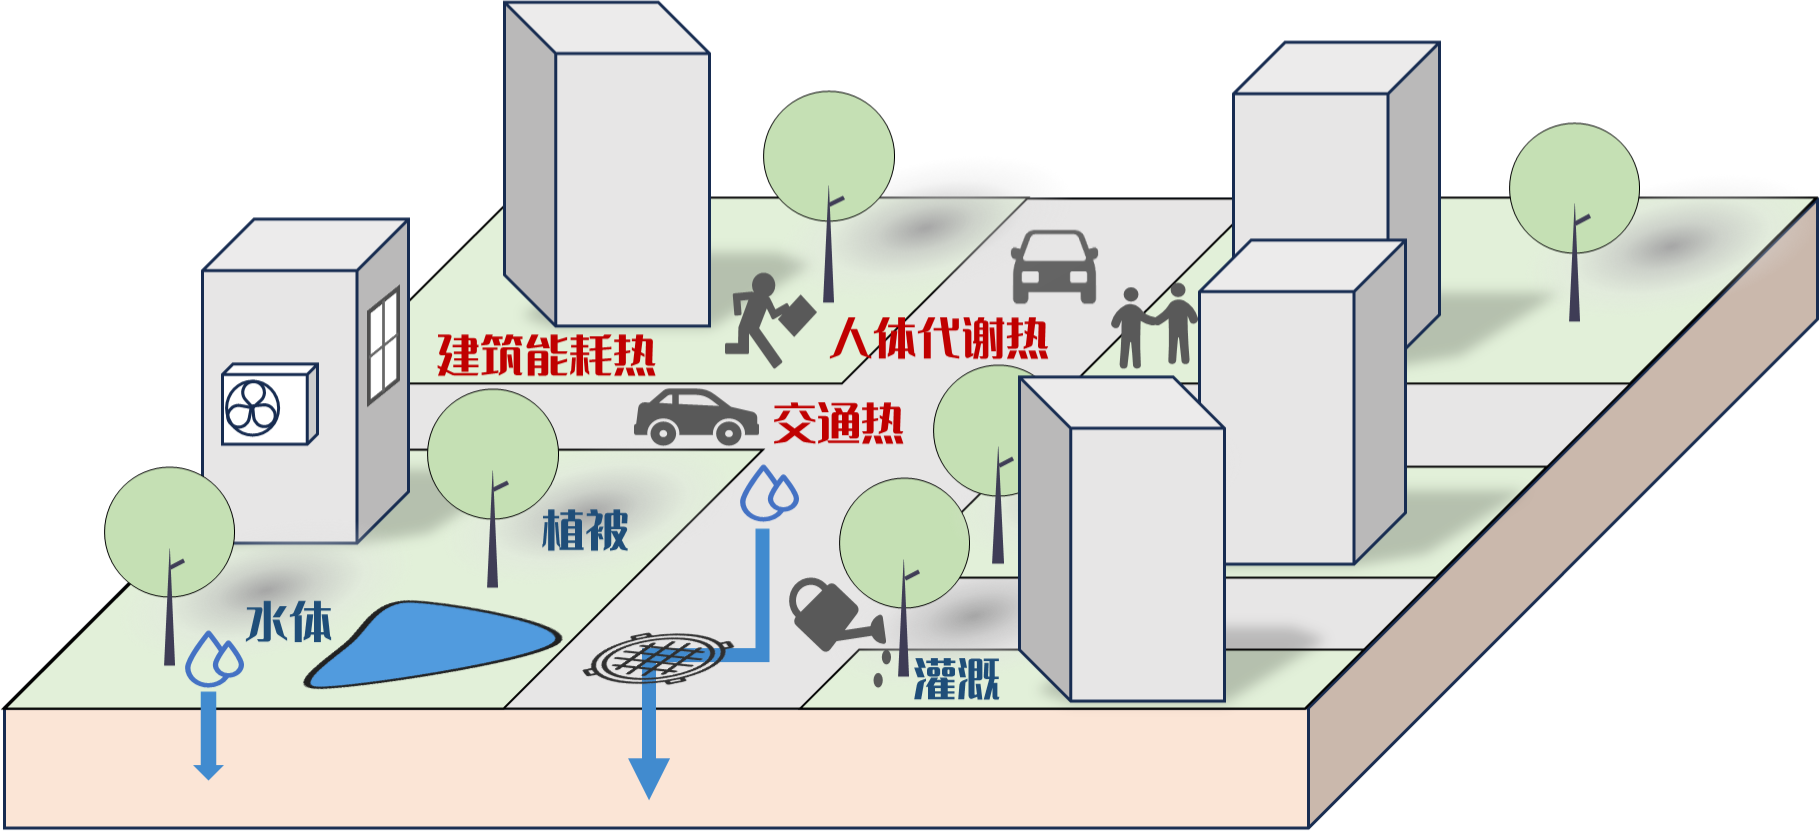
\includegraphics[width=0.9\textwidth]{Figures/城市模式/CoLM城市模式概念图.png}
    \caption{CoLM城市模式概念图}
    \label{fig:CoLM城市模式概念图}
  \end{figure}
}

\section{CoLM城市模式结构与功能}
\esection{CoLM Urban Model Structure and Functions}
不同于传统的城市街谷假设模型,CoLM采用由单栋建筑物组成的建筑群落来表征城市,如图~\ref{fig:CoLM城市模式结构和功能示意图} 所示。
建筑物随机分布,包括建筑物位置及朝向。城市几何参数包括建筑物覆盖度$f_{\rm b}$ (即屋顶覆盖面积占比$f_{\mathrm{roof}}$),地面(透水、不透水面)覆盖度$f_{\rm g}$ ($f_{\mathrm{gimp}}$,$f_{\mathrm{gper}}$),建筑物高度${\mathrm {H}}$,建筑物高度与建筑物平均边长比$\rm H/L$ (建筑物底面考虑为正方形,边长记为$\rm L$),植被冠层中心高度$h_{\rm v}$,城市树木叶面积指数 LAI 及茎面积指数 SAI,植被(树)覆盖面积比例记为$f_{\rm v}$。
其中$f_{\rm b}+f_{\rm g}=1$,$f_{\mathrm{gimp}}+f_{\mathrm{gper}}=1$。城市水体覆盖单独表征,其过程考虑为等效湖泊进行计算。

{
  \begin{figure}[htbp]
    \centering
    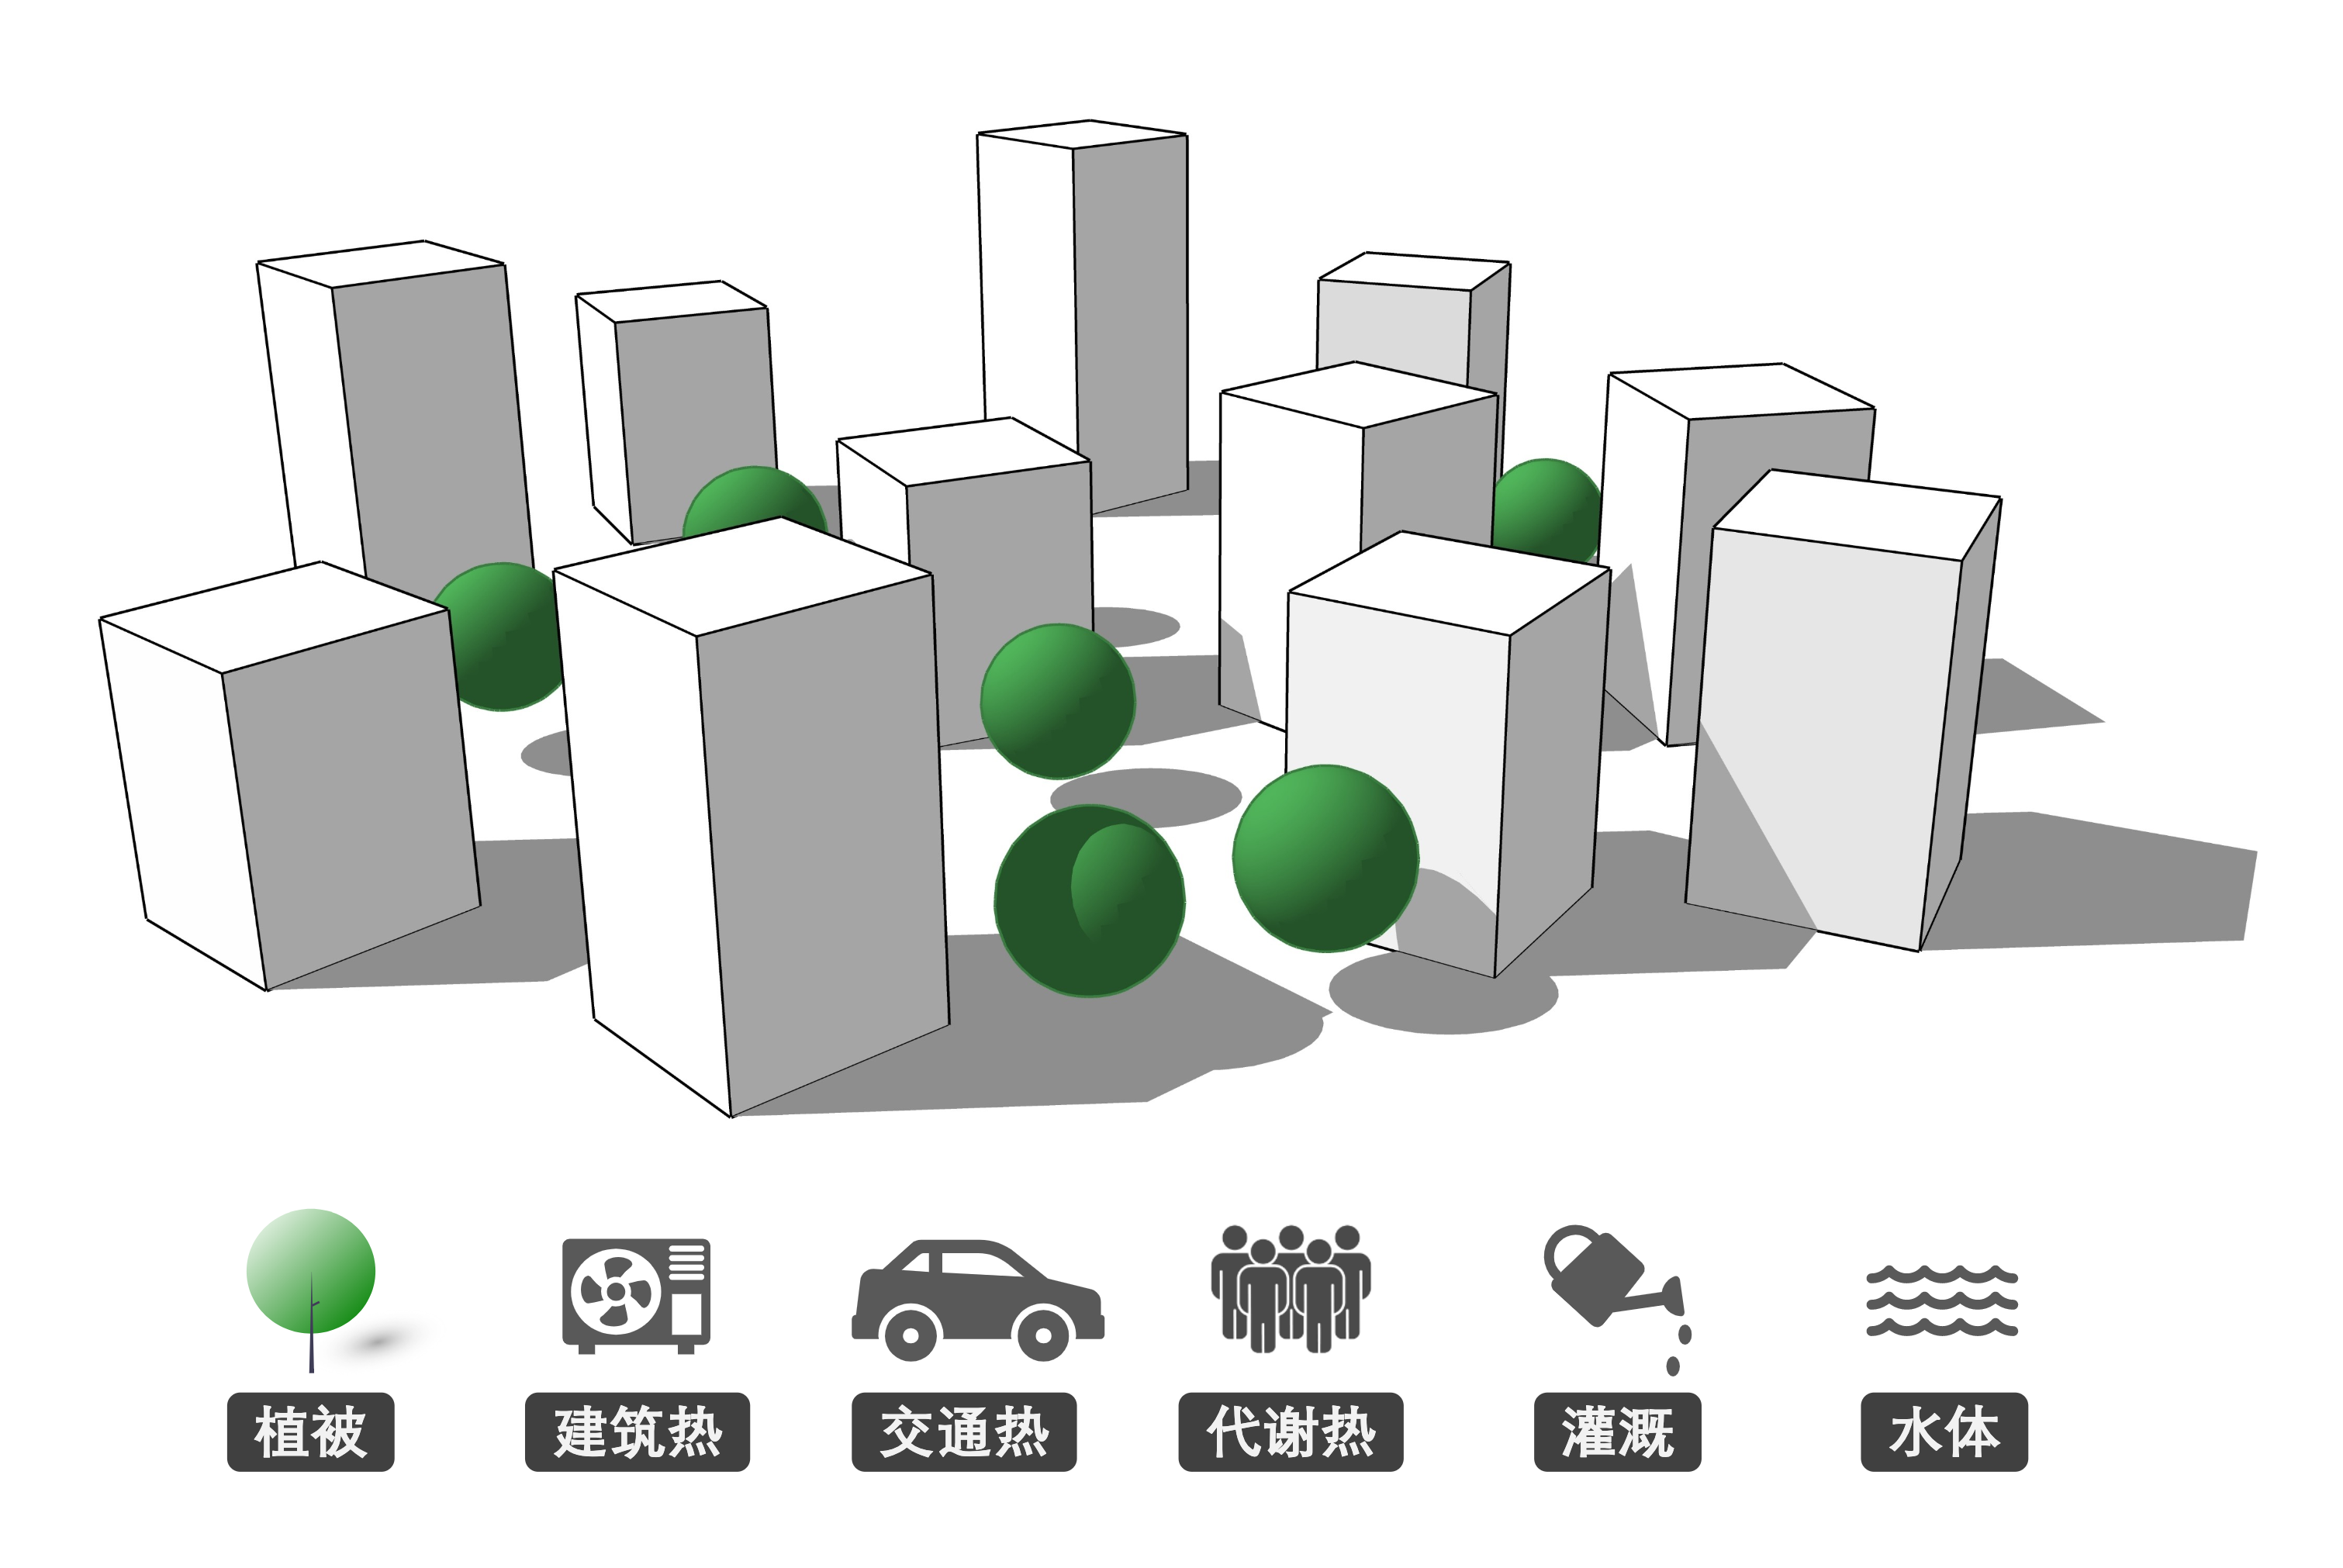
\includegraphics[width=0.8\textwidth]{Figures/城市模式/CoLM城市模式结构和功能示意图.png}
    \caption{CoLM城市模式结构和功能示意图}
    \label{fig:CoLM城市模式结构和功能示意图}
  \end{figure}
}

现有的城市模式往往不对平均单栋建筑物进行表征,而是采用街谷宽度比$\rm H/W$描述城市结构主要特征($\rm W$表示楼与楼之间平均距离)。在已知$f_{\rm b}$和$\rm H/W$参数,而未知$\rm L$时,$\rm L$可以简单计算为:
%
\begin{equation}
  \frac{\rm H}{\rm L}=\frac{\rm H}{\rm W} \cdot \frac{1-\sqrt{f_{\mathrm{b}}}}{\sqrt{f_{\mathrm{b}}}}, \text { 即 } {\rm L=W} \frac{\sqrt{f_{\mathrm{b}}}}{1-\sqrt{f_{\mathrm{b}}}}
\end{equation}
%
对于同一所在地城市覆盖,单栋建筑物几何参数一致,目前未显式考虑建筑物之间的几何差异,即以上参数代表统计平均值。

在以下分模块公式推导中,变量下标约定如下:天空($\rm {s}$),地面($\rm {g}$,包括透水面$\rm{gper}$和不透水面$\rm{gimp}$),墙面($\rm{w}$,包括阳面墙$\rm{wsun}$和阴面墙$\rm{wsha}$),植被($\rm{v}$)和屋顶$(\rm{roof}$)。$F$表示可视因子,例如$F_{\mathrm{gs}}$表示从地面到天空的可视因子。
$S$表示阴影面积占比,$\rm H/W$在推导过程中表示为$\rm HW$,$\rm H/L$表示为$\rm HL$,总的直射入射和漫射入射太阳辐射能量通量采用单位能量1表示。

{
  \begin{figure}[htbp]
    \centering
    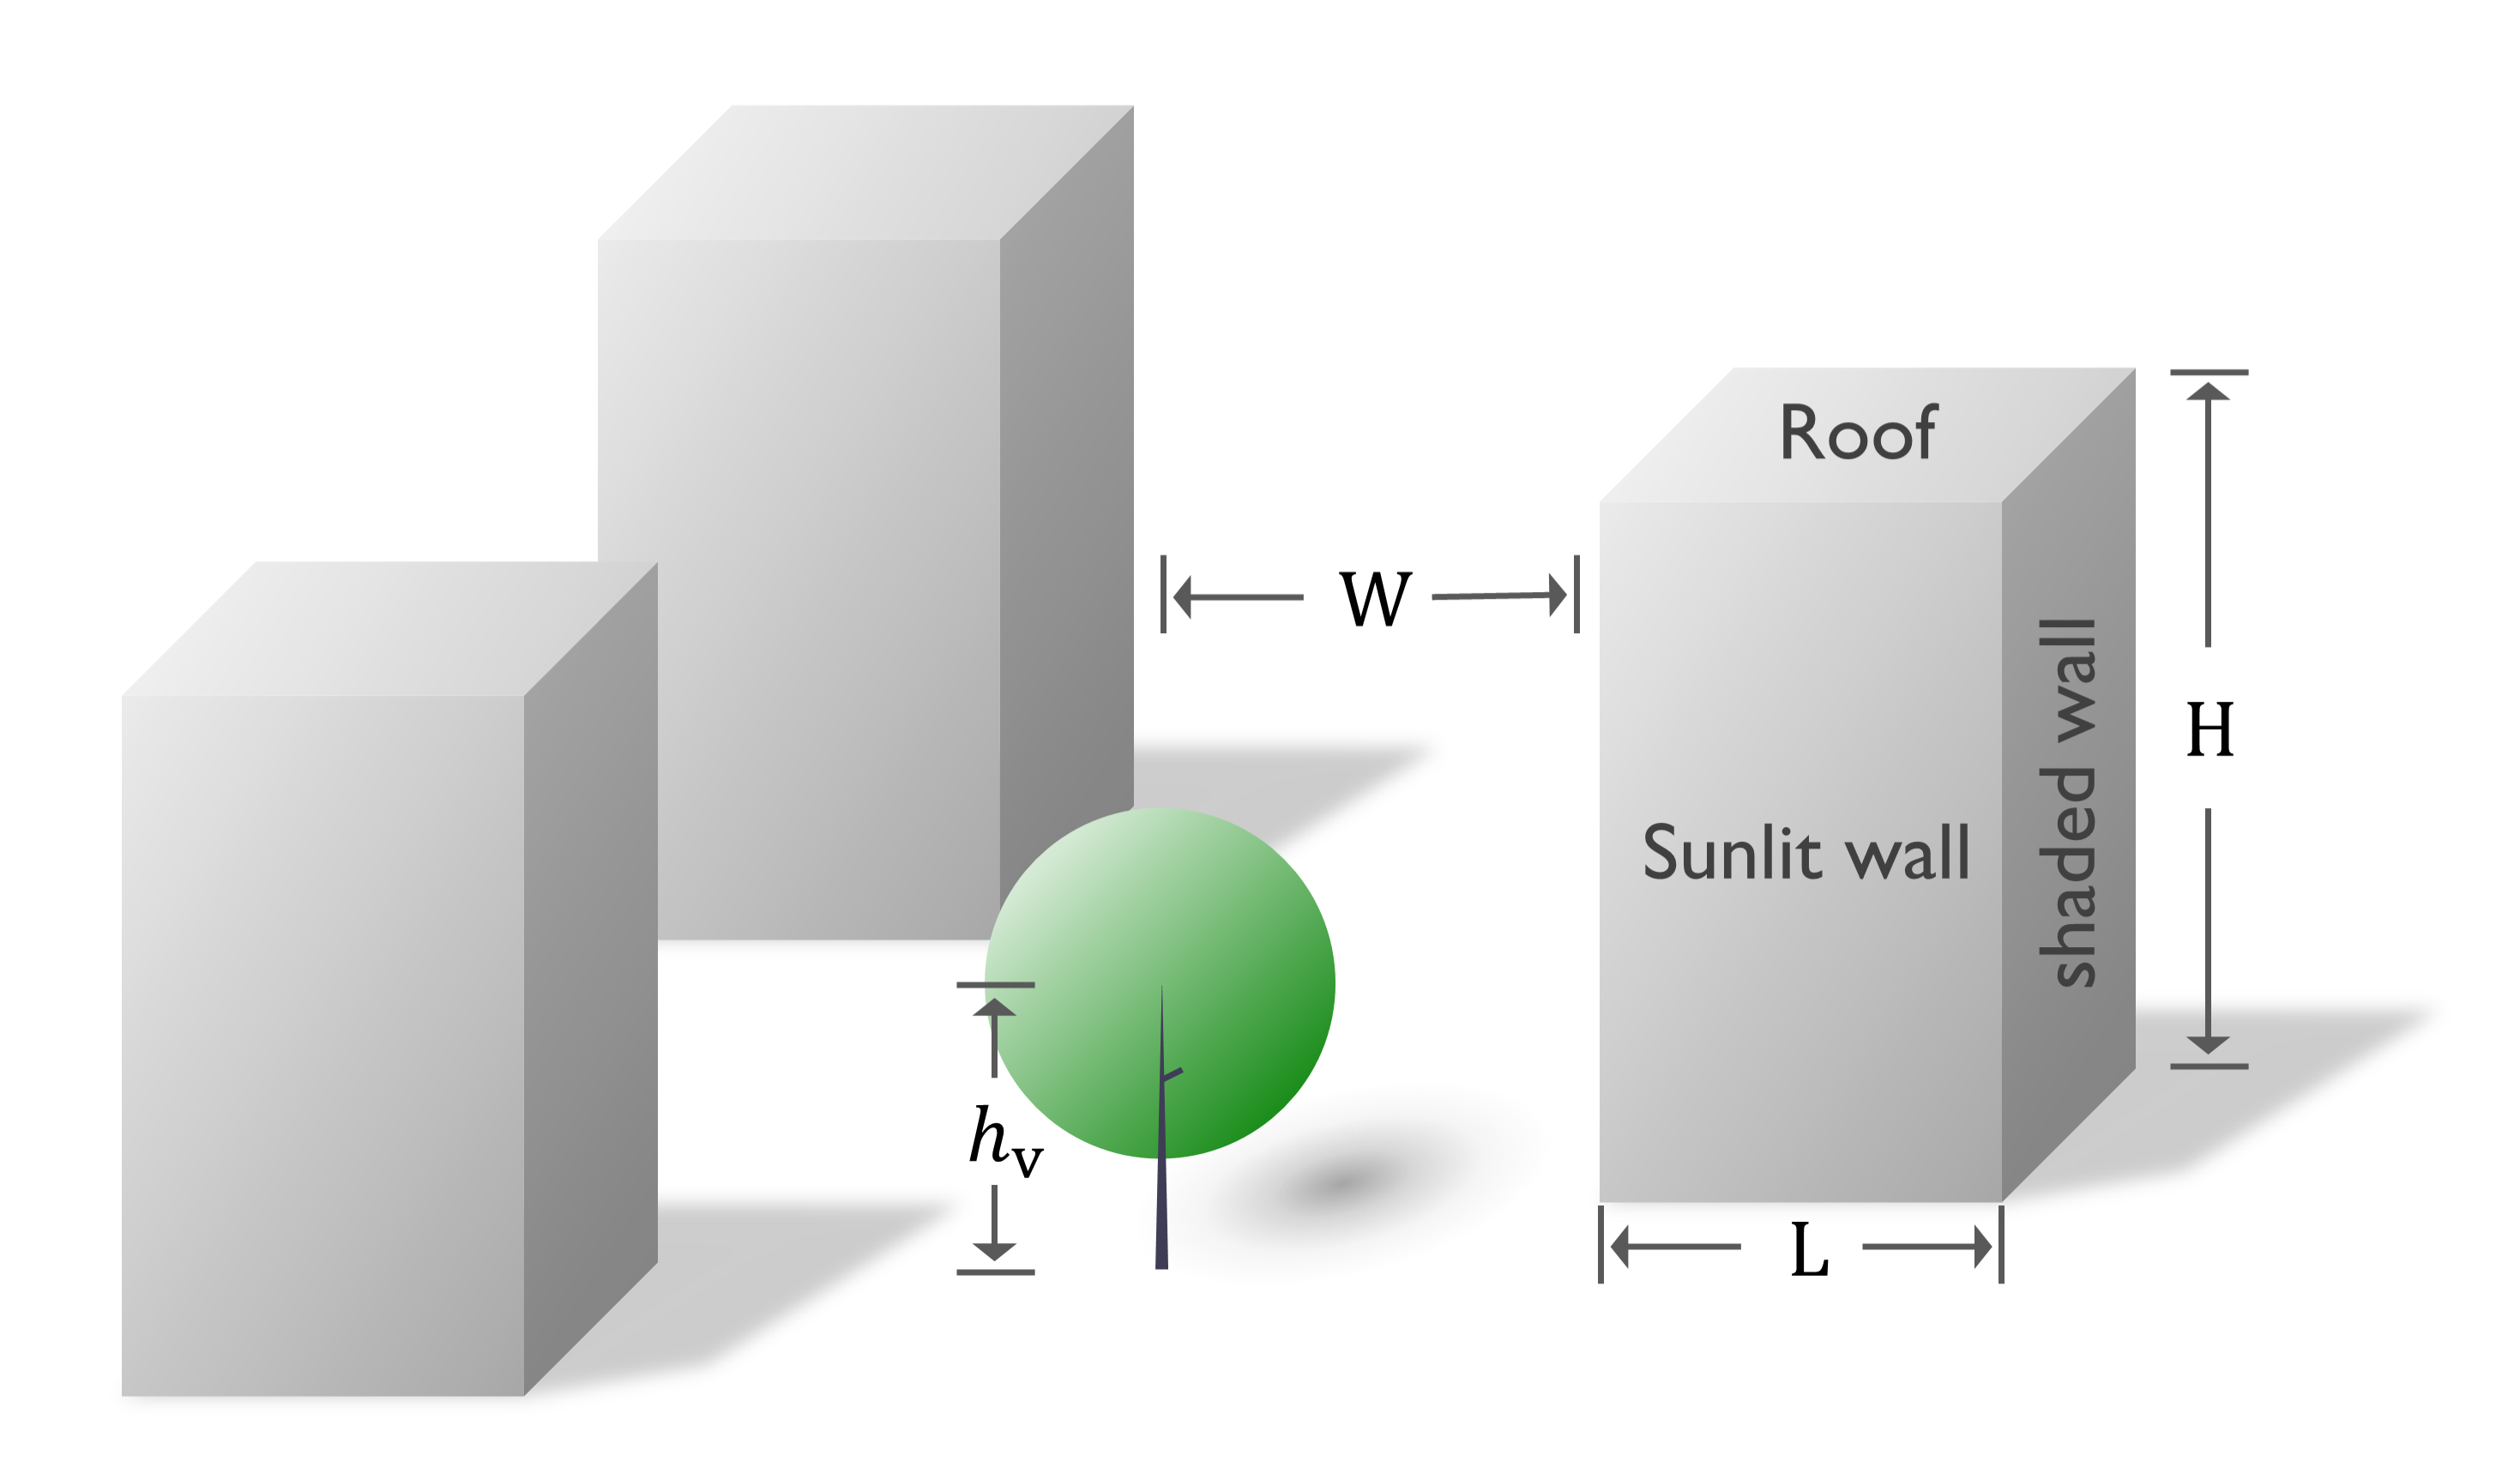
\includegraphics[width=0.7\textwidth]{Figures/城市模式/CoLM城市模式建筑植被结构示意图_v2.png}
    \caption{CoLM城市模式建筑及植被几何结构示意图}
    \label{fig:CoLM城市模式几何结构示意图}
  \end{figure}
}


\section{短波辐射传输}\label{短波辐射传输}
\esection{Shortwave Radiation Transfer}
\begin{mymdframed}{代码}
  本章节对应代码包含于\texttt{URBAN/MOD\_Urban\_Shortwave.F90}。
\end{mymdframed}

\subsection{无植被覆盖时短波辐射传输}\label{无植被覆盖时短波辐射传输}
\esubsection{Without Vegetation}
\begin{mymdframed}{代码}
  本部分对应代码为\texttt{URBAN/MOD\_Urban\_Shortwave.F90}文件中\texttt{UrbanOnlyShortwave}函数。
\end{mymdframed}

总体思路:计算考虑建筑物相互遮挡时的地面阴影面积、阳面墙和阴面墙面积;计算天空、墙面和地面之间的可视因子$F$;计算初始达到各组成面的辐射量,考虑之间多次散射过程,建立辐射传输平衡方程进行求解,具体过程如下。

太阳辐射直射照射时(太阳天顶角$\theta_{\rm s}$),
建筑物群落在地面的阴影覆盖占比(被墙面遮挡的部分)计算为:
\begin{equation}\label{S_w}
  S_{\mathrm{w}}=1-\exp \left(-\frac{4}{\pi} \cdot \frac{f_{\mathrm{b}}}{f_{\mathrm{g}}} {\rm HL} \cdot \tan \left(\theta_{\mathrm{s}}\right)\right)
\end{equation}
阳面墙面积相对总墙面占比计算为:
\begin{equation}\label{f_wsun}
  f_{\mathrm{wsun}}=0.5 \cdot \frac{S_{\mathrm{w}} f_{\mathrm{g}}+f_{\mathrm{b}}}{\frac{4}{\pi} f_{\mathrm{b}} {\rm HL} \tan \left(\theta_{\mathrm{s}}\right)+f_{\mathrm{b}}}
\end{equation}
阴面墙面积占比:
\begin{equation}\label{f_wsha}
  f_{\mathrm{wsha}}=1-f_{\mathrm{wsun}}
\end{equation}
墙面总面积可计算为$4{\rm HL}f_{\rm b}$。对于天空到墙面的可视因子$F_{\mathrm{sw}}$,即天空漫射光源到达墙面的辐射部分,其计算类似于直射光在被墙面遮挡的面积比例:
\begin{equation}\label{f_sw}
  F_{\mathrm{sw}}=1-\exp \left(-\frac{4}{\pi} \cdot \frac{f_{\mathrm{b}}}{f_{\mathrm{g}}} {\rm HL} \cdot \tan \left(\theta_{\mathrm{s}}^{*}\right)\right)
\end{equation}
其中$\theta_{\rm s}^\ast$为漫射光情况下等效角度,可近似计算为:
\begin{equation}
  \theta_{\mathrm{s}}^{*}=\frac{53-10 \sqrt{\frac{f_{\mathrm{b}}}{f_{\mathrm{g}}} {\rm HL}}}{180} \cdot \pi
\end{equation}
根据能量守恒,天空到达地面的可视因子$F_{\mathrm{sg}}=1-F_{\mathrm{sw}}$。
根据可视因子对称性,地面到达墙面和天空的可视因子$F_{\mathrm{gw}}=F_{\mathrm{sw}}$,$F_{\mathrm{gs}}=F_{\mathrm{sg}}$。
墙面到天空和地面的可视因子($F_{\mathrm{ws}}$, $F_{\mathrm{wg}}$)根据互易原理,满足如下关系:
\begin{equation}
  F_{\mathrm{ws}} \cdot 4 {\rm HL} f_{\mathrm{b}}=F_{\mathrm{s w}} \cdot f_{\mathrm{g}}
\end{equation}
\begin{equation}
  F_{\mathrm{wg}} \cdot 4 {\rm HL} f_{\mathrm{b}}=F_{\mathrm{s w}} \cdot f_{\mathrm{g}}
\end{equation}
由于太阳辐射在墙面垂直分布并不均匀,建筑物上半部分偏多,下半部分偏少,对上式进行简单调整,$F_{\mathrm{ws}}$和$F_{\mathrm{wg}}$计算为:
\begin{equation}
  F_{\mathrm{ws}}=0.75 F_{\mathrm{s w}} \frac{f_{\mathrm{g}}}{f_{\mathrm{b}}} \frac{1}{2 {\rm HL}}
\end{equation}
\begin{equation}
  F_{\mathrm{wg}}=0.25 F_{\mathrm{s w}} \frac{f_{\mathrm{g}}}{f_{\mathrm{b}}} \frac{1}{2 {\rm HL}}
\end{equation}
再根据能量守恒,墙面到墙面的可视因子$F_{\mathrm{ww}}$计算为:
\begin{equation}
  F_{\mathrm{ww}}=1-F_{\mathrm{ws}}-F_{\mathrm{wg}}
\end{equation}

\textit{1. 直射入射太阳辐射}

对于直射入射太阳辐射,直射光到达阳面墙的辐射通量$E_{\mathrm{wsun}}=S_{\rm w}$,即墙面在地面的阴影覆盖比例。
到达阴面墙的辐射通量$E_{\mathrm{wsha}}=0$,到达地面的辐射通量$E_{\rm g}=1-E_{\mathrm{wsun}}$,
其中$E_{\mathrm{gimp}}=E_{\rm g}f_{\mathrm{gimp}}$,$E_{\mathrm{gper}}=E_{\rm g}f_{\mathrm{gper}}$。
阳面墙、阴面墙、不透水面和透水面第一次散射辐射通量可分别计算为:
$E_{\mathrm{wsun}}\alpha_{\rm w}$,$E_{\mathrm{wsha}}\alpha_{\rm w}$,$E_{\mathrm{gimp}}\alpha_{\mathrm{gimp}}$,$E_{\mathrm{gper}}\alpha_{\mathrm{gper}}$。
其中$\alpha$表示反照率,不分区阳面和阴面。所有组成面均不区分漫射和直射照射反照率,且反射后的辐射假设为漫射辐射。
当经过墙面地面之间多次散射后,达到辐射平衡时的墙面和地面辐射出射通量记为$M$,可建立如下辐射平衡方程:
\begin{landscape}
  \begin{equation}
    \begin{aligned}
      M_{\mathrm{ {wsun }}} &=E_{\mathrm{wsun}} \alpha_{\mathrm{w}}+M_{\mathrm{wsun}} F_{\mathrm{ww}} f_{\mathrm{wsun}} \alpha_{\mathrm{w}}+M_{\mathrm{wsha}} F_{\mathrm{ww}} f_{\mathrm{wsun}} \alpha_{\mathrm{w}}+M_{\mathrm{gimp}} F_{\mathrm{g w}} f_{\mathrm{wsun}} \alpha_{\mathrm{w}}+M_{\mathrm{gper}} F_{\mathrm{g w}} f_{\mathrm{wsun}} \alpha_{\mathrm{w}} \\
      M_{\mathrm{wsha}} &=E_{\mathrm{wsha}} \alpha_{\mathrm{w}}+M_{\mathrm{wsha}} F_{\mathrm{ww}} f_{\mathrm{wsha}} \alpha_{\mathrm{w}}+M_{\mathrm{wsun}} F_{\mathrm{ww}} f_{\mathrm{wsha}} \alpha_{\mathrm{w}}+M_{\mathrm{gimp}} F_{\mathrm{g w}} f_{\mathrm{wsha}} \alpha_{\mathrm{w}}+M_{\mathrm{gper}} F_{\mathrm{g w}} f_{\mathrm{wsha}} \alpha_{\mathrm{w}} \\
      M_{\mathrm{gimp}} &=E_{\mathrm{gimp}} \alpha_{\mathrm{gimp}}+M_{\mathrm{wsun}} F_{\mathrm{w g}} f_{\mathrm{ gimp}} \alpha_{\mathrm{gimp}}+M_{\mathrm{wsha}} F_{\mathrm{w g}} f_{\mathrm{ gimp}} \alpha_{\mathrm{gimp}} \\
      M_{\mathrm{gper}} &=E_{\mathrm{gper}} \alpha_{\mathrm{gper}}+M_{\mathrm{wsun}} F_{\mathrm{w g}} f_{\mathrm{gper}} \alpha_{\mathrm{gper}}+M_{\mathrm{wsha}} F_{\mathrm{w g}} f_{\mathrm{gper}} \alpha_{\mathrm{gper}}
    \end{aligned}
  \end{equation}
  通过整理得到:
  \begin{equation}\label{城市无植被辐射传输方程}
    \left(\begin{array}{cccc}1-F_{\mathrm{ww}} f_{\mathrm{wsun}} \alpha_{\mathrm{w}} & -F_{\mathrm{ww}} f_{\mathrm{wsun}} \alpha_{\mathrm{w}} & -F_{\mathrm{g w}} f_{\mathrm{wsun}} \alpha_{\mathrm{w}} & -F_{\mathrm{g w}} f_{\mathrm{wsun}} \alpha_{\mathrm{w}} \\
        -F_{\mathrm{ww}} f_{\mathrm{wsha}} \alpha_{\mathrm{w}} & 1-F_{\mathrm{ww}} f_{\mathrm{wsha}} \alpha_{\mathrm{w}} & -F_{\mathrm{g w}} f_{\mathrm{wsha}} \alpha_{\mathrm{w}} & -F_{\mathrm{g w}} f_{\mathrm{wsha}} \alpha_{\mathrm{w}} \\
        -F_{\mathrm{w g}} f_{\mathrm{gimp}} \alpha_{\mathrm{gimp}} & -F_{\mathrm{w g}} f_{\mathrm{gimp}} \alpha_{\mathrm{gimp}} & 1 & 0 \\
    -F_{\mathrm{w g}} f_{\mathrm{gper}} \alpha_{\mathrm{gper}} & -F_{\mathrm{w g}} f_{\mathrm{gper}} \alpha_{\mathrm{gper}} & 0 & 1\end{array}\right)
    \left(\begin{array}{l}M_{\mathrm{wsun}} \\ M_{\mathrm{ {wsha }}} \\
        M_{\mathrm{ gimp}} \\
    M_{\mathrm{gper}}\end{array}\right)=\left(\begin{array}{c}E_{\mathrm{wsun}} \alpha_{\mathrm{w}} \\
        E_{\mathrm{wsha}} \alpha_{\mathrm{w}} \\
        E_{\mathrm{gimp}} \alpha_{\mathrm{ gimp}} \\
    E_{\mathrm{gper}} \alpha_{\mathrm{gper}}\end{array}\right)
  \end{equation}
\end{landscape}

经过整理的公式(\ref{城市无植被辐射传输方程})可简单表示为
\begin{equation}\label{mathbf_AX}
  \mathbf{A x}=\mathbf{B}
\end{equation}
$\mathbf{A}$为辐射传输矩阵,$\mathbf{B}$为向量($E_{\mathrm{wsun}}\alpha_{\rm w}$, $E_{\mathrm{wsha}}\alpha_{\rm w}$, $E_{\mathrm{gimp}}\alpha_{\mathrm{gimp}}$, $E_{\mathrm{gper}}\alpha_{\mathrm{gper}}$),
即太阳辐射到达墙面和地面后第一次反射的辐射通量。$\mathbf{x}$为求解变量组成的向量(\allowbreak$M_{\mathrm{wsun}}$, \allowbreak$M_{\mathrm{wsha}}$, \allowbreak$M_{\mathrm{gimp}}$, \allowbreak$M_{\mathrm{gper}}$),
计算为:
\begin{equation}\label{mathbf_X}
  \mathbf{x}=\mathbf{A}^{-1} \mathbf{B}
\end{equation}
矩阵$\mathbf{A}$是由已知变量组成的常数矩阵,可直接进行求逆计算,向量$\mathbf{B}$已给出,因此可计算得到$\mathbf{x}$。从而墙面和地面的辐射吸收计算为:
\begin{equation}\label{s_wsun_wsha_gimp_gper_1}
  \begin{aligned}s_{\mathrm{wsun}} &=\frac{M_{\mathrm{wsun}}}{\alpha_{\mathrm{w}}}\left(1-\alpha_{\mathrm{w}}\right) \\
    s_{\mathrm{wsha}} &=\frac{M_{\mathrm{wsha}}}{\alpha_{\mathrm{w}}}\left(1-\alpha_{\mathrm{w}}\right) \\
    s_{\mathrm{gimp}} &=\frac{M_{\mathrm{gimp}}}{\alpha_{\mathrm{gimp}}}\left(1-\alpha_{\mathrm{gimp}}\right) \\
  s_{\mathrm{gper}} &=\frac{M_{\mathrm{gper}}}{\alpha_{\mathrm{gper}}}\left(1-\alpha_{\mathrm{gper}}\right)\end{aligned}
\end{equation}
注意,以上辐射吸收为各组成面总吸收量,其各自单位面积辐射吸收量修改为:
\begin{equation}\label{s_wsun_wsha_gimp_gper_2}
  \begin{aligned}s_{\mathrm{wsun}} &=\frac{f_{\mathrm{g}}}{4 f_{\mathrm{wsun}} \mathrm{HL} f_{\mathrm{b}}} s_{\mathrm{wsun}} \\
    s_{\mathrm{wsha}} &=\frac{f_{\mathrm{g}}}{4 f_{\mathrm{wsha}} \mathrm{HL} f_{\mathrm{b}}} s_{\mathrm{wsha}} \\
    s_{\mathrm{gimp}} &=\frac{1}{f_{\mathrm{gimp}}} s_{\mathrm{gimp}} \\
  s_{\mathrm{gper}} &=\frac{1}{f_{\mathrm{gper}}} s_{\mathrm{gper}}\end{aligned}
\end{equation}
不考虑屋顶时的城市反照率为:
\begin{equation}\label{alpha_u}
  \alpha_{\mathrm{u}}=M_{\mathrm{wsun}} F_{\mathrm{ws}}+M_{\mathrm{wsha}} F_{\mathrm{ws}}+M_{\mathrm{gimp}} F_{\mathrm{gs}}+M_{\mathrm{gper}} F_{\mathrm{gs}}
\end{equation}
屋顶的吸收计算为$s_{\mathrm{roof}}=1-\alpha_{\mathrm{roof}}$,考虑屋顶的城市反照率(\ref{alpha_u})修订为:
\begin{equation}\label{alpha_u2}
  \alpha_{\mathrm{u}}=\alpha_{\mathrm{{roof }}} f_{\mathrm{roof}}+\alpha_{\mathrm{u}} f_{\mathrm{g}}
\end{equation}

对于城市水体(湖泊)考虑方式同屋顶,最终城市区域地表反照率为各自面积加权平均,计算方式类似于公式~\eqref{alpha_u2}。

\textit{2. 漫射入射太阳辐射}

对于漫射情况,计算过程与直射入射辐射基本类似,同样采用公式(\ref{城市无植被辐射传输方程})所示的矩阵形式进行求解,不同之处在于初始到达墙面和地面后第一次反射的辐射通量,分别计算为:
$F_{\mathrm{sw}}f_{\mathrm{wsun}}\alpha_{\rm w}$,$F_{\mathrm{sw}}f_{\mathrm{wsha}}\alpha_{\rm w}$,$F_{\mathrm{sg}}f_{\mathrm{gimp}}\alpha_{\rm gimp}$,$F_{\mathrm{sg}}f_{\mathrm{gper}}\alpha_{\rm gper}$,即公式(\ref{mathbf_AX})中的$\mathbf{B}$。
漫射入射辐射的传输矩阵同直射入射辐射情景,即$\mathbf{A}$。其求逆后的结果可以直接用于漫射入射辐射,利用公式(\ref{mathbf_X})计算得到墙面和地面的辐射出射通量。
单位面积的辐射吸收和城市反照率计算同公式(\ref{s_wsun_wsha_gimp_gper_2})、(\ref{alpha_u})和(\ref{alpha_u2}),在此不再列出。

\subsection{有植被覆盖时短波辐射传输}\label{有植被覆盖时短波辐射传输}
\esubsection{With Vegetation}
\begin{mymdframed}{代码}
  本部分对应代码为\texttt{URBAN/MOD\_Urban\_Shortwave.F90}文件中\texttt{UrbanVegShortwave}函数。
\end{mymdframed}

城市中考虑植被后的短波辐射传输过程是在无植被辐射传输的基础上,考虑植被在内的各组成面之间的可视因子,从而构建辐射传输平衡方程,采用类似的方法求解墙面、地面和植被的辐射吸收。
相比章节~\ref{无植被覆盖时短波辐射传输} 增加的部分为考虑植被在内的可视因子和阴影面积计算。

在植被树冠中心高度$h_{\rm v}$处,墙面的阴影比例可根据公式(\ref{S_w})计算,利用$\frac{{\rm H}-h_{\rm v}}{\rm L}$代替$\rm HL$,记为$S_{\rm w}^\prime$,即
\begin{equation}
  S_{\mathrm{w}}^{\prime}=1-\exp \left(-\frac{4}{\pi} \cdot \frac{f_{\mathrm{b}}}{f_{\mathrm{g}}} \frac{{\rm H}-h_{\mathrm{v}}}{\rm L} \cdot \tan \left(\theta_{\mathrm{s}}\right)\right)
\end{equation}
假设该阴影部分与植被覆盖$f_{\rm v}$随机重叠,则植被被阴影遮挡的面积比例为$f_{\rm v}S_{\mathrm {w}} ^\prime$,未被遮挡的植被覆盖面积占比为$f_{\rm v}^\prime=f_{\rm v}-f_{\rm v}S_{\rm w}^\prime$。
未被遮挡植被在整个城市覆盖区域的阴影覆盖$S_{\rm v}$可根据公式(\ref{S_area})计算得到。将其阴影覆盖比例转化为地面所占比例为:
\begin{equation}\label{S_v2}
  S_{\mathrm{v}}=S_{\mathrm{v}} / f_{\mathrm{g}}
\end{equation}

假设墙面在地面的阴影占比与植被的阴影随机重叠,则重叠部分$S_{\mathrm{vw}}$计算为:
\begin{equation}
  S_{\mathrm{v w}}=S_{\mathrm{v}}\left(S_{\mathrm{w}}-S_{\mathrm{w}}^{\prime}\right)
\end{equation}
该重叠部分假设全部为植被遮挡墙面。在地面覆盖区域,墙面的阴影占比修正为:
\begin{equation}\label{S_w2}
  S_{\mathrm{w}}=S_{\mathrm{w}}-S_{\mathrm{v w}}
\end{equation}
阴面墙和阳面墙的面积占比计算同公式(\ref{f_wsun})和(\ref{f_wsha})。

在不考虑植被存在时,可视因子$F_{\mathrm{sw}}$, $F_{\mathrm{sg}}$, $F_{\mathrm{gw}}$, $F_{\mathrm{gs}}$, $F_{\mathrm{ws}}$, $F_{\mathrm{wg}}$ 和 $F_{\mathrm{ww}}$的
计算同章节~\ref{无植被覆盖时短波辐射传输}。下面需要考虑植被的遮挡,对以上可视因子进行修改,并添加植被到各个面的可视因子。

同公式(\ref{S_v2})和(\ref{S_w2}),计算在漫射等效角度下的墙面和植被在地面的“阴影”占比(辐射遮挡) $S_{\rm w}^\ast$和$S_{\rm v}^\ast$,
利用公式(\ref{f_sw})进行计算,则天空到达植被($F_{\mathrm{sv}}$)、天空通过植被到墙面($F_{\mathrm{svw}}$),以及天空通过植被到达地面的可视因子($F_{\mathrm{svg}}$)分别计算为:
\begin{equation}\label{F_sv_svw_svg}
  \begin{aligned}F_{\mathrm{s v}} &=S_{\mathrm{v}}^{*} \\ F_{\mathrm{s v w}} &=S_{\mathrm{v w}}^{*} \\ F_{\mathrm{s v g}} &=F_{\mathrm{s v}}-F_{\mathrm{s v w}}\end{aligned}
\end{equation}
假设植被到达天空的可视因子($F_{\mathrm{vs}}$)满足互易原理:
\begin{equation}
  F_{\mathrm{vs}}\cdot 2f_{\rm g} = \left( 1-S_{\rm w} ^{*\prime} \right ) \cdot f_{\rm g}
\end{equation}
其中$S_{\rm w} ^{*\prime}$为漫射辐射时,建筑在植被中心高度$h_{\rm v}$的“阴影”占比。可以得到:
\begin{equation}\label{eq:f_vs}
  F_{\mathrm{vs}} = 0.5 \left( 1-S_{\rm w} ^{*\prime} \right )
\end{equation}
同理,地面到达植被($F_{\mathrm{gv}}$)、地面通过植被到天空($F_{\mathrm{gvs}}$),以及地面通过植被到达天空的可视因子($F_{\mathrm{gvs}}$)可类似公式(\ref{F_sv_svw_svg})计算,植被到达地面的可视因子($F_{\mathrm{vg}}$)可类似公式(\ref{eq:f_vs})计算。再根据能量守恒,植被到达墙面的可视因子($F_{\mathrm{vw}}$)计算为:
%根据可视因子计算互易性原理,植被到天空、地面和墙面的可视因子计算为:
%\begin{equation}
%F_{\mathrm{vs}}=F_{\mathrm{sv}} \frac{f_{\rm g}}{4 f_{\rm v}}
%\end{equation}
%\begin{equation}
%F_{\mathrm{vg}}=F_{\mathrm{gv}} \frac{f_{\rm g}}{4 f_{\rm v}}
%\end{equation}
\begin{equation}
  F_{\mathrm{v w}}=1-F_{\mathrm{v s}}-F_{\mathrm{v g}}
\end{equation}
假设$F_{\mathrm{wv}}$满足如下互异性表达式:
\begin{equation}
  F_{\mathrm{vw}}\cdot 2f_{\rm g} \cdot 0.5\left( F_{\mathrm{sv}}+F_{\mathrm{gv}} \right ) = F_{\mathrm{wv}} \cdot 4 {\rm HL} f_{\rm b}
\end{equation}
从而得到:
\begin{equation}
  F_{\mathrm{wv}}=\frac{f_{\rm g} \cdot \left( F_{\mathrm{sv}}+F_{\mathrm{gv}} \right )} {4 {\rm HL}f_{\rm b}} F_{\mathrm{vw}}
\end{equation}
将上式$F_{\mathrm{wv}}$计算的结果限制为:
\begin{equation}
  F_{\mathrm{wv}} = \min \big(0.8, \max (f_{\rm v}, F_{\mathrm{wv}})\big)
\end{equation}
假设墙面通过植被到达墙面、天空和地面的可视因子与墙面到达相应各面的可视因子成正比,即:
\begin{equation}
  F_{\mathrm{wvw}}: F_{\mathrm{wvs}}: F_{\mathrm{wvg}}=F_{\mathrm{ww}}: f_{\mathrm{1}} F_{\mathrm{ws}}: f_{\mathrm{2}} F_{\mathrm{w g}}
\end{equation}
其中$f_1=h_{\rm v}/{\rm H}$,$f_2=\left({\rm H}-h_{\rm v}\right)/{\rm H}$。根据能量守恒:
\begin{equation}
  F_{\mathrm{wvw}}+F_{\mathrm{wvs}}+F_{\mathrm{wvg}}=F_{\mathrm{w v}}
\end{equation}
以上两式联立求解可得到:
\begin{equation}
  F_{\mathrm{wvw}}=\frac{F_{\mathrm{w v}} F_{\mathrm{ww}}}{F_{\mathrm{ww}}+f_{\mathrm{1}} F_{\mathrm{ws}}+f_{\mathrm{2}} F_{\mathrm{w g}}}
\end{equation}
\begin{equation}
  F_{\mathrm{wvs}}=f_{\mathrm{1}} \frac{F_{\mathrm{ws}}}{F_{\mathrm{ww}}} F_{\mathrm{wvw}}
\end{equation}
\begin{equation}
  F_{\mathrm{wvg}}=f_{\mathrm{2}} \frac{F_{\mathrm{w g}}}{F_{\mathrm{ww}}} F_{\mathrm{wvw}}
\end{equation}
在此基础上,可以计算得到考虑植被影响的天空、墙面和地面之间的可视因子,
其中天空到墙面和地面的可视因子$F_{\mathrm{sw}}^\prime$, $F_{\mathrm{sg}}^\prime$计算为:
\begin{equation}
  F_{\mathrm{sw}}^{\prime}=F_{\mathrm{sw}}-F_{\mathrm{svw}}+F_{\mathrm{svw}} T_{\mathrm{d}}
\end{equation}
\begin{equation}
  F_{\mathrm{sg}}^{\prime}=F_{\mathrm{sg}}-F_{\mathrm{svg}}+F_{\mathrm{svg}} T_{\mathrm{d}}
\end{equation}
其中$T_{\mathrm {d}}$为单棵球形树冠直射透射率,利用公式(\ref{T_ds_tau})计算。
地面到达墙面和天空的可视因子$F_{\mathrm{gw}}^\prime$, $F_{\mathrm{gs}}^\prime$计算为:
\begin{equation}
  F_{\mathrm{gw}}^{\prime}=F_{\mathrm{gw}}-F_{\mathrm{gvw}}+F_{\mathrm{gvw}} T_{\mathrm{d}}
\end{equation}
\begin{equation}
  F_{\mathrm{gs}}^{\prime}=F_{\mathrm{gs}}-F_{\mathrm{gvs}}+F_{\mathrm{gvs}} T_{\mathrm{d}}
\end{equation}
墙面到达地面、墙面和天空的可视因子$F_{\mathrm{wg}}^\prime$, $F_{\mathrm{ww}}^\prime$, $F_{\mathrm{ws}}^\prime$计算为:
\begin{equation}
  F_{\mathrm{wg}}^{\prime}=F_{\mathrm{wg}}-F_{\mathrm{wvg}}+F_{\mathrm{wvg}} T_{\mathrm{d}}
\end{equation}
\begin{equation}
  F_{\mathrm{ww}}^{\prime}=F_{\mathrm{ww}}-F_{\mathrm{wvw}}+F_{\mathrm{wvw}} T_{\mathrm{d}}
\end{equation}
\begin{equation}
  F_{\mathrm{ws}}^{\prime}=F_{\mathrm{ww}}-F_{\mathrm{wvs}}+F_{\mathrm{wvs}} T_{\mathrm{d}}
\end{equation}

\textit{1. 直射入射太阳辐射}

对于直射入射太阳辐射,直射光到达阳面墙的辐射通量$E_{\mathrm{wsun}}=S_{\rm w}$,到达阴面墙的辐射通量$E_{\mathrm{wsha}}=S_{\mathrm{vw}}T_{\mathrm {d}}$,
到达地面的辐射通量$E_{\rm g}=1-S_{\rm w}-S_{\rm v}+\left(S_{\rm v}-S_{\mathrm{vw}}\right)T_{\mathrm {d}}$,其中$E_{\mathrm{gimp}}=E_{\rm g}f_{\mathrm{gimp}}$,$E_{\mathrm{gper}}=E_{\rm g}f_{\mathrm{gper}}$,
$E_{\rm v}=S_{\rm v}$。阳面墙、阴面墙、不透水面、透水面和植被第一次散射辐射通量可分别计算为:$E_{\mathrm{wsun}}\alpha_{\rm w}$,$E_{\mathrm{wsha}}\alpha_{\rm w}$,
$E_{\mathrm{gimp}}\alpha_{\mathrm{gimp}}$,$E_{\mathrm{gper}}\alpha_{\mathrm{gper}}$,$E_{\rm v}\alpha_{\rm v}$,
其中$\alpha$表示反照率(对于植被表示所有向外散射辐射与入射辐射比例),不分区阳面和阴面墙,不区分漫射和直射照射,且反射后的辐射假设为漫射辐射。经过墙面、地面和植被之间多次散射,达到辐射平衡时的墙面、地面和植被辐射出射通量用符号$M$表示,利用各组成面之间的可视因子,可建立如下辐射平衡方程:
\begin{landscape}
  \begin{equation}
    \begin{aligned}M_{\mathrm{wsun}} &=E_{\mathrm{wsun}} \alpha_{\mathrm{w}}+M_{\mathrm{wsun}} F_{\mathrm{ww}}^{\prime} f_{\mathrm{wsun}} \alpha_{\mathrm{w}}+M_{\mathrm{wsha}} F_{\mathrm{ww}}^{\prime} f_{\mathrm{wsun}} \alpha_{\mathrm{w}}+M_{\mathrm{gimp}} F_{\mathrm{g w}}^{\prime} f_{\mathrm{wsun}} \alpha_{\mathrm{w}}+M_{\mathrm{gper}} F_{\mathrm{g w}}^{\prime} f_{\mathrm{wsun}} \alpha_{\mathrm{w}}+M_{\mathrm{v}} F_{\mathrm{v w}} f_{\mathrm{wsun}} \alpha_{\mathrm{w}} \\ M_{\mathrm{wsha}} &=E_{\mathrm{wsha}} \alpha_{\mathrm{w}}+M_{\mathrm{wsha}} F_{\mathrm{ww}}^{\prime} f_{\mathrm{wsha}} \alpha_{\mathrm{w}}+M_{\mathrm{wsun}} F_{\mathrm{ww}}^{\prime} f_{\mathrm{wsha}} \alpha_{\mathrm{w}}+M_{\mathrm{gimp}} F_{\mathrm{g w}}^{\prime} f_{\mathrm{wsha}} \alpha_{\mathrm{w}}+M_{\mathrm{gper}} F_{\mathrm{g w}}^{\prime} f_{\mathrm{wsha}} \alpha_{\mathrm{w}}+M_{\mathrm{v}} F_{\mathrm{v w}} f_{\mathrm{wsha}} \alpha_{\mathrm{w}} \\ M_{\mathrm{gimp}} &=E_{\mathrm{gimp}} \alpha_{\mathrm{gimp}}+M_{\mathrm{wsun}} F_{\mathrm{w g}}^{\prime} f_{\mathrm{gimp}} \alpha_{\mathrm{gimp}}+M_{\mathrm{wsha}} F_{\mathrm{w g}}^{\prime} f_{\mathrm{gimp}} \alpha_{\mathrm{gimp}}+M_{\mathrm{v}} F_{\mathrm{v g}} f_{\mathrm{gimp}} \alpha_{\mathrm{gimp}} \\ M_{\mathrm{gper}} &=E_{\mathrm{gper}} \alpha_{\mathrm{gper}}+M_{\mathrm{wsun}} F_{\mathrm{w g}}^{\prime} f_{\mathrm{gper}} \alpha_{\mathrm{gper}}+M_{\mathrm{wsha}} F_{\mathrm{w g}}^{\prime} f_{\mathrm{gper}} \alpha_{\mathrm{gper}}+M_{\mathrm{v}} F_{\mathrm{v g}} f_{\mathrm{gper}} \alpha_{\mathrm{gper}} \\ M_{\mathrm{v}} &=E_{\mathrm{v}} \alpha_{\mathrm{v}}+M_{\mathrm{wsun}} F_{\mathrm{w v}} \alpha_{\mathrm{v}}+M_{\mathrm{wsha}} F_{\mathrm{w v}} \alpha_{\mathrm{v}}+M_{\mathrm{gimp}} F_{\mathrm{g v}} \alpha_{\mathrm{v}}+M_{\mathrm{gper}} F_{\mathrm{g v}} \alpha_{\mathrm{v}}\end{aligned}
  \end{equation}
  整理后化简为:
  \begin{equation}
    \left(\begin{array}{ccccc}1-F_{\mathrm{ww}}^{\prime} f_{\mathrm{wsun}} \alpha_{\mathrm{w}} & -F_{\mathrm{ww}}^{\prime} f_{\mathrm{wsun}} \alpha_{\mathrm{w}} & -F_{\mathrm{g w}}^{\prime} f_{\mathrm{wsun}} \alpha_{\mathrm{w}} & -F_{\mathrm{g w}}^{\prime} f_{\mathrm{wsun}} \alpha_{\mathrm{w}} & -F_{\mathrm{v w}} f_{\mathrm{wsun}} \alpha_{\mathrm{w}} \\ -F_{\mathrm{ww}}^{\prime} f_{\mathrm{wsha}} \alpha_{\mathrm{w}} & 1-F_{\mathrm{ww}}^{\prime} f_{\mathrm{wsha}} \alpha_{\mathrm{w}} & -F_{\mathrm{g w}}^{\prime} f_{\mathrm{wsha}} \alpha_{\mathrm{w}} & -F_{\mathrm{g w}}^{\prime} f_{\mathrm{wsha}} \alpha_{\mathrm{w}} & -F_{\mathrm{v w}} f_{\mathrm{wsha}} \alpha_{\mathrm{w}} \\ -F_{\mathrm{w g}}^{\prime} f_{\mathrm{gimp}} \alpha_{\mathrm{gimp}} & -F_{\mathrm{w g}}^{\prime} f_{\mathrm{gimp}} \alpha_{\mathrm{gimp}} & 1 & 0 & -F_{\mathrm{v g}} f_{\mathrm{gimp}} \alpha_{\mathrm{gimp}} \\ -F_{\mathrm{w g}}^{\prime} f_{\mathrm{gper}} \alpha_{\mathrm{gper}} & -F_{\mathrm{w g}}^{\prime} f_{\mathrm{gper}} \alpha_{\mathrm{gper}} & 0 & 1 & -F_{\mathrm{v g}} f_{\mathrm{gper}} \alpha_{\mathrm{gper}} \\ -F_{\mathrm{w v}} \alpha_{\mathrm{v}} & -F_{\mathrm{w v}} \alpha_{\mathrm{v}} & -F_{\mathrm{g v}} \alpha_{\mathrm{v}} & -F_{\mathrm{g v}} \alpha_{\mathrm{v}} & 1\end{array}\right)\left(\begin{array}{c}M_{\mathrm{wsun}} \\ M_{\mathrm{wsha}} \\ M_{\mathrm{gimp}} \\ M_{\mathrm{gper}} \\ M_{\mathrm{v}}\end{array}\right)=\left(\begin{array}{c}E_{\mathrm{wsun}} \alpha_{\mathrm{w}} \\ E_{\mathrm{wsha}} \alpha_{\mathrm{w}} \\ E_{\mathrm{gimp}} \alpha_{\mathrm{gimp}} \\ E_{\mathrm{gper}} \alpha_{\mathrm{gper}} \\ E_{\mathrm{v}} \alpha_{\mathrm{v}}\end{array}\right)
  \end{equation}
\end{landscape}
方程求解同公式(\ref{mathbf_X}),阳面墙、阴面墙、不透水面和透水面的辐射总吸收及单位面积吸收同式(\ref{s_wsun_wsha_gimp_gper_1})和(\ref{s_wsun_wsha_gimp_gper_2})。植被的吸收计算类似,表达式为:
\begin{equation}
  s_{\mathrm{v}}=\frac{M_{\mathrm{v}}}{a_{\mathrm{v}}}\left(1-a_{\mathrm{v}}-T_{\mathrm{d}}\right)
\end{equation}
若考虑单位面积植被覆盖吸收辐射量,则$s_{\rm v}$修订为:
\begin{equation}
  s_{\mathrm{v}}=\frac{f_{\mathrm{g}}}{f_{\mathrm{v}}} s_{\mathrm{v}}
\end{equation}
不考虑屋顶时的城市反照率为:
\begin{equation}\label{alpha_u_a1}
  \alpha_{\mathrm{u}}=M_{\mathrm{wsun}} F_{\mathrm{ws}}^{\prime}+M_{\mathrm{wsha}} F_{\mathrm{ws}}^{\prime}+M_{\mathrm{gimp}} F_{\mathrm{gs}}^{\prime}+M_{\mathrm{gper}} F_{\mathrm{gs}}^{\prime}+M_{\mathrm{v}} F_{\mathrm{v s}}
\end{equation}
屋顶的吸收计算为$s_{\mathrm{roof}}=1-\alpha_{\mathrm{roof}}$,考虑屋顶的城市反照率(\ref{alpha_u_a1})修订为:
\begin{equation}
  \alpha_{\mathrm{u}}=\alpha_{\mathrm{roof}} f_{\mathrm{roof}}+\alpha_{\mathrm{u}} f_{\mathrm{g}}
\end{equation}

\textit{2. 漫射入射太阳辐射}

对于漫射,计算过程与直射入射辐射过程基本类似,不同之处在于首次到达墙面、地面和植被的辐射通量分别为:$F_{\mathrm{sw}}^\prime f_{\mathrm{wsun}}$,
$F_{\mathrm{sw}}^\prime f_{\mathrm{wsha}}$,$F_{\mathrm{sg}}^\prime f_{\mathrm{gimp}}$,$F_{\mathrm{sg}}^\prime f_{\mathrm{gper}}$和$F_{\mathrm{sv}}$。
漫射入射辐射的传输矩阵同直射入射辐射情景。其求逆后的结果可以直接用于漫射入射辐射,各组分的辐射吸收和反照率计算过程在此不再赘述。

\section{长波辐射传输}
\esection{Longwave Radiation Transfer}
\subsection{无植被覆盖时长波辐射传输}
\esubsection{Without Vegetatioin}
\begin{mymdframed}{代码}
  本章节对应代码包含于\texttt{URBAN/MOD\_Urban\_Longwave.F90}。
\end{mymdframed}

无植被时的长波辐射传输类似于无植被时短波辐射传输时的漫射入射情景(长波辐射近似为漫射光源处理)。首次达到各组分表面的长波辐射通量为:
\begin{equation}
  \begin{aligned} I_{\mathrm{wsun}} &=L ^\downarrow F_{\mathrm{s w}} f_{\mathrm{wsun}} \\ I_{\mathrm{wsha}} &=L^\downarrow F_{\mathrm{s w}} f_{\mathrm{wsha}} \\ I_{\mathrm{gimp}} &=L^\downarrow F_{\mathrm{s g}} f_{\mathrm{gimp}} \\ I_{\mathrm{gper}} &=L^\downarrow F_{\mathrm{s g}} f_{\mathrm{gper}} \end{aligned}
\end{equation}
第一次反射的长波辐射通量依次分别为:
\begin{equation}
  \left(\begin{array}{c}I_{\mathrm{wsun}}\left(1-\varepsilon_{\mathrm{w}}\right) \\ I_{\mathrm{wsha}}\left(1-\varepsilon_{\mathrm{w}}\right) \\ I_{\mathrm{gimp}}\left(1-\varepsilon_{\mathrm{gimp}}\right) \\ I_{\mathrm{gper}}\left(1-\varepsilon_{\mathrm{gper}}\right)\end{array}\right)
\end{equation}
上式中$\varepsilon$表示发射率,$\varepsilon_{\rm w}$,$\varepsilon_{\mathrm{gimp}}$,$\varepsilon_{\mathrm{gper}}$为已知变量。各组分表面向外发射的长波辐射量为:
\begin{equation}
  \left(\begin{array}{c}4 f_{\mathrm{wsun}} \mathrm{HL}  \frac{f_{\mathrm{b}}}{f_{\mathrm{g}}}  \sigma \varepsilon_{\mathrm{w}} T_{\mathrm{wsun}}^{4} \\
    4 f_{\mathrm{wsha}} \mathrm{HL}  \frac{f_{\mathrm{b}}}{f_{\mathrm{g}}}  \sigma \varepsilon_{\mathrm{w}} T_{\mathrm{wsha}}^{4} \\
    \sigma \varepsilon_{\mathrm{gimp}} T_{\mathrm{gimp}}^{4} f_{\mathrm{gimp}} \\
  \sigma \varepsilon_{\mathrm{gper}} T_{\mathrm{gper}}^{4} f_{\mathrm{gper}}\end{array}\right)
\end{equation}
$T$表示温度,$\sigma$为斯蒂芬-玻尔兹曼常数。类似于短波辐射传输,可以构建辐射平衡方程:
\begin{landscape}
  \begin{equation}
    \begin{aligned}
      L_{\mathrm{wsun}}^{\uparrow} &=I_{\mathrm{wsun}}\left(1-\varepsilon_{\mathrm{w}}\right)+L_{\mathrm{wsun}}^{\uparrow} F_{\mathrm{ww}} f_{\mathrm{wsun}}\left(1-\varepsilon_{\mathrm{w}}\right)+L_{\mathrm{wsha}}^{\uparrow} F_{\mathrm{ww}} f_{\mathrm{wsun}}\left(1-\varepsilon_{\mathrm{w}}\right)+L_{\mathrm{gimp}}^{\uparrow} F_{\mathrm{g w}} f_{\mathrm{wsun}}\left(1-\varepsilon_{\mathrm{w}}\right) +L_{\mathrm{gper}}^{\uparrow} F_{\mathrm{g w}} f_{\mathrm{wsun}}\left(1-\varepsilon_{\mathrm{w}}\right) \\ &+4 f_{\mathrm{wsun}} {\rm HL} \frac{f_{\mathrm{b}}}{f_{\mathrm{g}}} \sigma \varepsilon_{\mathrm{w}} T_{\mathrm{wsun}}^{4}\\
      L_{\mathrm{wsha}}^{\uparrow} &=I_{\mathrm{wsha}}\left(1-\varepsilon_{\mathrm{w}}\right)+L_{\mathrm{wsha}}^{\uparrow} F_{\mathrm{ww}} f_{\mathrm{wsha}}\left(1-\varepsilon_{\mathrm{w}}\right)+L_{\mathrm{wsun}}^{\uparrow} F_{\mathrm{ww}} f_{\mathrm{wsha}}\left(1-\varepsilon_{\mathrm{w}}\right)+L_{\mathrm{gimp}}^{\uparrow} F_{\mathrm{g w}} f_{\mathrm{wsha}}\left(1-\varepsilon_{\mathrm{w}}\right)+L_{\mathrm{gper}}^{\uparrow} F_{\mathrm{g w}} f_{\mathrm{wsha}}\left(1-\varepsilon_{\mathrm{w}}\right) \\ &+4 f_{\mathrm{wsha}} {\rm HL} \frac{f_{\mathrm{b}}}{f_{\mathrm{g}}} \sigma \varepsilon_{\mathrm{w}} T_{\mathrm{wsha}}^{4}\\
      L_{\mathrm{gimp}}^{\uparrow} &=I_{\mathrm{gimp}}\left(1-\varepsilon_{\mathrm{gimp}}\right)+L_{\mathrm{wsun}}^{\uparrow} F_{\mathrm{w g}} f_{\mathrm{gimp}}\left(1-\varepsilon_{\mathrm{gimp}}\right)+L_{\mathrm{wsha}}^{\uparrow} F_{\mathrm{w g}} f_{\mathrm{gimp}}\left(1-\varepsilon_{\mathrm{gimp}}\right)+\sigma \varepsilon_{\mathrm{gimp}} T_{\mathrm{gimp}}^{4} f_{\mathrm{gimp}}\\
      L_{\mathrm{gper}}^{\uparrow} &=I_{\mathrm{gper}}\left(1-\varepsilon_{\mathrm{gper}}\right)+L_{\mathrm{wsun}}^{\uparrow} F_{\mathrm{w g}} f_{\mathrm{gper}}\left(1-\varepsilon_{\mathrm{gper}}\right)+L_{\mathrm{wsha}}^{\uparrow} F_{\mathrm{w g}} f_{\mathrm{gper}}\left(1-\varepsilon_{\mathrm{gper}}\right)+\sigma \varepsilon_{\mathrm{gper}} T_{\mathrm{gper}}^{4} f_{\mathrm{gper}}
    \end{aligned}
  \end{equation}
  其中$L^\uparrow$表示各组分表面总的向外长波辐射量(反射部分+自身发射部分)。经过整理,可得:
  \begin{equation}
    \begin{aligned}
      \left(\begin{matrix}1-F_{\mathrm{ww}}f_{\mathrm{wsun}}\left(1-\varepsilon_{\rm w}\right)&-F_{\mathrm{ww}}f_{\mathrm{wsun}}\left(1-\varepsilon_{\rm w}\right)&-F_{\mathrm{gw}}f_{\mathrm{wsun}}\left(1-\varepsilon_{\rm w}\right)&-F_{\mathrm{gw}}f_{\mathrm{wsun}}\left(1-\varepsilon_{\rm w}\right)\\-F_{\mathrm{ww}}f_{\mathrm{wsha}}\left(1-\varepsilon_{\rm w}\right)&1-F_{\mathrm{ww}}f_{\mathrm{wsha}}\left(1-\varepsilon_{\rm w}\right)&-F_{\mathrm{gw}}f_{\mathrm{wsha}}\left(1-\varepsilon_{\rm w}\right)&-F_{\mathrm{gw}}f_{\mathrm{wsha}}\left(1-\varepsilon_{\rm w}\right)\\-F_{\mathrm{wg}}f_{\mathrm{gimp}}\left(1-\varepsilon_{\mathrm{gimp}}\right)&-F_{\mathrm{wg}}f_{\mathrm{gimp}}\left(1-\varepsilon_{\mathrm{gimp}}\right)&1&0\\-F_{\mathrm{wg}}f_{\mathrm{gper}}\left(1-\varepsilon_{\mathrm{gper}}\right)&-F_{\mathrm{wg}}f_{\mathrm{gper}}\left(1-\varepsilon_{\mathrm{gper}}\right)&0&1\\\end{matrix}\right)
      \left(\begin{matrix}L_{\mathrm{wsun}}^\uparrow\\L_{\mathrm{wsha}}^\uparrow\\L_{\mathrm{gimp}}^\uparrow\\L_{\mathrm{gper}}^\uparrow\\\end{matrix}\right)\\
      =\left(\begin{matrix}I_{\mathrm{wsun}}\left(1-\varepsilon_{\rm w}\right)+4f_{\mathrm{wsun}} {\rm HL} \frac{f_{\rm b}}{f_{\rm g}} \sigma\varepsilon_{\rm w}T_{\mathrm{wsun}}^4\\I_{\mathrm{wsha}}\left(1-\varepsilon_{\rm w}\right)+4f_{\mathrm{wsha}} {\rm HL} \frac{f_{\rm b}}{f_{\rm g}} \sigma\varepsilon_{\rm w}T_{\mathrm{wsha}}^4\\I_{\mathrm{gimp}}\left(1-\varepsilon_{\mathrm{gimp}}\right)+\sigma\varepsilon_{\mathrm{gimp}}T_{\mathrm{gimp}}^4f_{\mathrm{gimp}}\\I_{\mathrm{gper}}\left(1-\varepsilon_{\mathrm{gper}}\right)+\sigma\varepsilon_{\mathrm{gper}}T_{\mathrm{gper}}^4f_{\mathrm{gper}}\\\end{matrix}\right)
    \end{aligned}
  \end{equation}
\end{landscape}

以上方程也可以记为矩阵形式:
\begin{equation}
  \mathbf{A x}=\mathbf{B}
\end{equation}
求解以上方程得到$\mathbf{x}$,各组分表面长波净辐射量为:
\begin{equation}\label{L_wsun_wsha_gimp_pger_1}
  \begin{aligned}
    L_{\mathrm{wsun}} &=\frac{\varepsilon L_{\mathrm{wsun}}^{\uparrow}-4 f_{\mathrm{wsun}} \mathrm{HL} \frac{f_{\mathrm{b}}}{f_{\mathrm{g}}} \sigma \varepsilon_{\mathrm{w}} T_{\mathrm{wsun}}^{4}}{1-\varepsilon_{\mathrm{w}}} \\ L_{\mathrm{wsha}} &=\frac{\varepsilon L_{\mathrm{wsha}}^{\uparrow}-4 f_{\mathrm{wsha}} \mathrm{HL} \frac{f_{\mathrm{b}}}{f_{\mathrm{g}}} \sigma \varepsilon_{\mathrm{w}} T_{\mathrm{wsha}}^{4}}{1-\varepsilon_{\mathrm{w}}} \\ L_{\mathrm{gimp}} &=\frac{\varepsilon L_{\mathrm{w gimp}}^{\uparrow}-\sigma \varepsilon_{\mathrm{gimp}} T_{\mathrm{gimp}}^{4} f_{\mathrm{gimp}}}{1-\varepsilon_{\mathrm{gimp}}} \\ L_{\mathrm{gper}} &=\frac{\varepsilon L_{\mathrm{w gper}}^{\uparrow}-\sigma \varepsilon_{\mathrm{gper}} T_{\mathrm{gper}}^{4} f_{\mathrm{gper}}}{1-\varepsilon_{\mathrm{gper}}}
  \end{aligned}
\end{equation}
转化为单位面积净辐射时上式修订为:
\begin{equation}\label{L_wsun_wsha_gimp_pger_2}
  \begin{aligned}
    L_{\mathrm{wsun}} &=\frac{f_{\mathrm{g}}}{4 f_{\mathrm{wsun}} \mathrm{HL} f_{\mathrm{b}}} L_{\mathrm{wsun}} \\ L_{\mathrm{wsha}} &=\frac{f_{\mathrm{g}}}{4 f_{\mathrm{wsha}} \mathrm{HL} f_{\mathrm{b}}} L_{\mathrm{wsha}} \\ L_{\mathrm{gimp}} &=\frac{1}{f_{\mathrm{gimp}}} L_{\mathrm{gimp}} \\ L_{\mathrm{gper}} &=\frac{1}{f_{\mathrm{gper}}} L_{\mathrm{gper}}
  \end{aligned}
\end{equation}
在不考虑屋顶时的向外长波辐射通量计算为:
\begin{equation}
  L^{\uparrow}=L_{\mathrm{wsun}}^{\uparrow} F_{\mathrm{ws}}+L_{\mathrm{wsha}}^{\uparrow} F_{\mathrm{ws}}+L_{\mathrm{gimp}}^{\uparrow} F_{\mathrm{gs}}+L_{\mathrm{gper}}^{\uparrow} F_{\mathrm{gs}}
\end{equation}


\subsection{有植被覆盖时长波辐射传输}\label{有植被覆盖时长波辐射传输}
\esubsection{With Vegetation}
\begin{mymdframed}{代码}
  本章节对应代码包含于\texttt{URBAN/MOD\_Urban\_Longtwave.F90}和\texttt{URBAN/MOD\_Urban\_\allowbreak Flux.F90}。
\end{mymdframed}

考虑植被覆盖时的长波辐射计算类似于有植被覆盖时的短波辐射传输,根据之前介绍的无植被时长波辐射传输平衡方程,可以得到有植被覆盖时:
\begin{landscape}
  \begin{equation}
    \begin{aligned}
      L_{\mathrm{{wsun }}}^{\uparrow} &=I_{\mathrm{{wsun }}}\left(1-\varepsilon_{\mathrm{w}}\right)+L_{\mathrm{wsun}}^{\uparrow} F_{\mathrm{ww}}^{\prime} f_{\mathrm{wsun}}\left(1-\varepsilon_{\mathrm{w}}\right)+L_{\mathrm{wsha}}^{\uparrow} F_{\mathrm{ww}}^{\prime} f_{\mathrm{wsun}}\left(1-\varepsilon_{\mathrm{w}}\right)+L_{\mathrm{gimp}}^{\uparrow} F_{\mathrm{g w}}^{\prime} f_{\mathrm{wsun}}\left(1-\varepsilon_{\mathrm{w}}\right)+L_{\mathrm{gper}}^{\uparrow} F_{\mathrm{g w}}^{\prime} f_{\mathrm{wsun}}\left(1-\varepsilon_{\mathrm{w}}\right)\\ &+L_{\mathrm{v}}^{\uparrow} F_{\mathrm{vw}} f_{\mathrm{wsun}}\left(1-\varepsilon_{\mathrm{w}}\right)+4 f_{\mathrm{wsun}} {\rm HL} \frac{f_{\mathrm{b}}}{f_{\mathrm{g}}} \sigma \varepsilon_{\mathrm{w}} T_{\mathrm{wsun}}^{4} \\
      L_{\mathrm{wsha}}^{\uparrow} &=I_{\mathrm{wsha}}\left(1-\varepsilon_{\mathrm{w}}\right)+L_{\mathrm{wsha}}^{\uparrow} F_{\mathrm{ww}}^{\prime} f_{\mathrm{wsha}}\left(1-\varepsilon_{\mathrm{w}}\right)+L_{\mathrm{wsun}}^{\uparrow} F_{\mathrm{ww}}^{\prime} f_{\mathrm{wsha}}\left(1-\varepsilon_{\mathrm{w}}\right)+L_{\mathrm{gimp}}^{\uparrow} F_{\mathrm{g w}}^{\prime} f_{\mathrm{wsha}}\left(1-\varepsilon_{\mathrm{w}}\right)+L_{\mathrm{gper}}^{\uparrow} F_{\mathrm{g w}}^{\prime} f_{\mathrm{wsha}}\left(1-\varepsilon_{\mathrm{w}}\right)\\ &+L_{\mathrm{v}}^{\uparrow} F_{\mathrm{v w}} f_{\mathrm{wsha}}\left(1-\varepsilon_{\mathrm{w}}\right)+4 f_{\mathrm{wsha}} { \rm HL} \frac{f_{\mathrm{b}}}{f_{\mathrm{g}}} \sigma \varepsilon_{\mathrm{w}} T_{\mathrm{wsha}}^{4}\\
      L_{\mathrm{gimp}}^{\uparrow} &=I_{\mathrm{gimp}}\left(1-\varepsilon_{\mathrm{gimp}}\right)+L_{\mathrm{wsun}}^{\uparrow} F_{\mathrm{w g}}^{\prime} f_{\mathrm{gimp}}\left(1-\varepsilon_{\mathrm{gimp}}\right)+L_{\mathrm{wsha}}^{\uparrow} F_{\mathrm{w g}}^{\prime} f_{\mathrm{gimp}}\left(1-\varepsilon_{\mathrm{gimp}}\right)+L_{\mathrm{v}}^{\uparrow} F_{\mathrm{v g}} f_{\mathrm{gimp}}\left(1-\varepsilon_{\mathrm{gimp}}\right)+\sigma \varepsilon_{\mathrm{gimp}} T_{\mathrm{gimp}}^{4} f_{\mathrm{gimp}} \\
      L_{\mathrm{gper}}^{\uparrow} &=I_{\mathrm{gper}}\left(1-\varepsilon_{\mathrm{gper}}\right)+L_{\mathrm{wsun}}^{\uparrow} F_{\mathrm{w g}}^{\prime} f_{\mathrm{gper}}\left(1-\varepsilon_{\mathrm{gper}}\right)+L_{\mathrm{wsha}}^{\uparrow} F_{\mathrm{w g}}^{\prime} f_{\mathrm{gper}}\left(1-\varepsilon_{\mathrm{gper}}\right)+L_{\mathrm{v}}^{\uparrow} F_{\mathrm{v g}} f_{\mathrm{gper}}\left(1-\varepsilon_{\mathrm{gper}}\right)+\sigma \varepsilon_{\mathrm{{gpre }}} T_{\mathrm{{gpre }}}^{4} f_{\mathrm{{gpre }}} \\
      L_{\mathrm{v}}^{\uparrow} &=4 f_{\mathrm{v}} / f_{\mathrm{g}} \sigma \varepsilon_{\mathrm{v}} T_{\mathrm{v}}^{4}
    \end{aligned}
  \end{equation}
\end{landscape}

\begin{landscape}
  上式中的$F$, $F^\prime$表示可视因子,同章节~\ref{有植被覆盖时短波辐射传输}。经过整理,可以得到:
  \begin{equation}
    \begin{split}
      \left(\begin{matrix}1-\ F_{\mathrm{ww}}^\prime f_{\mathrm{wsun}}\left(1-\varepsilon_{\rm w}\right)&-\ F_{\mathrm{ww}}^\prime f_{\mathrm{wsun}}\left(1-\varepsilon_{\rm w}\right)&-F_{\mathrm{gw}}^\prime f_{\mathrm{wsun}}\left(1-\varepsilon_{\rm w}\right)&-F_{\mathrm{gw}}^\prime f_{\mathrm{wsun}}\left(1-\varepsilon_{\rm w}\right)&-F_{\mathrm{vw}}f_{\mathrm{wsun}}\left(1-\varepsilon_{\rm w}\right)\\
          -\ F_{\mathrm{ww}}^\prime f_{\mathrm{wsha}}\left(1-\varepsilon_{\rm w}\right)&1-\ F_{\mathrm{ww}}^\prime f_{\mathrm{wsha}}\left(1-\varepsilon_{\rm w}\right)&-F_{\mathrm{gw}}^\prime f_{\mathrm{wsha}}\left(1-\varepsilon_{\rm w}\right)&-F_{\mathrm{gw}}^\prime f_{\mathrm{wsha}}\left(1-\varepsilon_{\rm w}\right)&-F_{\mathrm{vw}}f_{\mathrm{wsha}}\left(1-\varepsilon_{\rm w}\right)\\
          -F_{\mathrm{wg}}^\prime f_{\mathrm{gimp}}\left(1-\varepsilon_{\mathrm{gimp}}\right)&-F_{\mathrm{wg}}^\prime f_{\mathrm{gimp}}\left(1-\varepsilon_{\mathrm{gimp}}\right)&1&0&-F_{\mathrm{vg}}f_{\mathrm{gimp}}\left(1-\varepsilon_{\mathrm{gimp}}\right)\\
          -F_{\mathrm{wg}}^\prime f_{\mathrm{gper}}\left(1-\varepsilon_{\mathrm{gper}}\right)&-F_{\mathrm{wg}}^\prime f_{\mathrm{gper}}\left(1-\varepsilon_{\mathrm{gper}}\right)&0&1&-F_{\mathrm{vg}}f_{\mathrm{gper}}\left(1-\varepsilon_{\mathrm{gper}}\right)\\
      0&0&0&0&1\\\end{matrix}\right)\cdot \\
      \left(\begin{matrix}L_{\mathrm{wsun}}^\uparrow\\L_{\mathrm{wsha}}^\uparrow\\L_{\mathrm{gimp}}^\uparrow\\L_{\mathrm{gper}}^\uparrow\\L_{\rm v}^\uparrow\\\end{matrix}\right)
      =\left(\begin{matrix}I_{\mathrm{wsun}}\left(1-\varepsilon_{\rm w}\right)+4f_{\mathrm{wsun}} {\rm HL} \frac{f_{\rm b}}{f_{\rm g}} \sigma\varepsilon_{\rm w}T_{\mathrm{wsun}}^4 \\
          I_{\mathrm{wsha}}\left(1-\varepsilon_{\rm w}\right)+4f_{\mathrm{wsha}}{ \rm HL} \frac{f_{\rm b}}{f_{\rm g}}\sigma\varepsilon_{\rm w}T_{\mathrm{wsha}}^4  \\
          I_{\mathrm{gimp}}\left(1-\varepsilon_{\mathrm{gimp}}\right)+\sigma\varepsilon_{\mathrm{gimp}}T_{\mathrm{gimp}}^4f_{\mathrm{gimp}} \\
          I_{\mathrm{gper}}\left(1-\varepsilon_{\mathrm{gper}}\right)+\sigma\varepsilon_{\mathrm{gper}}T_{\mathrm{gper}}^4f_{\mathrm{gper}}\\
      4f_{\rm v}/f_{\rm g}\sigma\varepsilon_{\rm v}T_{\rm v}^4\\\end{matrix}\right)
    \end{split}
  \end{equation}
\end{landscape}

求解以上方程,墙面和地面长波净辐射及单位面积净辐射计算同公式(\ref{L_wsun_wsha_gimp_pger_1})和(\ref{L_wsun_wsha_gimp_pger_2})。植被净辐射吸收为:
\begin{equation}
  L_{\mathrm{v}}=\left(L_{\mathrm{wsun}}^{\uparrow} F_{\mathrm{wv}}+L_{\mathrm{wsha}}^{\uparrow} F_{\mathrm{wv}}+L_{\mathrm{gimp}}^{\uparrow} F_{\mathrm{gv}}+L_{\mathrm{gper}}^{\uparrow} F_{\mathrm{g v}}+L_{\mathrm{v}}^{\uparrow} F_{\mathrm{sv}}\right) \varepsilon_{\mathrm{v}}-4 f_{\mathrm{v}} / f_{\mathrm{g}} \sigma \varepsilon_{\mathrm{v}} T_{\mathrm{v}}^{4}
\end{equation}
植被单位面积覆盖长波净辐射修订为:
\begin{equation}
  L_{\mathrm{v}}=\frac{f_{\mathrm{g}}}{f_{\mathrm{v}}} L_{\mathrm{v}}
\end{equation}
不考虑屋顶时城市总的向外长波辐射计算为:
\begin{equation}
  L^{\uparrow}=L_{\mathrm{wsun}}^{\uparrow} F_{\mathrm{ws}}^{\prime}+L_{\mathrm{wsha}}^{\uparrow} F_{\mathrm{ws}}^{\prime}+L_{\mathrm{gimp}}^{\uparrow} F_{\mathrm{gs}}^{\prime}+L_{\mathrm{gper}}^{\uparrow} F_{\mathrm{gs}}^{\prime}+L_{\mathrm{v}}^{\uparrow} F_{\mathrm{v s}}
\end{equation}
\section{湍流交换过程}\label{城市湍流过程}
\esection{Turbulent Exchange Processes}
\begin{mymdframed}{代码}
  本章节对应代码包含于\texttt{URBAN/MOD\_Urban\_Flux.F90}。
\end{mymdframed}

城市湍流交换过程与三维植被湍流交换过程类似,采用多层阻抗交换网络计算,包括屋顶、墙面(阴、阳面)、地面和植被的感热、潜热交换量,同样是基于相似性理论,建立每层(等效交换高度)通量守恒方程进行联立求解。不同之处在于其粗糙度、迎风面积指数、零平面位移高度、风速/湍流交换衰减系数、建筑表面边界层阻抗计算方式。对于多层阻抗交换网络,屋顶所在高度记为第三层,墙面等效交换高度记为第二层,植被等效交换高度记为第一层。当植被高度与建筑高度相当时,将植被合并于第二层。等效高度计算为建筑物(植被)各自零平面位移加粗糙度的高度。
下面就无植被覆盖和有植被覆盖时对不同于自然植被湍流交换过程的部分进行简要说明。

\subsection{无植被覆盖时湍流交换过程}\label{无植被覆盖时湍流交换过程}
\esubsection{Without Vegetation}
\begin{mymdframed}{代码}
  本节对应的代码文件为\texttt{MOD\_Urban\_Flux.F90}中\texttt{UrbanOnlyFlux()}函数。
\end{mymdframed}

建筑物的零平面位移高度采用~\citet{macdonald1998improved}方案:
\begin{equation}
  \frac{d}{\rm H}=1+A^{-f_{\mathrm{b}}}\left(f_{\mathrm{b}}-1\right)
\end{equation}
其中$A$取值为4.43。迎风面积指数$\lambda_{\mathrm{f}}$可以计算为:
\begin{equation}
  \lambda_{\mathrm{f}}=\frac{2}{\pi} \cdot {\rm HL} \cdot f_{\mathrm{b}} \int_{\mathrm{0}}^{\frac{\pi}{2}}(\cos \theta+\sin \theta) d \theta=\frac{4}{\pi} \cdot {\rm HL} f_{\mathrm{b}}
\end{equation}
粗糙度计算为:
\begin{equation}
  \frac{z_{0}}{\rm H}=\left(1-\frac{d}{\rm H}\right) \exp \left[-\left(0.5 \frac{c_{\mathrm{D}}}{\kappa^{2}}\left(1-\frac{d}{\rm H}\right) \lambda_{\mathrm{f}}\right)^{-0.5}\right]
\end{equation}
其中$C_{\mathrm {D}}=1.2$,$\kappa=0.4$为 von K\'arman 常数。

城市冠层内的风速和湍流交换系数同样假设为指数衰减,但衰减系数与植被不同,
采用\citet{macdonald2000ModellingMeanVelocity}方案,计算为9.6${\lambda_{\mathrm{f}}}$。建筑物(屋顶、墙面)边界层阻抗$r_{\rm b}$计算为\citep{oleson2008urban}:
\begin{equation}
  r_{\mathrm{b}}=\frac{\rho_{\mathrm{a}} C_{\mathrm{a}}}{11.8+4.2 u_{\mathrm{e f f}}}
\end{equation}
其中$u_{\mathrm{eff}}$表示屋顶高度/墙面交换高度的等效风速值,$\rho_{\rm a}$表示空气密度,$C_{\rm a}$表示干空气定压比热容。

{
  \begin{figure}[htbp]
    \centering
    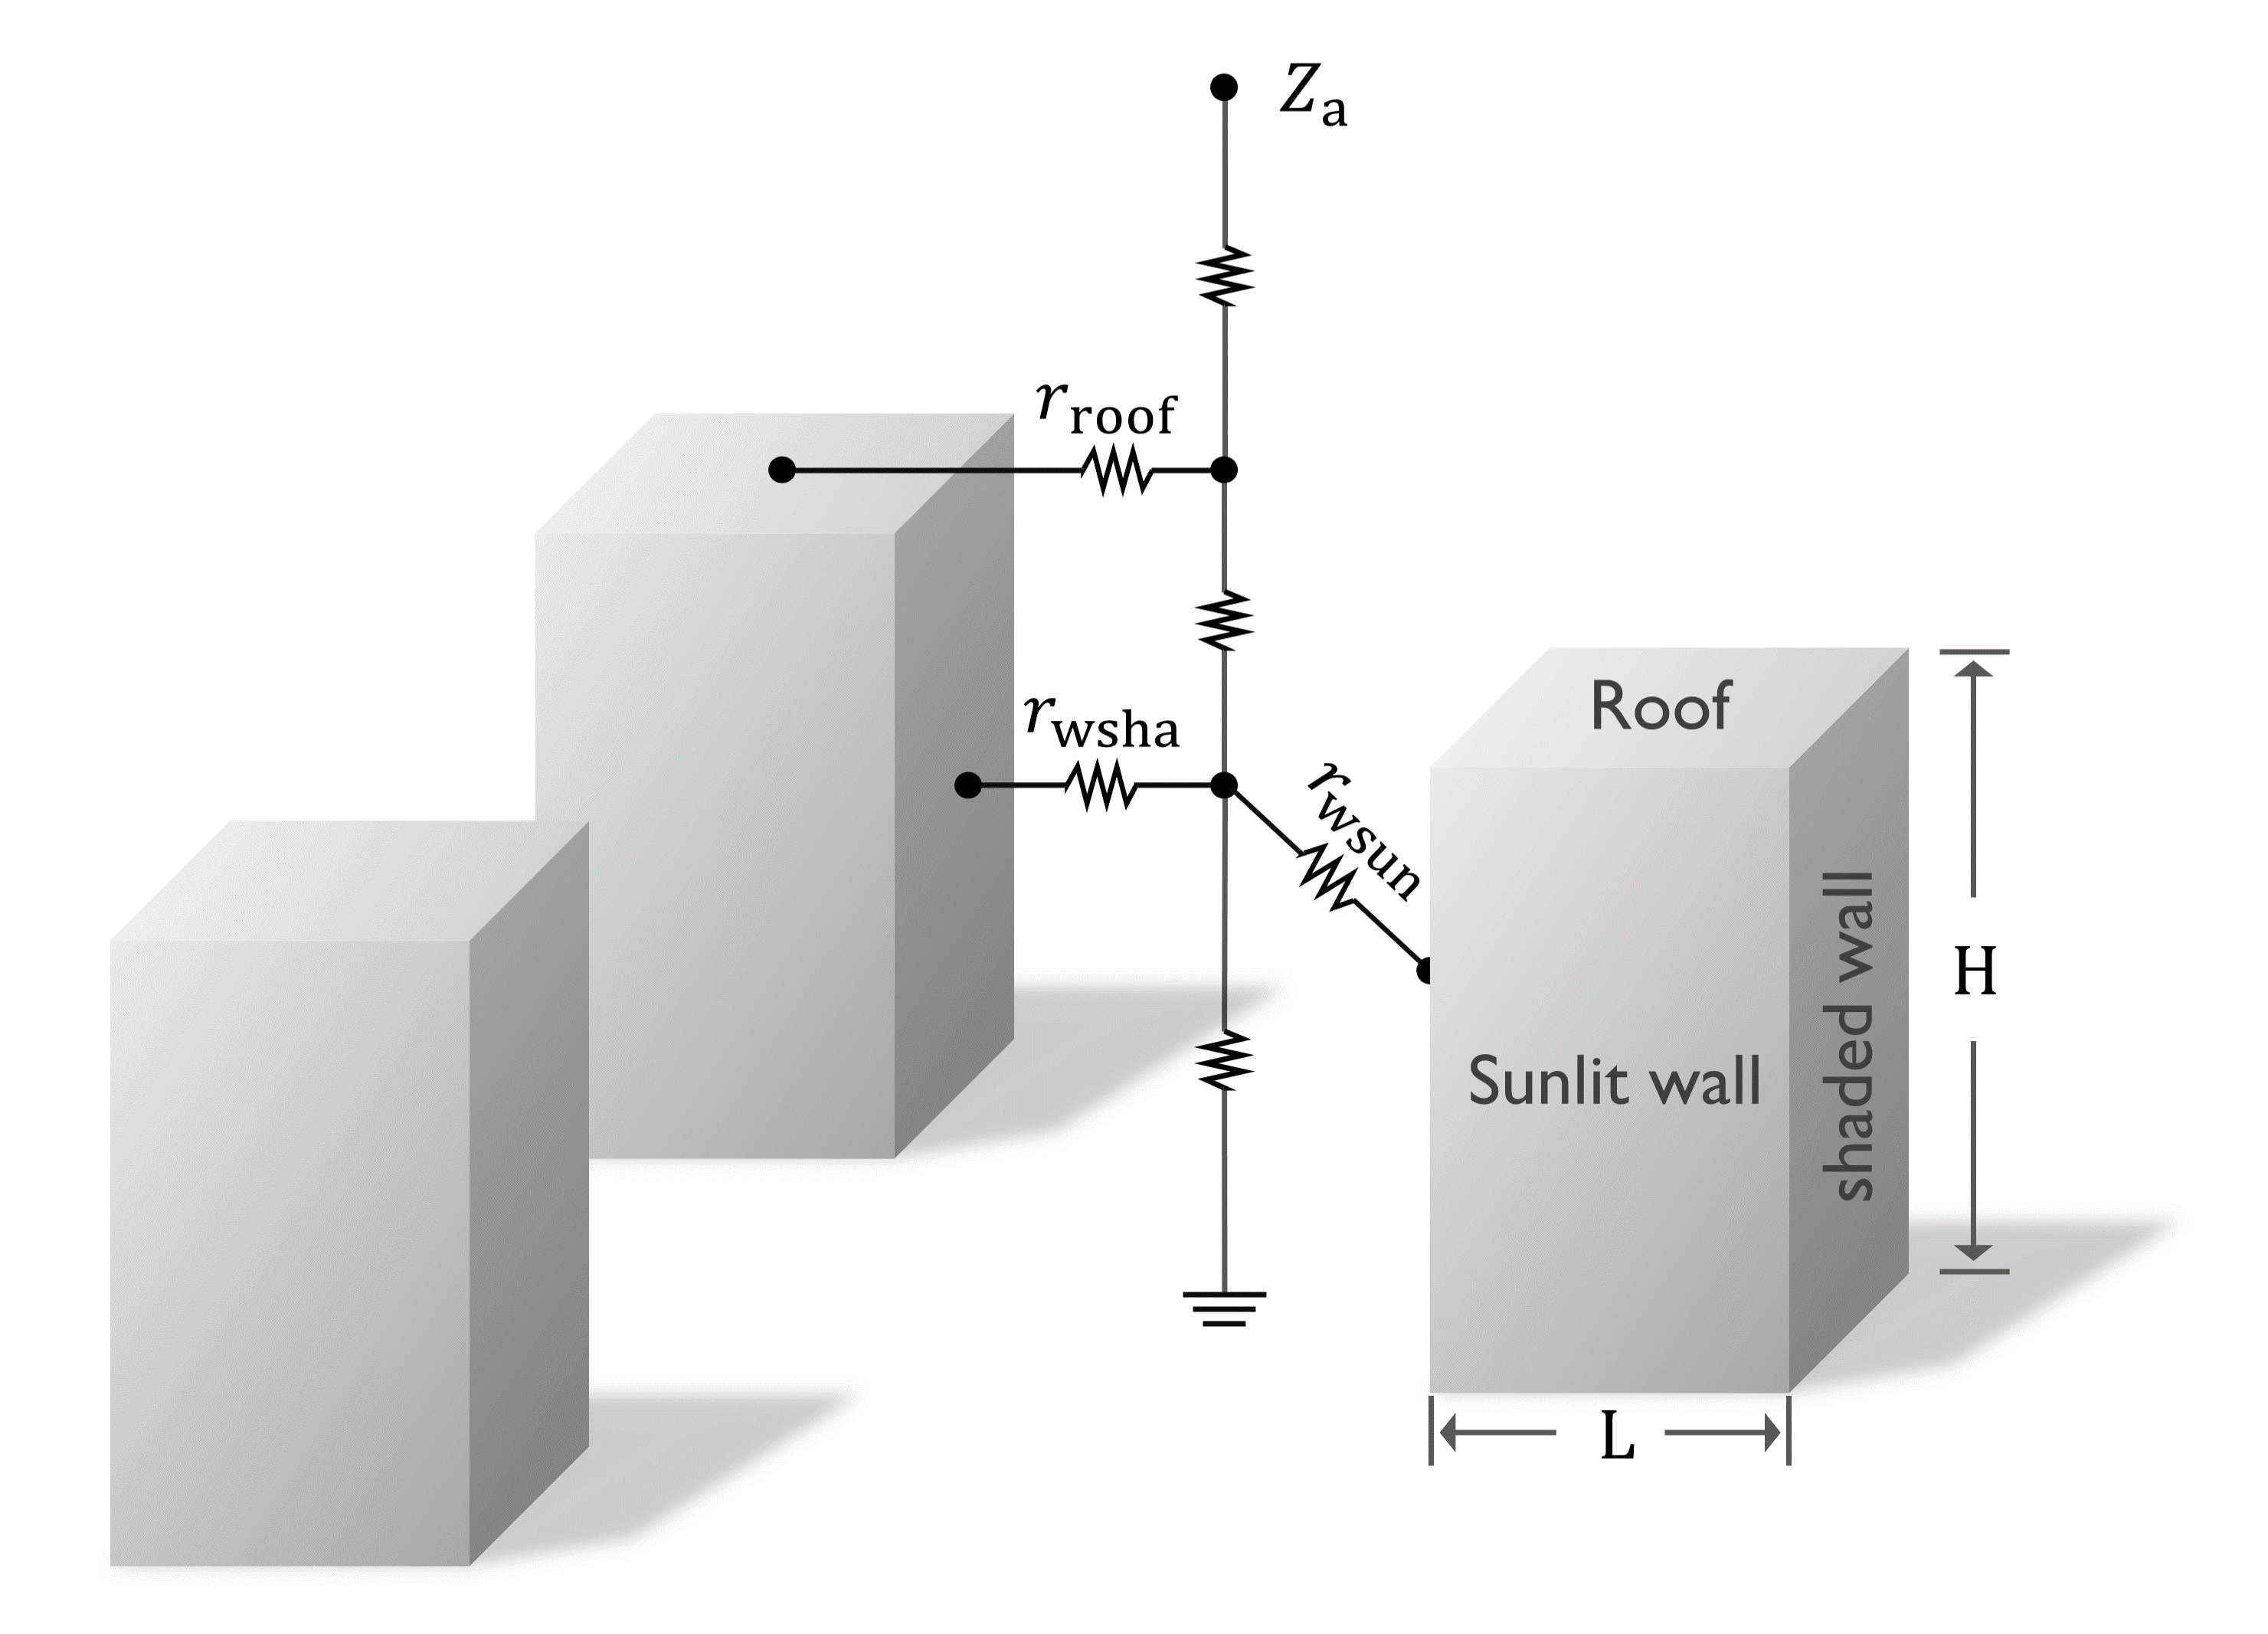
\includegraphics[width=0.75\textwidth]{Figures/城市模式/CoLM城市模式无植被阻抗交换网络_v2.png}
    \caption{CoLM城市模式无植被覆盖时湍流交换阻抗网络示意图}
    \label{fig:无植被覆盖时城市湍流交换阻抗示意图}
  \end{figure}
}

以上为主要区别于三维植被湍流交换过程计算的部分,整个湍流交换计算阻抗网络如图~\ref{fig:无植被覆盖时城市湍流交换阻抗示意图} 所示。
湍流交换计算过程与三维植被湍流交换方案类似,先通过相似性理论计算屋顶高度风速和湍流交换系数;然后根据指数衰减假设,参考三维植被湍流交换方案~\citep{dai2019different},根据公式(\ref{uz})和(\ref{Kz})计算风速和湍流交换系数在城市冠层内部剖面。屋顶的等效风速即为H高度时的风速,墙面的等效风速为H到地面的平均风速,通过风速剖面积分计算得到。同理,屋顶与墙面等效交换高度之间的动力学交换阻抗,以及墙面等效交换高度与地面之间的动力学阻抗$r_{\mathrm {d}}$均是通过对交换系数剖面积分计算得到(公式(\ref{r_d1}))。
同多层植被湍流交换计算一样,对上图所示的屋顶和墙面等效交换高度建立感热和潜热通量守恒方程,迭代求解其高度处的空气温度、湿度以及相似性理论交换长度(即空气不稳定程度)。

%感热通量
湍流交换过程在迭代计算时,需要求解城市建筑屋顶(第三层)、墙面(第二层)等效交换高度的温度(比湿) $T_3$($q_3$)与$T_2$($q_2$),以计算不同城市表面的湍流通量交换,在不考虑城市植被时,只存在地面(透水面$\rm gper$与不透水面$\rm gimp$)、阳面墙($\rm wsun$)、阴面墙($\rm wsha$)以及屋顶($\rm roof$)的交换过程,其中地面、墙体均在第二层交换,屋顶则在第三层交换,如图~\ref{fig:无植被覆盖时城市湍流交换阻抗示意图} 所示,在多层湍流交换方案中,层与层之间的通量交换保持平衡,通过建立不同层的通量交换方程即可求解$T_3$($q_3$)与$T_2$($q_2$),进而计算得到不同表面的感热/潜热通量。

对于感热而言,在不考虑城市植被时,其不同层的感热通量$H$可表达为:
\begin{equation}\label{2lays_noveg_H_layer2}
  H_{2} = H_{\mathrm{g}}
\end{equation}
%
\begin{equation}\label{2lays_noveg_H_layer3}
  H_{3} = H_{2} + H_{\mathrm{wsun}} + H_{\mathrm{wsha}} = \frac{\rho _{\rm a} C_{\mathrm a} \left( T_{2} - T_{3} \right)}{r_{\mathrm{d3}}}
\end{equation}
%
\begin{equation}\label{2lays_noveg_H}
  H = H_{3} + H_{\mathrm{roof}} = \frac{\rho _{\rm a} C_{\mathrm a} \left( T_{3} - T_{\rm a} \right)}{r_{\mathrm{ah}}}
\end{equation}
其中,$H_2$、$H_3$和$H$分别表示地面与第二层、第二层与第三层以及第三层与参考高度的感热通量交换,$H_{\mathrm{g}}$、$H_{\mathrm{wsun}}$、$H_{\mathrm{wsha}}$、$H_{\mathrm{roof}}$分别为地面、阳面墙、阴面墙以及屋顶的感热通量,其各自的表达式分别为:
\begin{equation}\label{urban_noveg_Hg}
  H_{\mathrm{g}} = \frac{\rho _{\rm a} C_{\mathrm a} \left( T_{\mathrm{g}} - T_{2} \right) \cdot f_{\mathrm{g}}}{r_{\mathrm{d2}}}
\end{equation}
%
\begin{equation}
  H_{\mathrm{wsun}} = \frac{\rho  _{\rm a} C_{\mathrm a} \left( T_{\mathrm{wsun}} - T_{2} \right) \cdot f_{\mathrm{wsun}}}{r_{\mathrm{wsun}}}
\end{equation}
%
\begin{equation}
  H_{\mathrm{wsha}} = \frac{\rho _{\rm a} C_{\mathrm a} \left( T_{\mathrm{wsha}} - T_{2} \right) \cdot f_{\mathrm{wsha}}}{r_{\mathrm{wsha}}}
\end{equation}
%
\begin{equation}\label{urban_noveg_Hroof}
  H_{\mathrm{roof}} = \frac{\rho _{\rm a} C_{\mathrm a} \left( T_{\mathrm{roof}} - T_{3} \right) \cdot f_{\mathrm{roof}}}{r_{\mathrm{roof}}}
\end{equation}
$T_2$和$T_3$分别表示第二层和第三层空气温度,$T_{\mathrm{g}}$为透水面与不透水面温度加权得到的平均温度,$r$为空气动力学阻抗,\allowbreak $f_{\mathrm{roof}}$,\allowbreak  $f_{\mathrm{wsun}}$,\allowbreak  $f_{\mathrm{wsha}}$分表代表屋顶、阳面墙以及阴面墙覆盖比例($f_{\mathrm{wsun}},f_{\mathrm{wsha}}$应包含乘积因子$4{\rm HL} \cdot f_{\rm b}$,为简化计算式表达形式,下面均省略)。$f_{\mathrm{g}}$则为除去建筑覆盖外的路面占比(包含透水面$f_{\mathrm{gper}}$以及不透水面$f_{\mathrm{gimp}}$),将以上表达式代回公式~\eqref{2lays_noveg_H_layer2}--\eqref{2lays_noveg_H},可得:
\begin{equation}
  \begin{split}
    & \frac{\rho _{\rm a} C_{\mathrm a} \left( T_{2} - T_{3} \right)}{r_{\mathrm{d3}}} = \\
    & \frac{\rho _{\rm a} C_{\mathrm a} \left( T_{\mathrm{g}} - T_{2} \right) \cdot f_{\mathrm{g}}}{r_{\mathrm{d2}}} + \frac{\rho _{\rm a} C_{\mathrm a} \left( T_{\mathrm{wsun}} - T_{2} \right) \cdot f_{\mathrm{wsun}}}{r_{\mathrm{wsun}}} + \frac{\rho _{\rm a} C_{\mathrm a} \left( T_{\mathrm{wsha}} - T_{2} \right) \cdot f_{\mathrm{wsha}}}{r_{\mathrm{wsha}}}
  \end{split}
\end{equation}
%
\begin{equation}
  \begin{split}
    \frac{\rho _{\rm a} C_{\mathrm a} \left( T_{3} - T_{\rm a} \right)}{r_{\mathrm{ah}}} =
    \frac{\rho _{\rm a} C_{\mathrm a} \left( T_{2} - T_{3} \right)}{r_{\mathrm{d3}}} + \frac{\rho _{\rm a} C_{\mathrm a} \left( T_{\mathrm{roof}} - T_{3} \right)\cdot f_{\mathrm{roof}}}{r_{\mathrm{roof}}}
  \end{split}
\end{equation}
进而得到关于$T_{2}$和$T_{3}$的二元一次方程:
\begin{equation}
%    \begin{split}
  T_{2} =
  \frac{\frac{T_{\mathrm{g}} \cdot f_{\mathrm{g}}}{r_{\mathrm{d2}}} + \frac{T_{\mathrm{wsun}} \cdot f_{\mathrm{wsun}}}{r_{\mathrm{wsun}}} + \frac{T_{\mathrm{wsha}} \cdot f_{\mathrm{wsha}}}{r_{\mathrm{wsha}}} + \frac{T_{3}}{r_{\mathrm{d3}}}}{\frac{1}{r_{\mathrm{d3}}} + \frac{f_{\mathrm{g}}}{r_{\mathrm{d2}}} + \frac{f_{\mathrm{wsun}}}{r_{\mathrm{wsun}}} + \frac{f_{\mathrm{wsha}}}{r_{\mathrm{wsha}}}}
%    \end{split}
\end{equation}
%
\begin{equation}\label{result_noveg_T_layer2}
  T_{3} = \frac{\frac{T_{2}}{r_{\mathrm{d3}}} + \frac{T_{\mathrm{roof}} \cdot f_{\mathrm{roof}}}{r_{\mathrm{roof}}} + \frac{T_{\rm a}}{r_{\mathrm{ah}}}}{\frac{1}{r_{\mathrm{ah}}} + \frac{1}{r_{\mathrm{d3}}} + \frac{f_{\mathrm{roof}}}{r_{\mathrm{roof}}}}
\end{equation}
求解该二元一次方程可得:
\begin{equation}
  \begin{split}
    % \hspace{-1cm}
    T_{2} =
    \frac{\frac{T_{\mathrm{g}} \cdot f_{\mathrm{g}}}{r_{\mathrm{d2}}} + \frac{T_{\mathrm{wsun}} \cdot f_{\mathrm{wsun}}}{r_{\mathrm{wsun}}} + \frac{T_{\mathrm{wsha}} \cdot f_{\mathrm{wsha}}}{r_{\mathrm{wsha}}} + a_{\mathrm{T}}}{c_{\mathrm{T}} \cdot \left( 1 - \frac{b_{\mathrm {T}} }{c_{\mathrm{T}} r_{\mathrm{d3}}} \right)}
  \end{split}
\end{equation}
%
其中:
\begin{equation}
  a_{\mathrm{T}} = \left(\frac{T_{\mathrm{roof}} \cdot f_{\mathrm{roof}}}{r_{\mathrm{roof}}} + \frac{T_{\rm a}}{r_{\mathrm{ah}}}\right) \cdot b_{\mathrm{T}}
\end{equation}
%
\begin{equation}
  b_{\mathrm{T}} = \frac{1}{r_{\mathrm{d3}} \cdot \left(\frac{1}{r_{\mathrm{ah}}} + \frac{1}{r_{\mathrm{d3}}} + \frac{f_{\mathrm{roof}}}{r_{\mathrm{roof}}} \right)}
\end{equation}
%
\begin{equation}
  c_{\mathrm{T}} = \frac{1}{r_{\mathrm{d3}}} + \frac{f_{\mathrm{g}}}{r_{\mathrm{d2}}} + \frac{f_{\mathrm{wsun}}}{r_{\mathrm{wsun}}} + \frac{f_{\mathrm{wsha}}}{r_{\mathrm{wsha}}}
\end{equation}
将$T_{\mathrm{2}}$代回公式~\eqref{result_noveg_T_layer2},即可求得$T_{3}$。

将求解得到的$T_{2}$与$T_{3}$分别代回公式~\eqref{urban_noveg_Hg}--\eqref{urban_noveg_Hroof},即可得到城市每个表面的感热通量。其后计算城市各表面温度并基于该温度变化对感热通量进行更新时,需要提供各表面感热对各自温度的变化率,各表面相应值分别计算为:
\begin{equation}
  \frac{\partial H_{\mathrm{g}}}{\partial T_{\mathrm{g}}} = \frac{\rho _{\rm a} C_{\mathrm a}}{r_{\mathrm{d2}}} \left(1-\frac{f_{\rm g}}{c_{\mathrm{T}} r_{\mathrm{d2}} \left(1-\frac{b_{\mathrm {T}} }{c_{\mathrm{T}} r_{\mathrm{d3}}}\right)}\right)
\end{equation}
%
\begin{equation}
  \frac{\partial H_{\mathrm{wsun}}}{\partial T_{\mathrm{wsun}}} = \frac{\rho _{\rm a} C_{\mathrm a}}{r_{\mathrm{wsun}}} \left(1-\frac{f_{\mathrm{wsun}}}{c_{\mathrm{T}} r_{\mathrm{wsun}} \left(1-\frac{b_{\mathrm {T}} }{c_{\mathrm{T}} r_{\mathrm{d2}}}\right)}\right)
\end{equation}
%
\begin{equation}
  \frac{\partial H_{\mathrm{wsha}}}{\partial T_{\mathrm{wsha}}} = \frac{\rho _{\rm a} C_{\mathrm a}}{r_{\mathrm{wsha}}} \left(1-\frac{f_{\mathrm{wsha}}}{c_{\mathrm{T}} r_{\mathrm{wsha}} \left(1-\frac{b_{\mathrm {T}} }{c_{\mathrm{T}} r_{\mathrm{d2}}}\right)}\right)
\end{equation}
%
\begin{equation}
  \frac{\partial H_{\mathrm{roof}}}{\partial T_{\mathrm{roof}}} = \frac{\rho _{\rm a} C_{\mathrm a}}{r_{\mathrm{roof}}} \left(1-\frac{f_{\mathrm{roof}} b_{\mathrm{T}}^2}{c_{\mathrm{T}} r_{\mathrm{roof}} \left(1-\frac{b_{\mathrm {T}} }{c_{\mathrm{T}} r_{\mathrm{d2}}}\right)}-\frac{f_{\mathrm{roof}}}{r_{\mathrm{roof}}\left(\frac{1}{r_{\mathrm{ah}}}+\frac{1}{r_{\mathrm{d2}}}+\frac{f_{\mathrm{roof}}}{r_{\mathrm{roof}}}\right)}\right)
\end{equation}

%潜热通量
潜热通量同样通过建立通量守恒方程分别求解第二层与第三层的比湿,即$q_2$与$q_3$。由于墙体不考虑积水情况,模式中未考虑墙体的潜热通量。因此,在第二层发生交换的仅有地面,由于考虑土壤阻抗,透水面与不透水面需要单独计算,在第三层发生交换的则仅有屋顶,对于不透水面与屋顶,仅考虑积水部分,所以对于建筑群落内部不同层次的潜热通量计算,在不考虑植被的情景下,其表达式为:
\begin{equation}\label{2lays_noveg_L_layer2}
  \lambda E_{\mathrm{2}} = \lambda E_{\mathrm{g}}
\end{equation}
%
\begin{equation}
  \lambda E_{3} = \lambda E_{2}
\end{equation}
%
\begin{equation}\label{2lays_noveg_L}
  \lambda E = \lambda E_{3} + \lambda E_{\mathrm{roof}}
\end{equation}
其中,$ E_{\mathrm{g}}$、$ E_{\mathrm{roof}}$分别为地面以及屋顶的水汽通量,其表达式分别为:
\begin{equation}\label{urban_noveg_Eg}
  E_{\mathrm{g}} = \frac{\rho _{\rm a} \left( q_{\mathrm{gper}}-q_{2} \right) \cdot f_{\mathrm{g}} \cdot f_{\mathrm{gper}}}{r_{\mathrm{d2}}+r_{\mathrm{ss}}} + \frac{\rho _{\rm a} \left( q_{\mathrm{gimp}}-q_{2} \right) \cdot f_{\mathrm{wet,gimp}} \cdot f_{\mathrm{g}} \cdot f_{\mathrm{gimp}}}{r_{\mathrm{d2}}}
\end{equation}
%
\begin{equation}\label{urban_noveg_Eroof}
  E_{\mathrm{roof}} = \frac{\rho _{\rm a} \left( q_{\mathrm{roof}}-q_{3}\right) \cdot f_{\mathrm{wet,roof}} \cdot f_{\mathrm{roof}}}{r_{\mathrm{roof}}}
\end{equation}
对于城市内的透水面,因为其本质是土壤,因此在计算其水汽通量时,考虑土壤阻抗($r_{\mathrm{ss}}$),因此透水面阻抗为第一层空气动力学阻抗与土壤阻抗之和($r_{\mathrm{d2}}$+$r_{\mathrm{ss}}$),$f_{\mathrm{wet}}$表示各表面干湿的比例,$q$为不同表面的比湿,将以上表达式代回公式~\eqref{2lays_noveg_L_layer2}--\eqref{2lays_noveg_L},可知:
\begin{equation}
  \frac{\rho _{\rm a} \left( q_{2}-q_{3}\right)}{r_{\mathrm{d3}}} =
  \frac{\rho _{\rm a} \left( q_{\mathrm{gper}}-q_{2}\right) \cdot f_{\mathrm{g}} \cdot f_{\mathrm{gper}}}{r_{\mathrm{d2}}+r_{\mathrm{ss}}} + \frac{\rho _{\rm a} \left( q_{\mathrm{gimp}}-q_{\mathrm{2}} \right) \cdot f_{\mathrm{wet,gimp}} \cdot f_{\mathrm{g}} \cdot f_{\mathrm{gimp}}}{r_{\mathrm{d2}}}
\end{equation}
%
\begin{equation}
  \frac{\rho _{\rm a} \left( q_{3} - q_{\rm a}\right)}{r_{\mathrm{aw}}} = \frac{\rho _{\rm a} \left( q_{2} - q_{3}\right)}{r_{\mathrm{d3}}} + \frac{\rho _{\rm a} \left( q_{\mathrm{roof}}-q_{3}\right) \cdot f_{\mathrm{wet,roof}} \cdot f_{\mathrm{roof}}}{r_{\mathrm{roof}}}
\end{equation}
同样可得关于$q_{2}$以及$q_{3}$的二元一次方程:
\begin{equation}
  q_{2} = \\
  \frac{\frac{q_{\mathrm{gper}} \cdot f_{\mathrm{g}} \cdot f_{\mathrm{gper}}}{r_{\mathrm{d2}} + r_{\mathrm{ss}}} + \frac{q_{\mathrm{gimp}} \cdot f_{\mathrm{g}} \cdot f_{\mathrm{wet,gimp}} \cdot f_{\mathrm{gimp}}}{r_{\mathrm{d2}}} + \frac{q_{3}}{r_{\mathrm{d3}}}}{\frac{1}{r_{\mathrm{d3}}} + \frac{f_{\mathrm{g}} \cdot f_{\mathrm{gper}}}{r_{\mathrm{d2}} + r_{\mathrm{ss}}} + \frac{f_{\mathrm{wet,gimp}} \cdot f_{\mathrm{g}} \cdot f_{\mathrm{gimp}}}{r_{\mathrm{d2}}}}
\end{equation}
%
\begin{equation}\label{equ_2lays_noveg_Q_lay3}
  q_{3} = \frac{\frac{q_{2}}{r_{\mathrm{d3}}} + \frac{q_{\mathrm{roof}} \cdot f_{\mathrm{wet,roof}} \cdot f_{\mathrm{roof}}}{r_{\mathrm{roof}}} + \frac{q_{\rm a}}{r_{\mathrm{aw}}}}{\frac{1}{r_{\mathrm{aw}}} + \frac{1}{r_{\mathrm{d3}}} + \frac{f_{\mathrm{wet,roof}} \cdot f_{\mathrm{roof}}}{r_{\mathrm{roof}}}}
\end{equation}
求解可得:
\begin{equation}
  q_{2} = \\
  \frac{\frac{q_{\mathrm{gper}} \cdot f_{\mathrm{g}} \cdot f_{\mathrm{gper}}}{r_{\mathrm{d2}}+r_{\mathrm{ss}}} + \frac{q_{\mathrm{gimp}} \cdot f_{\mathrm{g}} \cdot f_{\mathrm{wet,gimp}} \cdot f_{\mathrm{gimp}}}{r_{\mathrm{d2}} } + a_{\mathrm{q}}}{c_{\mathrm{q}} \cdot \left( 1 - \frac{b_{\mathrm{q}}}{c_{\mathrm{q}} \cdot r_{\mathrm{d3}}}\right)}
\end{equation}
%
其中:
\begin{equation}
  a_{\mathrm{q}}= \left(\frac{q_{\mathrm{roof}} \cdot f_{\mathrm{wet,roof}} \cdot f_{\mathrm{roof}}}{r_{\mathrm{roof}}} + \frac{q_{\rm a}}{r_{\mathrm{aw}}}\right) \cdot b_{\mathrm{q}}
\end{equation}
%
\begin{equation}
  b_{\mathrm{q}} = \frac{1}{r_{\mathrm{d3}} \cdot \left( \frac{1}{r_{\mathrm{aw}}} + \frac{1}{r_{\mathrm{d3}}} + \frac{f_{\mathrm{wet,roof}} \cdot f_{\mathrm{roof}}}{r_{\mathrm{roof}}} \right)}
\end{equation}
%
\begin{equation}
  c_{\mathrm{q}} = \frac{1}{r_{\mathrm{d3}}}+\frac{f_{\rm g} \cdot f_{\mathrm{gper}}}{r_{\mathrm{d2}}+r_{\mathrm{ss}}} + \frac{f_{\mathrm{wet,gimp}} \cdot f_{\rm g} \cdot f_{\mathrm{gimp}}}{r_{\mathrm{d2}}}
\end{equation}
同理,将$q_{2}$代入公式~\eqref{equ_2lays_noveg_Q_lay3} 即可求得$q_{3}$。

将求解得到的$q_{2}$与$q_{3}$分别代回公式~\eqref{urban_noveg_Eg}--\eqref{urban_noveg_Eroof},即可得到城市每个表面的水汽通量,其后计算城市各表面温度并基于该温度变化对水汽通量进行更新时,同样需要提供各表面水汽通量对各自温度的变化率,计算为:
\begin{equation}
  \frac{\partial  E_{\mathrm{gper}}}{\partial T_{\mathrm{gper}}} = \frac{\rho _{\rm a}}{r_{\mathrm{d2}}+r_{\mathrm{ss}}} \frac{{\mathrm {d}} q_{\mathrm{gper}}}{{\mathrm {d}} T_{\mathrm{gper}}} \left(1-\frac{f_{\mathrm{g}}f_{\mathrm{gper}}}{c_{\mathrm{q}} \left(r_{\mathrm{d2}}+r_{\mathrm{ss}}\right) \left(1-\frac{b_{\mathrm{q}}}{c_{\mathrm{q}} r_{\mathrm{d3}}}\right)}\right)
\end{equation}
%
\begin{equation}
  \frac{\partial  E_{\mathrm{gimp}}}{\partial T_{\mathrm{gimp}}} = \frac{\rho _{\rm a} f_{\mathrm{wet,gimp}}}{r_{\mathrm{d2}}} \frac{{\mathrm {d}} q_{\mathrm{gimp}}}{{\mathrm {d}} T_{\mathrm{gimp}}} \left(1-\frac{f_{\mathrm{wet,gimp}} f_{\mathrm{g}} f_{\mathrm{gimp}}}{c_{\mathrm{q}} r_{\mathrm{d2}}\left(1-\frac{b_{\mathrm{q}}}{c_{\mathrm{q}} r_{\mathrm{d3}}}\right)}\right)
\end{equation}
%
\begin{equation}
  \begin{split}
    &\frac{\partial  E_{\mathrm{roof}}}{\partial T_{\mathrm{roof}}} = \\
    &\frac{\rho _{\rm a} f_{\mathrm{wet,roof}}}{r_{\mathrm{roof}}} \frac{{\mathrm {d}} q_{\mathrm{roof}}}{{\mathrm {d}} T_{\mathrm{roof}}}\left(1-\frac{f_{\mathrm{wet,roof}}f_{\mathrm{roof}} b_{\mathrm{q}}^2}{c_{\mathrm{q}} r_{\mathrm{roof}} \left(1-\frac{b_{\mathrm{q}}}{c_{\mathrm{q}} r_{\mathrm{d3}}}\right)}-\frac{f_{\mathrm{wet,roof}}f_{\mathrm{roof}}}{r_{\mathrm{roof}}\left(\frac{1}{r_{\mathrm{ah}}}+\frac{1}{r_{\mathrm{d3}}}+\frac{f_{\mathrm{wet,roof}} f_{\mathrm{roof}}}{r_{\mathrm{roof}}}\right)}\right)
  \end{split}
\end{equation}

\subsection{有植被覆盖时湍流交换过程}
\esubsection{With Vegetation}
\begin{mymdframed}{代码}
  本节对应的代码文件为\texttt{MOD\_Urban\_Flux.F90}中\texttt{UrbanVegFlux()}函数。
\end{mymdframed}

{
  \begin{figure}[htbp]
    \centering
    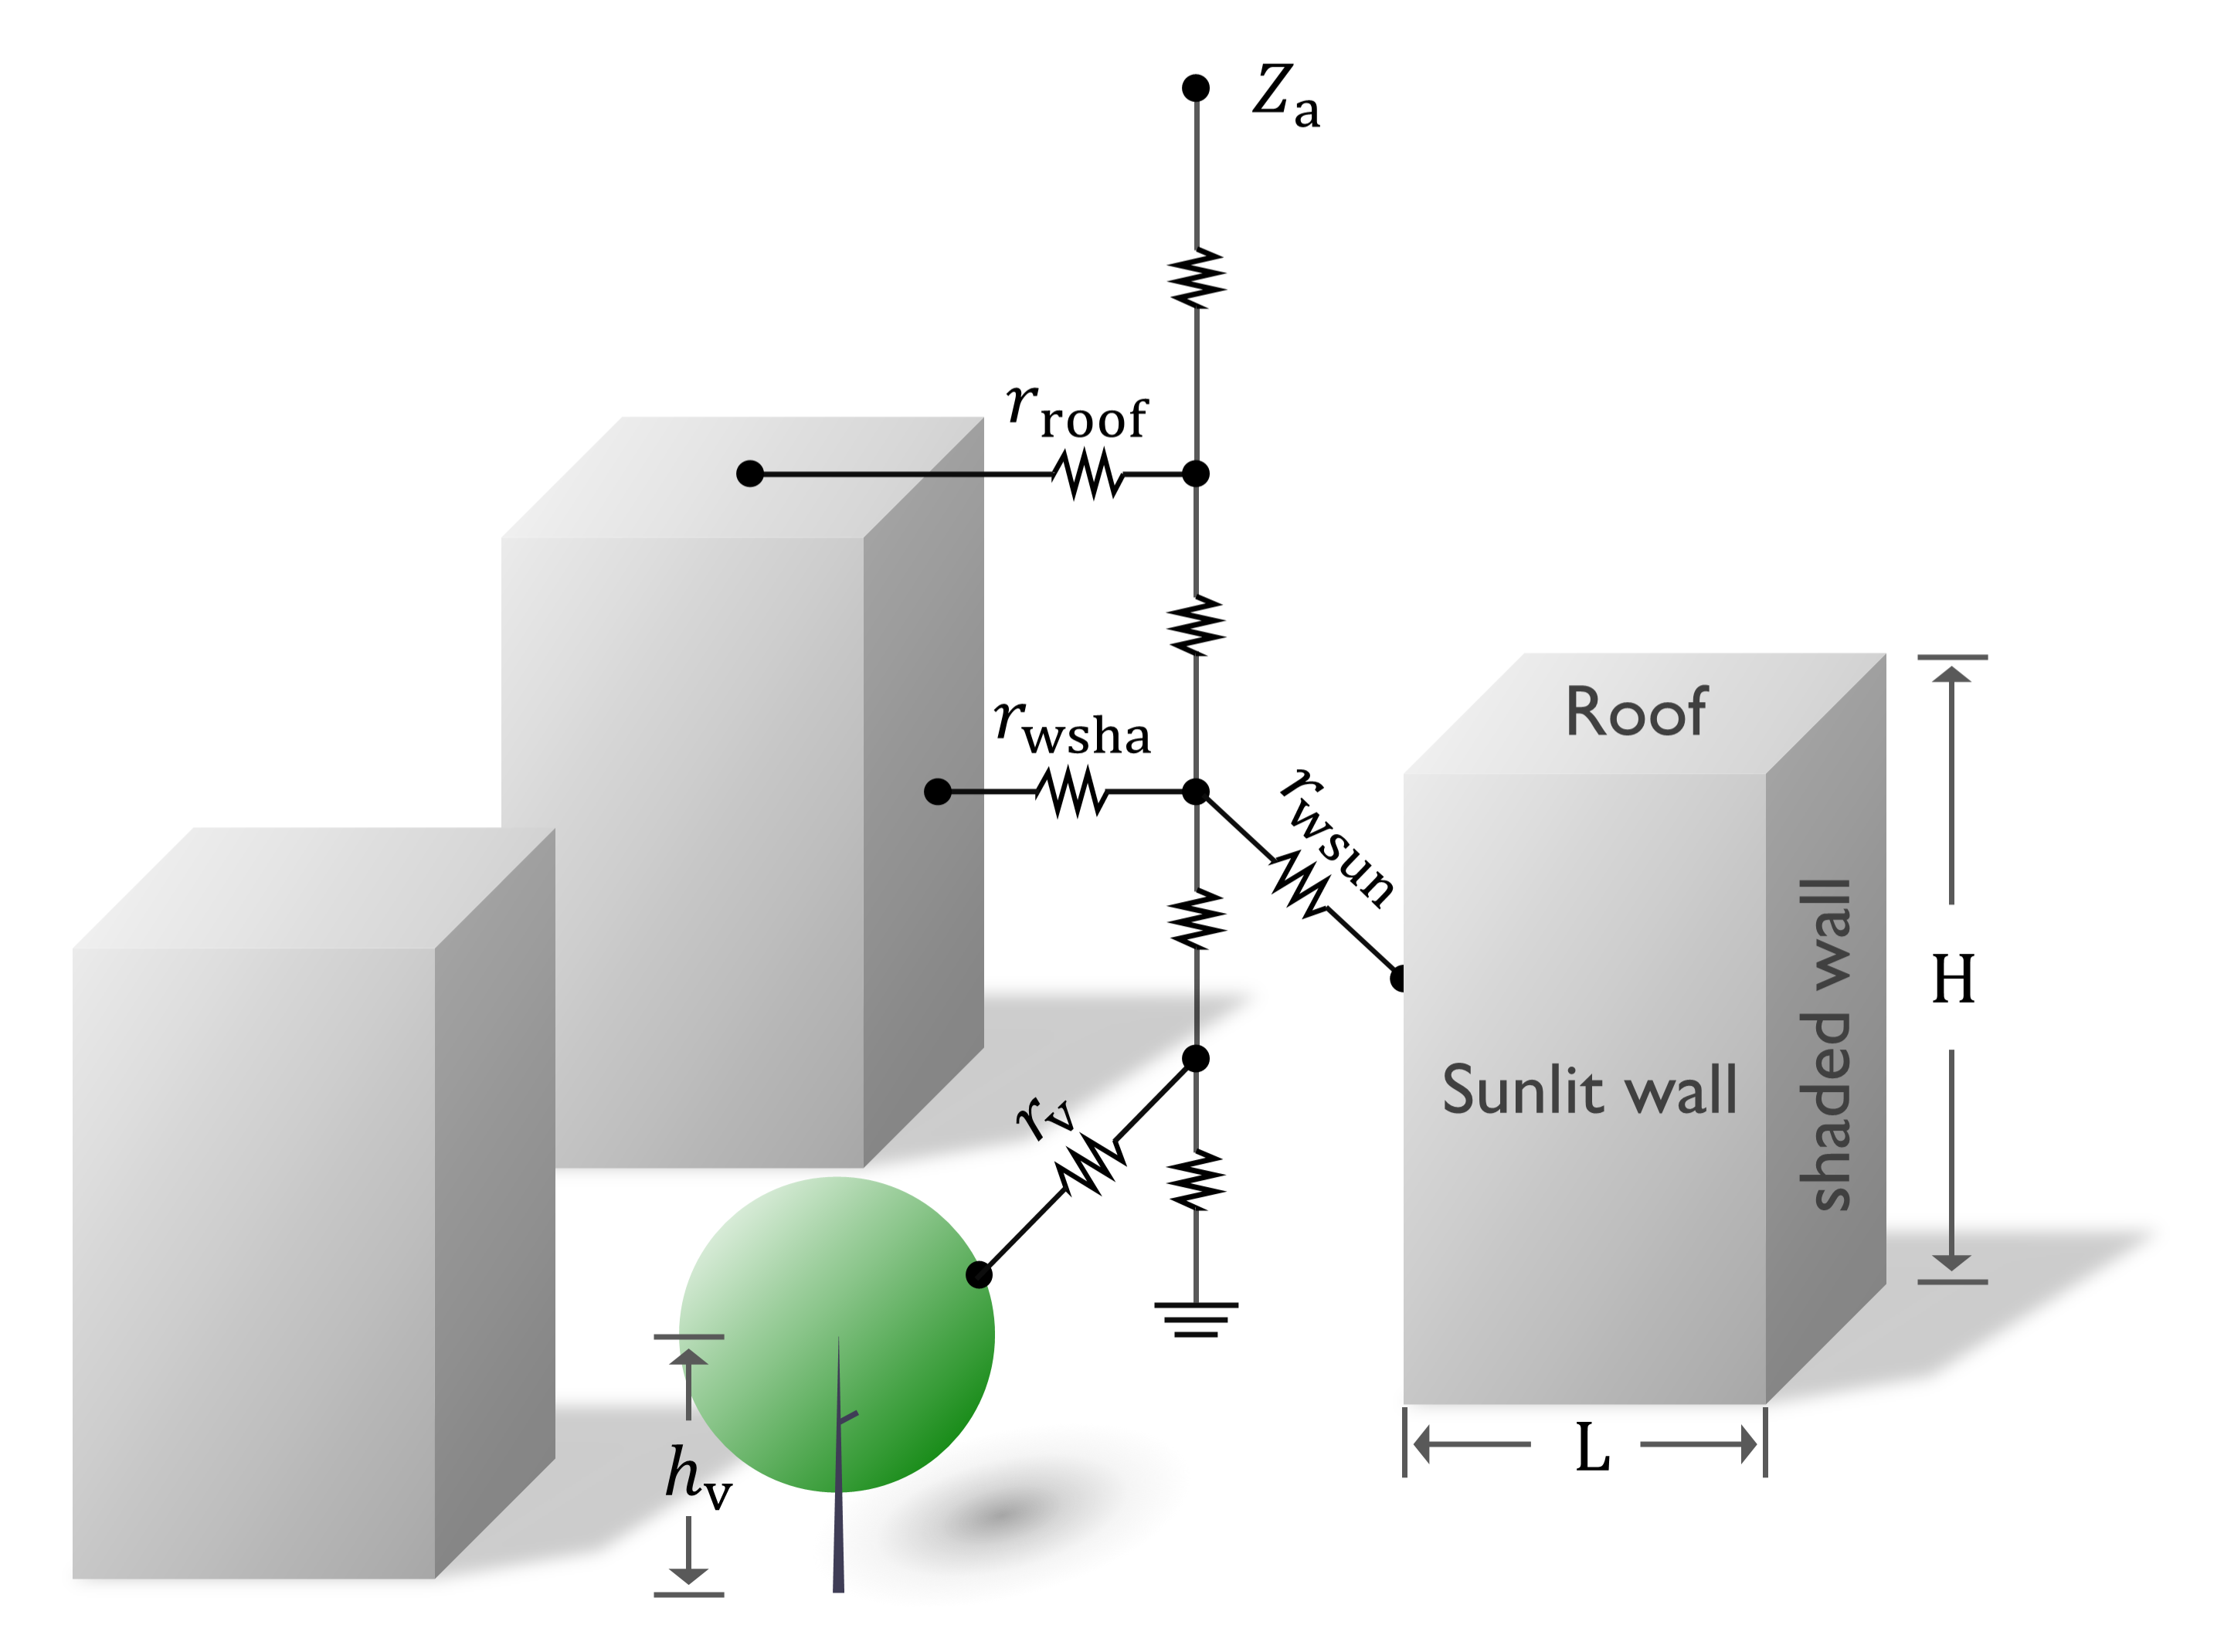
\includegraphics[width=0.75\textwidth]{Figures/城市模式/CoLM城市模式包含植被湍流交换阻抗网络_v2.png}
    \caption{CoLM城市模式有植被覆盖时湍流交换阻抗网络示意图}
    \label{fig:有植被覆盖时城市湍流交换阻抗示意图}
  \end{figure}
}
有植被覆盖时的湍流交换网络如图~\ref{fig:有植被覆盖时城市湍流交换阻抗示意图} 所示,其计算过程与无植被覆盖时类似,不同之处在于新增植被组分。因此,在建立通量守恒方程式时,需要考虑植被的感热、潜热交换,涉及到植被光合作用(蒸腾)和长波辐射吸收计算。
光合作用过程同自然植被光合作用过程,长波辐射吸收计算在章节~\ref{有植被覆盖时长波辐射传输} 已给出。
在实际计算过程中,可根据植被与建筑物高度差异,视情况分为两层或三层等效交换(三层时,即植被单独考虑为一层)。
整个过程也是迭代求解,但此时需要新增迭代求解变量叶片温度,其他过程同无植被覆盖时湍流交换过程。

\subsubsection{两层交换方案}\label{两层方案_植被}
因此,根据层与层之间通量交换守恒的原则,考虑城市植被时,其感热通量计算相较于无植被情景仅在第二层增加了植被的感热通量计算(当按两层阻抗网络计算时),即:
\begin{equation}
  H_{\mathrm{v}} = \frac{\rho _{\rm a} C_{\mathrm a} \left( T_{\mathrm{v}} - T_{2} \right) \cdot f_{\rm v}}{r_{\mathrm{v}}}
\end{equation}
此时,通量平衡方程变为:
\begin{equation}\label{2lays_veg_H_layer2}
  H_{2} = H_{\mathrm{g}}
\end{equation}
%
\begin{equation}\label{2lays_veg_H_layer3}
  H_{3} = H_{2} + H_{\mathrm{wsun}} + H_{\mathrm{wsha}} + H_{\mathrm{v}} = \frac{\rho _{\rm a} C_{\mathrm a} \left( T_{2} - T_{3} \right)}{r_{\mathrm{d3}}}
\end{equation}
%
\begin{equation}\label{2lays_veg_H}
  H = H_{3} + H_{\mathrm{roof}} = \frac{\rho _{\rm a} C_{\mathrm a} \left( T_{3} - T_{\rm a} \right)}{r_{\mathrm{ah}}}
\end{equation}
除植被感热通量$H_{\rm v}$以及植被覆盖比例$f_{\rm v}$外,上述公式其它各项含义与章节~\ref{无植被覆盖时湍流交换过程} 相同,将各表面的感热通量计算公式代回公式~\eqref{2lays_veg_H_layer2}--\eqref{2lays_veg_H},可得:
\begin{equation}
  \begin{split}
    & \frac{\rho _{\rm a} C_{\mathrm a} \left( T_{2} - T_{3} \right)}{r_{\mathrm{d3}}} = \\
    & \frac{\rho _{\rm a} C_{\mathrm a} \left( T_{\mathrm{g}} - T_{2} \right) \cdot f_{\mathrm{g}}}{r_{\mathrm{d2}}} + \frac{\rho _{\rm a} C_{\mathrm a} \left( T_{\mathrm{wsun}} - T_{2} \right) \cdot f_{\mathrm{wsun}}}{r_{\mathrm{wsun}}} + \frac{\rho _{\rm a} C_{\mathrm a} \left( T_{\mathrm{wsha}} - T_{2} \right) \cdot f_{\mathrm{wsha}}}{r_{\mathrm{wsha}}} +
    \\
    & \frac{\rho _{\rm a} C_{\mathrm a} \left( T_{\mathrm{v}} - T_{2} \right) \cdot f_{\rm v}}{r_{\mathrm{v}}}
  \end{split}
\end{equation}
%
\begin{equation}
  \begin{split}
    \frac{\rho _{\rm a} C_{\mathrm a} \left( T_{3} - T_{\rm a} \right)}{r_{\mathrm{ah}}} =
    \frac{\rho _{\rm a} C_{\mathrm a} \left( T_{2} - T_{3} \right)}{r_{\mathrm{d3}}} + \frac{\rho _{\rm a} C_{\mathrm a} \left( T_{\mathrm{roof}} - T_{3} \right)\cdot f_{\mathrm{roof}}}{r_{\mathrm{roof}}}
  \end{split}
\end{equation}
进而得到关于$T_{2}$和$T_{3}$的二元一次方程:
\begin{equation}
  \begin{split}
    T_{2} =
    \frac{\frac{T_{\mathrm{g}} \cdot f_{\mathrm{g}}}{r_{\mathrm{d2}}} + \frac{T_{\mathrm{wsun}} \cdot f_{\mathrm{wsun}}}{r_{\mathrm{wsun}}} + \frac{T_{\mathrm{wsha}} \cdot f_{\mathrm{wsha}}}{r_{\mathrm{wsha}}} + \frac{T_{\mathrm{v}} \cdot f_{\rm v}}{r_{\mathrm{v}}} + \frac{T_{\mathrm{3}}}{r_{\mathrm{d3}}}}{\frac{1}{r_{\mathrm{d3}}} + \frac{f_{\mathrm{g}}}{r_{\mathrm{d2}}} + \frac{f_{\mathrm{wsun}}}{r_{\mathrm{wsun}}} + \frac{f_{\mathrm{wsha}}}{r_{\mathrm{wsha}}} + \frac{f_{\rm v}}{r_{\mathrm{v}}}}
  \end{split}
\end{equation}
%
\begin{equation}\label{result_veg_T_layer3}
  T_{3} = \frac{\frac{T_{2}}{r_{\mathrm{d3}}} + \frac{T_{\mathrm{roof}} \cdot f_{\mathrm{roof}}}{r_{\mathrm{roof}}} + \frac{T_{\rm a}}{r_{\mathrm{ah}}}}{\frac{1}{r_{\mathrm{ah}}} + \frac{1}{r_{\mathrm{d3}}} + \frac{f_{\mathrm{roof}}}{r_{\mathrm{roof}}}}
\end{equation}
求解该二元一次方程可得:
\begin{equation}
  \begin{split}
    % \hspace{-1cm}
    T_{2} =
    \frac{\frac{T_{\mathrm{g}} \cdot f_{\mathrm{g}}}{r_{\mathrm{d2}}} + \frac{T_{\mathrm{wsun}} \cdot f_{\mathrm{wsun}}}{r_{\mathrm{wsun}}} + \frac{T_{\mathrm{wsha}} \cdot f_{\mathrm{wsha}}}{r_{\mathrm{wsha}}} + \frac{T_{\mathrm{v}} \cdot f_{\mathrm{v}}}{r_{\mathrm{v}}} + a_{\mathrm{T}}}{c_{\mathrm{T}} \cdot \left( 1 - \frac{b_{\mathrm {T}} }{c_{\mathrm{T}} r_{\mathrm{d3}}} \right)}
  \end{split}
\end{equation}
%
其中:
\begin{equation}
  a_{\mathrm{T}} = \left(\frac{T_{\mathrm{roof}} \cdot f_{\mathrm{roof}}}{r_{\mathrm{roof}}} + \frac{T_{\rm a}}{r_{\mathrm{ah}}}\right) \cdot b_{\mathrm{T}}
\end{equation}
%
\begin{equation}
  b_{\mathrm{T}} = \frac{1}{r_{\mathrm{d3}} \cdot \left(\frac{1}{r_{\mathrm{ah}}} + \frac{1}{r_{\mathrm{d3}}} + \frac{f_{\mathrm{roof}}}{r_{\mathrm{roof}}} \right)}
\end{equation}
%
\begin{equation}
  c_{\mathrm{T}} = \frac{1}{r_{\mathrm{d3}}} + \frac{f_{\mathrm{g}}}{r_{\mathrm{d2}}} + \frac{f_{\mathrm{wsun}}}{r_{\mathrm{wsun}}} + \frac{f_{\mathrm{wsha}}}{r_{\mathrm{wsha}}} + \frac{f_{\rm v}}{r_{\mathrm{v}}}
\end{equation}
将$T_{2}$代回公式~\eqref{result_veg_T_layer3},即可求得$T_{3}$。

将求解得到的$T_{2}$与$T_{3}$分别代回各表面的通量表达式,即可得到城市每个表面的感热通量,其后计算城市各表面温度并基于该温度变化对感热通量进行更新时,需要提供各表面感热对各自温度的变化率,各表面分别计算为:
\begin{equation}
  \frac{\partial H_{\mathrm{g}}}{\partial T_{\mathrm{g}}} = \frac{\rho _{\rm a} C_{\mathrm a}}{r_{\mathrm{d2}}} \left(1-\frac{f_{\rm g}}{c_{\mathrm{T}} r_{\mathrm{d2}} \left(1-\frac{b_{\mathrm {T}} }{c_{\mathrm{T}} r_{\mathrm{d3}}}\right)}\right)
\end{equation}
%
\begin{equation}
  \frac{\partial H_{\mathrm{wsun}}}{\partial T_{\mathrm{wsun}}} = \frac{\rho _{\rm a} C_{\mathrm a}}{r_{\mathrm{wsun}}} \left(1-\frac{f_{\mathrm{wsun}}}{c_{\mathrm{T}} r_{\mathrm{wsun}} \left(1-\frac{b_{\mathrm {T}} }{c_{\mathrm{T}} r_{\mathrm{d3}}}\right)}\right)
\end{equation}
%
\begin{equation}
  \frac{\partial H_{\mathrm{wsha}}}{\partial T_{\mathrm{wsha}}} = \frac{\rho _{\rm a} C_{\mathrm a}}{r_{\mathrm{wsha}}} \left(1-\frac{f_{\mathrm{wsha}}}{c_{\mathrm{T}} r_{\mathrm{wsha}} \left(1-\frac{b_{\mathrm {T}} }{c_{\mathrm{T}} r_{\mathrm{d3}}}\right)}\right)
\end{equation}
%
\begin{equation}
  \frac{\partial H_{\mathrm{v}}}{\partial T_{\mathrm{v}}} = \frac{\rho _{\rm a} C_{\mathrm a}}{r_{\mathrm{v}}} \left(1-\frac{f_{\mathrm{v}}}{c_{\mathrm{H}} r_{\mathrm{v}} \left(1-\frac{b_{\mathrm {T}} }{c_{\mathrm{T}} r_{\mathrm{d3}}}\right)}\right)
\end{equation}
%
\begin{equation}
  \frac{\partial H_{\mathrm{roof}}}{\partial T_{\mathrm{roof}}} = \frac{\rho _{\rm a} C_{\mathrm a}}{r_{\mathrm{roof}}} \left(1-\frac{f_{\mathrm{roof}} b_{\mathrm{T}}^2}{c_{\mathrm{T}} r_{\mathrm{roof}} \left(1-\frac{b_{\mathrm {T}} }{c_{\mathrm{T}} r_{\mathrm{d3}}}\right)}-\frac{f_{\mathrm{roof}}}{r_{\mathrm{roof}}\left(\frac{1}{r_{\mathrm{ah}}}+\frac{1}{r_{\mathrm{d3}}}+\frac{f_{\mathrm{roof}}}{r_{\mathrm{roof}}}\right)}\right)
\end{equation}

同样,对于潜热通量,相比章节~\ref{无植被覆盖时湍流交换过程},仅需要第二层加入植被的潜热通量计算,即:
\begin{equation}
  \lambda E_{\mathrm{v}} = \frac{\rho _{\rm a} \left( q_{\mathrm{v}}-q_{2}\right) \cdot f_{\rm v}}{r_{\mathrm{v}}}
\end{equation}
$r_{\rm v}$为植被与空气之间水汽交换总阻抗,是叶片边界层阻抗以及气孔阻抗之和($r_{\mathrm{b}}$+$r_{\mathrm{s}}$),此时,通量平衡方程可表达为:
\begin{equation}\label{2lays_veg_L_layer2}
  \lambda E_{2} = \lambda E_{\mathrm{g}}
\end{equation}
%
\begin{equation}
  \lambda E_{3} = \lambda E_{2} + \lambda E_{\mathrm{v}}
\end{equation}
%
\begin{equation}\label{2lays_veg_L}
  \lambda E = \lambda E_{3} + \lambda E_{\mathrm{roof}}
\end{equation}
其中,$\lambda E_{\mathrm{v}}$、$f_{\rm v}$分别为植被的潜热通量以及覆盖比例,上述公式其余各项含义同章节~\ref{无植被覆盖时湍流交换过程},将各表面通量的表达式代回公式~\eqref{2lays_veg_L_layer2}--\eqref{2lays_veg_L},可知:
\begin{equation}
  \begin{split}
    & \frac{\rho _{\rm a} \left( q_{2}-q_{3}\right)}{r_{\mathrm{d3}}} = \\
    & \frac{\rho _{\rm a} \left( q_{\mathrm{gper}}-q_{\mathrm{2}}\right) \cdot f_{\mathrm{g}} \cdot f_{\mathrm{gper}}}{r_{\mathrm{d2}}+r_{\mathrm{ss}}} + \frac{\rho _{\rm a} \left( q_{\mathrm{gimp}}-q_{2} \right) \cdot f_{\mathrm{wet,gimp}} \cdot f_{\mathrm{g}} \cdot f_{\mathrm{gimp}}}{r_{\mathrm{d2}}} + \frac{\rho _{\rm a} \left( q_{\mathrm{v}}-q_{2}\right) \cdot f_{\rm v}}{r_{\mathrm{v}}}
  \end{split}
\end{equation}
%
\begin{equation}
  \frac{\rho _{\rm a} \left( q_{3} - q_{\rm a}\right)}{r_{\mathrm{aw}}} = \frac{\rho _{\rm a} \left( q_{2} - q_{3}\right)}{r_{\mathrm{d3}}} + \frac{\rho _{\rm a} \left( q_{\mathrm{roof}}-q_{3}\right) \cdot f_{\mathrm{wet,roof}} \cdot f_{\mathrm{roof}}}{r_{\mathrm{roof}}}
\end{equation}
同样可得关于$q_{3}$以及$q_{3}$的二元一次方程:
\begin{equation}
  q_{2} = \\
  \frac{\frac{q_{\mathrm{gper}} \cdot f_{\mathrm{g}} \cdot f_{\mathrm{gper}}}{r_{\mathrm{d2}} + r_{\mathrm{ss}}} + \frac{q_{\mathrm{gimp}} \cdot f_{\mathrm{g}} \cdot f_{\mathrm{wet,gimp}} \cdot f_{\mathrm{gimp}}}{r_{\mathrm{d2}}} + \frac{q_{\mathrm{v}} \cdot f_{\rm v}}{r_{\mathrm{v}}} + \frac{q_{3}}{r_{\mathrm{d3}}}}{\frac{1}{r_{\mathrm{d3}}} + \frac{f_{\mathrm{g}} \cdot f_{\mathrm{gper}}}{r_{\mathrm{d2}} + r_{\mathrm{ss}}} + \frac{f_{\mathrm{wet,gimp}} \cdot f_{\mathrm{g}} \cdot f_{\mathrm{gimp}}}{r_{\mathrm{d2}}}+\frac{f_{\rm v}}{r_{\mathrm{v}}}}
\end{equation}
%
\begin{equation}\label{equ_2lays_veg_Q_lay3}
  q_{3} = \frac{\frac{q_{2}}{r_{\mathrm{d3}}} + \frac{q_{\mathrm{roof}} \cdot f_{\mathrm{wet,roof}} \cdot f_{\mathrm{roof}}}{r_{\mathrm{roof}}} + \frac{q_{\rm a}}{r_{\mathrm{aw}}}}{\frac{1}{r_{\mathrm{aw}}} + \frac{1}{r_{\mathrm{d3}}} + \frac{f_{\mathrm{wet,roof}} \cdot f_{\mathrm{roof}}}{r_{\mathrm{roof}}}}
\end{equation}
求解可得:
\begin{equation}
  q_{2} = \\
  \frac{\frac{q_{\mathrm{gper}} \cdot f_{\mathrm{g}} \cdot f_{\mathrm{gper}}}{r_{\mathrm{d1}}+r_{\mathrm{ss}}} + \frac{q_{\mathrm{gimp}} \cdot f_{\mathrm{g}} \cdot f_{\mathrm{wet,gimp}} \cdot f_{\mathrm{gimp}}}{r_{\mathrm{d3}} } + \frac{q_{\mathrm{v}} \cdot f_{\rm v}}{r_{\mathrm{v}}} + a_{\mathrm{q}}}{c_{\mathrm{q}} \cdot \left( 1 - \frac{b_{\mathrm{q}}}{c_{\mathrm{q}} \cdot r_{\mathrm{d3}}}\right)}
\end{equation}
%
其中:
\begin{equation}
  a_{\mathrm{q}}= \left(\frac{q_{\mathrm{roof}} \cdot f_{\mathrm{wet,roof}} \cdot f_{\mathrm{roof}}}{r_{\mathrm{roof}}} + \frac{q_{\rm a}}{r_{\mathrm{aw}}}\right) \cdot b_{\mathrm{q}}
\end{equation}
%
\begin{equation}
  b_{\mathrm{q}} = \frac{1}{r_{\mathrm{d3}} \cdot \left( \frac{1}{r_{\mathrm{aw}}} + \frac{1}{r_{\mathrm{d3}}} + \frac{f_{\mathrm{wet,roof}} \cdot f_{\mathrm{roof}}}{r_{\mathrm{roof}}} \right)}
\end{equation}
%
\begin{equation}
  c_{\mathrm{q}} = \frac{1}{r_{\mathrm{d3}}}+\frac{f_{\rm g} \cdot f_{\mathrm{gper}}}{r_{\mathrm{d2}}+r_{\mathrm{ss}}} + \frac{f_{\mathrm{wet,gimp}} \cdot f_{\rm g} \cdot f_{\mathrm{gimp}}}{r_{\mathrm{d2}}} + \frac{f_{\rm v}}{r_{\mathrm{v}}}
\end{equation}
同理,将$q_{2}$代入公式~\eqref{equ_2lays_veg_Q_lay3} 即可求得$q_{3}$。

其后计算城市各表面温度并基于该温度变化对水汽通量进行更新时,同样需要提供各表面水汽通量对各自温度的变化率,计算为:
\begin{equation}
  \frac{\partial  E_{\mathrm{gper}}}{\partial T_{\mathrm{gper}}} = \frac{\rho _{\rm a}}{r_{\mathrm{d2}}+r_{\mathrm{ss}}} \frac{{\mathrm {d}} q_{\mathrm{gper}}}{{\mathrm {d}} T_{\mathrm{gper}}} \left(1-\frac{f_{\mathrm{g}}f_{\mathrm{gper}}}{c_{\mathrm{q}} \left(r_{\mathrm{d2}}+r_{\mathrm{ss}}\right) \left(1-\frac{b_{\mathrm{q}}}{c_{\mathrm{q}} r_{\mathrm{d3}}}\right)}\right)
\end{equation}
%
\begin{equation}
  \frac{\partial  E_{\mathrm{gimp}}}{\partial T_{\mathrm{gimp}}} = \frac{\rho _{\rm a} f_{\mathrm{wet,gimp}}}{r_{\mathrm{d2}}} \frac{{\mathrm {d}} q_{\mathrm{gimp}}}{{\mathrm {d}} T_{\mathrm{gimp}}} \left(1-\frac{f_{\mathrm{wet,gimp}} f_{\mathrm{g}} f_{\mathrm{gimp}}}{c_{\mathrm{q}} r_{\mathrm{d3}}\left(1-\frac{b_{\mathrm{q}}}{c_{\mathrm{q}} r_{\mathrm{d3}}}\right)}\right)
\end{equation}
%
% \begin{equation}
% \frac{\partial  E_{\mathrm{v}}}{\partial T_{\mathrm{v}}} = \frac{\rho _{\rm a} C_{\mathrm a}}{r_{\mathrm{v}}} \frac{{\mathrm {d}} q_{\mathrm{v}}}{{\mathrm {d}} T_{\mathrm{v}}} \left(1-\frac{f_{\mathrm{v}}}{c_{\mathrm{q}} r_{\mathrm{v}}\left(1-\frac{b_{\mathrm{q}}}{c_{\mathrm{q}} r_{\mathrm{v}}}\right)}\right)
% \end{equation}
%
\begin{equation}
  \begin{split}
    & \frac{\partial  E_{\mathrm{roof}}}{\partial T_{\mathrm{roof}}} =\\
    &\frac{\rho _{\rm a} f_{\mathrm{wet,roof}}}{r_{\mathrm{roof}}} \frac{{\mathrm {d}} q_{\mathrm{roof}}}{{\mathrm {d}} T_{\mathrm{roof}}} \left(1-\frac{f_{\mathrm{wet,roof}}f_{\mathrm{roof}} b_{\mathrm{q}}^2}{c_{\mathrm{q}} r_{\mathrm{roof}} \left(1-\frac{b_{\mathrm{q}}}{c_{\mathrm{q}} r_{\mathrm{d3}}}\right)}-\frac{f_{\mathrm{wet,roof}}f_{\mathrm{roof}}}{r_{\mathrm{roof}}\left(\frac{1}{r_{\mathrm{ah}}}+\frac{1}{r_{\mathrm{d3}}}+\frac{f_{\mathrm{wet,roof}} f_{\mathrm{roof}}}{r_{\mathrm{roof}}}\right)}\right)
  \end{split}
\end{equation}
%
对于植被,其蒸腾与蒸发对应的各自温度变化率为:
%
\begin{equation}
  \frac{\partial  E_{\mathrm{tr}}}{\partial T_{\mathrm{v}}} = \frac{\rho _{\rm a} \delta \left(1-f_{\mathrm{wet}}\right){\rm LAI}} {r_{\mathrm{b}}+r_{\rm s}} \frac{{\mathrm {d}} q_{\mathrm{v}}}{{\mathrm {d}} T_{\mathrm{v}}} \left(1-\frac{f_{\mathrm{v}}}{c_{\mathrm{q}} r_{\mathrm{v}}\left(1-\frac{b_{\mathrm{q}}}{c_{\mathrm{q}} r_{\mathrm{v}}}\right)}\right)
\end{equation}
%
\begin{equation}
  \frac{\partial  E_{\mathrm{va}}}{\partial T_{\mathrm{v}}} = \frac{\rho _{\rm a} \left(1-\delta\left(1-f_{\mathrm{wet}}\right)\right)\left({\rm LAI} + {\rm SAI}\right)}{r_{\mathrm{b}}} \frac{{\mathrm {d}} q_{\mathrm{v}}}{{\mathrm {d}} T_{\mathrm{v}}} \left(1-\frac{f_{\mathrm{v}}}{c_{\mathrm{q}} r_{\mathrm{v}}\left(1-\frac{b_{\mathrm{q}}}{c_{\mathrm{q}} r_{\mathrm{v}}}\right)}\right)
\end{equation}
$\delta$为判断蒸腾是否发生的判别因子,其计算可参考公式~\eqref{delta_cal}。
%
%
\subsubsection{三层交换方案}
当建筑高度明显高于植被时,采用三层交换方案,此时,植被不再合并于第二层,而是单独在第一层交换,从而分别求解不同层的$T_{1}$($q_{1}$)、$T_{2}$($q_{2}$)与$T_{3}$($q_{3}$),以下为求解过程。
对于感热通量,不同层的感热通量$H$可表达为:
%
\begin{equation}
  \label{3lay_H1_veg}
  H_{1} = H_{\mathrm{g}}
\end{equation}
%
\begin{equation}
  H_{2} = H_{1}+H_{\mathrm{v}}
\end{equation}
%
\begin{equation}
  H_{3} = H_{2}+H_{\mathrm{wsun}}+H_{\mathrm{wsha}}
\end{equation}
%
\begin{equation}
  \label{3lay_H3_veg}
  H = H_{3}+H_{\mathrm{roof}}
\end{equation}
其各自表达式为:
\begin{equation}\label{urban_Hg_3_veg}
  H_{\mathrm{g}} = \frac{\rho _{\rm a} C_{\mathrm a} \left( T_{\mathrm{g}} - T_{1} \right) f_{\mathrm{g}}}{r_{\mathrm{d1}}}
\end{equation}
%
\begin{equation}
  H_{\mathrm{v}} = \frac{\rho _{\rm a} C_{\mathrm a} \left( T_{\mathrm{v}} - T_{1} \right) f_{\rm v}}{r_{\mathrm{v}}}
\end{equation}
%
\begin{equation}
  H_{\mathrm{wsun}} = \frac{\rho  _{\rm a} C_{\mathrm a} \left( T_{\mathrm{wsun}} - T_{2} \right) f_{\mathrm{wsun}}}{r_{\mathrm{wsun}}}
\end{equation}
%
\begin{equation}
  H_{\mathrm{wsha}} = \frac{\rho _{\rm a} C_{\mathrm a} \left( T_{\mathrm{wsha}} - T_{2} \right) f_{\mathrm{wsha}}}{r_{\mathrm{wsha}}}
\end{equation}
%
\begin{equation}\label{urban_Hroof_3_veg}
  H_{\mathrm{roof}} = \frac{\rho _{\rm a} C_{\mathrm a} \left( T_{\mathrm{roof}} - T_{\mathrm{3}} \right) f_{\mathrm{roof}}}{r_{\mathrm{roof}}}
\end{equation}
其各项含义两层方案相同(章节~\ref{两层方案_植被}),此处不再赘述,将以上表达式代回公式~\eqref{3lay_H1_veg}-~\eqref{3lay_H3_veg}可得:
%
\begin{equation}
  \frac{\rho _{\rm a} C_{\mathrm a} \left( T_{1} - T_{2} \right)}{r_{\mathrm{d3}}} = \frac{\rho _{\rm a} C_{\mathrm a} \left( T_{\mathrm{g}} - T_{1} \right) f_{\mathrm{g}}}{r_{\mathrm{d1}}} + \frac{\rho _{\rm a} C_{\mathrm a} \left( T_{\mathrm{v}} - T_{1} \right) f_{\rm v}}{r_{\mathrm{v}}}
\end{equation}
%
\begin{equation}
  \begin{split}
    & \frac{\rho _{\rm a} C_{\mathrm a} \left( T_{2} - T_{3} \right)}{r_{\mathrm{d3}}} = \\
    & \frac{\rho _{\rm a} C_{\mathrm a} \left( T_{1} - T_{2} \right) }{r_{\mathrm{d2}}} + \frac{\rho _{\rm a} C_{\mathrm a} \left( T_{\mathrm{wsun}} - T_{2} \right) \cdot f_{\mathrm{wsun}}}{r_{\mathrm{wsun}}} + \frac{\rho _{\rm a} C_{\mathrm a} \left( T_{\mathrm{wsha}} - T_{2} \right) \cdot f_{\mathrm{wsha}}}{r_{\mathrm{wsha}}}
  \end{split}
\end{equation}
%
\begin{equation}
  \begin{split}
    \frac{\rho _{\rm a} C_{\mathrm a} \left( T_{3} - T_{\rm a} \right)}{r_{\mathrm{ah}}} =
    \frac{\rho _{\rm a} C_{\mathrm a} \left( T_{2} - T_{3} \right)}{r_{\mathrm{d3}}} + \frac{\rho _{\rm a} C_{\mathrm a} \left( T_{\mathrm{roof}} - T_{3} \right)\cdot f_{\mathrm{roof}}}{r_{\mathrm{roof}}}
  \end{split}
\end{equation}
%
进而得到关于$T_{1}$、$T_{2}$与$T_{3}$的三元一次方程:
%
\begin{equation}
  \label{3lay_T1_veg}
  T_{1} =\frac{ \frac{T_{\mathrm{g}} f_{\mathrm{g}}}{r_{\mathrm{d1}}} + \frac{T_{\mathrm{v}} f_{\rm v}}{r_{\mathrm{v}}} + \frac{T_{2}}{r_{\mathrm{d2}}} }{\frac{1}{r_{\mathrm{d2}}} + \frac{f_{\mathrm{g}}}{r_{\mathrm{d1}}} + \frac{f_{\rm v}}{r_{\mathrm{v}}}}
\end{equation}
%
\begin{equation}
  T_{2} = \frac{\frac{T_{\mathrm{wsun}} f_{\mathrm{wsun}}}{r_{\mathrm{wsun}}} + \frac{T_{\mathrm{wsha}} f_{\mathrm{wsha}}}{r_{\mathrm{wsha}}} +  \frac{T_{1}}{r_{\mathrm{d2}}} + \frac{T_{3}}{r_{\mathrm{d3}}}}{\frac{1}{r_{\mathrm{d3}}} + \frac{1}{r_{\mathrm{d2}}} + \frac{f_{\mathrm{wsun}}}{r_{\mathrm{wsun}}} + \frac{f_{\mathrm{wsha}}}{r_{\mathrm{wsha}}}}
\end{equation}
%
\begin{equation}
  \label{3lay_T3_veg}
  T_{3} = \frac{\frac{T_{\mathrm{roof}} f_{\mathrm{roof}}}{r_{\mathrm{roof}}} + \frac{T_{2}}{r_{\mathrm{d3}}} + \frac{T_{\rm a}}{r_{\mathrm{ah}}}}{\frac{1}{r_{\mathrm{ah}}} + \frac{1}{r_{\mathrm{d3}}} + \frac{f_{\mathrm{roof}}}{r_{\mathrm{roof}}}}
\end{equation}
求解该方程可得:
\begin{equation}
  \begin{split}
    T_{2} = \frac{\frac{T_{\mathrm{wsun}} f_{\mathrm{wsun}}}{r_{\mathrm{wsun}}} + \frac{T_{\mathrm{wsha}} f_{\mathrm{wsha}}}{r_{\mathrm{wsha}}} + \left(\frac{T_{\mathrm{g}} f_{\mathrm{g}}}{r_{\mathrm{d1}}} + \frac{T_{\mathrm{v}} f_{\mathrm{v}}}{rv} \right)a_{\mathrm{T}} + \left(\frac{T_{\mathrm{roof}} f_{\mathrm{roof}}}{r_{\mathrm{roof}}} + \frac{T_{\mathrm{a}}}{r_{\mathrm{ah}}} \right)b_{\mathrm{T}}}{c_{\mathrm{T}} \left(1-\frac{a_{\mathrm{T}}}{c_{\mathrm{T}} r_{\mathrm{d2}}}-\frac{b_{\mathrm{T}}}{c_{\mathrm{T}} r_{\mathrm{d3}}}\right)}
  \end{split}
\end{equation}
其中:
\begin{equation}
  a_{\mathrm{T}} = \frac{1}{r_{\mathrm{d2}} \left(\frac{1}{r_{\mathrm{d2}}} + \frac{fg}{r_{\mathrm{d1}}} + \frac{f_{\mathrm{v}}}{r_{\mathrm{v}}} \right)}
\end{equation}
%
\begin{equation}
  b_{\mathrm{T}} = \frac{1}{r_{\mathrm{d3}} \left(\frac{1}{r_{\mathrm{ah}}} + \frac{1}{r_{\mathrm{d3}}} + \frac{f_{\mathrm{roof}}}{r_{\mathrm{roof}}} \right)}
\end{equation}
%
\begin{equation}
  c_{\mathrm{T}} = \frac{1}{r_{\mathrm{d3}}} + \frac{1}{r_{\mathrm{d2}}} + \frac{f_{\mathrm{wsun}}}{r_{\mathrm{wsun}}} + \frac{f_{\mathrm{wsha}}}{r_{\mathrm{wsha}}}
\end{equation}
将$T_{2}$分别代回公式~\eqref{3lay_T1_veg}、~\eqref{3lay_T3_veg},即可求得$T_{1}$与$T_{3}$。其后计算城市各表面温度并基于该温度变化对感热通量进行更新时,各表面感热对各自温度的变化率分别为:
\begin{equation}
  \frac{\partial H_{\mathrm{g}}}{\partial T_{\mathrm{g}}} = \frac{\rho _{\rm a} C_{\mathrm a}}{r_{\mathrm{d1}}} \left(1-\frac{f_{\rm g}}{r_{\mathrm{d1}} \left(\frac{1}{r_{\mathrm{d2}}}+\frac{f_{\rm g}}{r_{\mathrm{d1}}}+\frac{f_{\rm v}}{r_{\rm v}}\right)} - \frac{f_{\rm g} a_{\mathrm{T}}^2}{r_{\mathrm{d1}} c_{\mathrm{T}} \left(1-\frac{a_{\mathrm{T}}}{c_{\mathrm{T}} r_{\mathrm{d2}}}-\frac{b_{\mathrm{T}}}{c_{\mathrm{T}} r_{\mathrm{d3}}}\right)}\right)
\end{equation}
%
\begin{equation}
  \frac{\partial H_{\mathrm{wsun}}}{\partial T_{\mathrm{wsun}}} = \frac{\rho _{\rm a} C_{\mathrm a}}{r_{\mathrm{wsun}}} \left(1-\frac{f_{\mathrm{wsun}}}{c_{\mathrm{T}} r_{\mathrm{wsun}} \left(1-\frac{a_{\mathrm{T}}}{c_{\mathrm{T}} r_{\mathrm{d2}}}-\frac{b_{\mathrm{T}}}{c_{\mathrm{T}} r_{\mathrm{d3}}}\right)}\right)
\end{equation}
%
\begin{equation}
  \frac{\partial H_{\mathrm{wsha}}}{\partial T_{\mathrm{wsha}}} = \frac{\rho _{\rm a} C_{\mathrm a}}{r_{\mathrm{wsha}}} \left(1-\frac{f_{\mathrm{wsha}}}{c_{\mathrm{T}} r_{\mathrm{wsha}} \left(1-\frac{a_{\mathrm{T}}}{c_{\mathrm{T}} r_{\mathrm{d2}}}-\frac{b_{\mathrm{T}}}{c_{\mathrm{T}} r_{\mathrm{d3}}}\right)}\right)
\end{equation}
%
\begin{equation}
  \frac{\partial H_{\mathrm{v}}}{\partial T_{\mathrm{v}}} = \frac{\rho _{\rm a} C_{\mathrm a}}{r_{\mathrm{v}}} \left(1-\frac{f_{\rm v}}{r_{\mathrm{v}} \left(\frac{1}{r_{\mathrm{d2}}}+\frac{f_{\rm g}}{r_{\mathrm{d1}}}+\frac{f_{\rm v}}{r_{\rm v}}\right)} - \frac{f_{\rm v} a_{\mathrm{T}}^2}{r_{\mathrm{v}} c_{\mathrm{T}} \left(1-\frac{a_{\mathrm{T}}}{c_{\mathrm{T}} r_{\mathrm{d2}}}-\frac{b_{\mathrm{T}}}{c_{\mathrm{T}} r_{\mathrm{d3}}}\right)}\right)
\end{equation}
%
\begin{equation}
  \frac{\partial H_{\mathrm{roof}}}{\partial T_{\mathrm{roof}}} = \frac{\rho _{\rm a} C_{\mathrm a}}{r_{\mathrm{roof}}} \left(1-\frac{f_{\mathrm{roof}} b_{\mathrm{T}}^2}{c_{\mathrm{T}} r_{\mathrm{roof}} \left(1-\frac{a_{\mathrm{T}}}{c_{\mathrm{T}} r_{\mathrm{d2}}}-\frac{b_{\mathrm{T}}}{c_{\mathrm{T}} r_{\mathrm{d3}}}\right)}-\frac{f_{\mathrm{roof}}}{r_{\mathrm{roof}}\left(\frac{1}{r_{\mathrm{ah}}}+\frac{1}{r_{\mathrm{d3}}}+\frac{f_{\mathrm{roof}}}{r_{\mathrm{roof}}}\right)}\right)
\end{equation}
%-------------
%潜热通量
%-------------
对于潜热通量,其每一层的通量可表达为:
%
\begin{equation}\label{3lay_L1_veg}
  \lambda E_{1} = \lambda E_{\mathrm{g}}
\end{equation}
%
\begin{equation}
  \lambda E_{2} = \lambda E_{1} + \lambda E_{\mathrm{v}}
\end{equation}
%
\begin{equation}\label{3lay_L2_veg}
  \lambda E_{3} = \lambda E_{2}
\end{equation}
%
\begin{equation}\label{3lay_L3_veg}
  \lambda E = \lambda E_{3} + \lambda E_{\mathrm{roof}}
\end{equation}
其中,各个表面的水汽通量计算为:
\begin{equation}\label{3lay_Eg_veg}
  E_{\mathrm{g}} = \frac{\rho _{\rm a} \left( q_{\mathrm{gper}}-q_{1} \right) f_{\mathrm{g}} f_{\mathrm{gper}}}{r_{\mathrm{d1}}+r_{\mathrm{ss}}} + \frac{\rho _{\rm a} \left( q_{\mathrm{gimp}}-q_{1} \right) f_{\mathrm{wet,gimp}} f_{\mathrm{g}}  f_{\mathrm{gimp}}}{r_{\mathrm{d1}}}
\end{equation}
%
\begin{equation}
  E_{\mathrm{v}} = \frac{\rho _{\rm a} \left( q_{\mathrm{v}}-q_{1}\right) f_{\rm v}}{r_{\mathrm{v}}}
\end{equation}
%
\begin{equation}\label{3lay_Eroof_veg}
  E_{\mathrm{roof}} = \frac{\rho _{\rm a} \left( q_{\mathrm{roof}}-q_{3}\right) f_{\mathrm{wet,roof}} f_{\mathrm{roof}}}{r_{\mathrm{roof}}}
\end{equation}
其各项含义两层方案相同(章节~\ref{两层方案_植被}),此处不再赘述,将以上表达式代回公式~\eqref{3lay_L1_veg}-~\eqref{3lay_L3_veg}可得:
\begin{equation}
  \begin{split}
    & \frac{\rho _{\rm a} \left( q_{1}-q_{2}\right)}{r_{\mathrm{d2}}} = \\
    & \frac{\rho _{\rm a} \left( q_{\mathrm{gper}}-q_{1}\right) f_{\mathrm{g}} f_{\mathrm{gper}}}{r_{\mathrm{d1}}+r_{\mathrm{ss}}} + \frac{\rho _{\rm a} \left( q_{\mathrm{gimp}}-q_{1} \right) f_{\mathrm{wet,gimp}} f_{\mathrm{g}} f_{\mathrm{gimp}}}{r_{\mathrm{d1}}} + \frac{\rho _{\rm a} \left( q_{\mathrm{v}}-q_{1}\right) \cdot f_{\rm v}}{r_{\mathrm{v}}}
  \end{split}
\end{equation}
%
\begin{equation}
  \frac{\rho _{\rm a} \left( q_{2} - q_{3}\right)}{r_{\mathrm{d3}}} = \frac{\rho _{\rm a} \left( q_{1} - q_{2}\right)}{r_{2}}
\end{equation}
%
\begin{equation}
  \frac{\rho _{\rm a} \left( q_{3} - q_{\rm a}\right)}{r_{\mathrm{aw}}} = \frac{\rho _{\rm a} \left( q_{2} - q_{3}\right)}{r_{\mathrm{d3}}} + \frac{\rho _{\rm a} \left( q_{\mathrm{roof}}-q_{3}\right) f_{\mathrm{wet,roof}} f_{\mathrm{roof}}}{r_{\mathrm{roof}}}
\end{equation}
进而得到关于$q_{1}$、$q_{2}$与$q_{3}$的三元一次方程:
\begin{equation}
  \label{3lay_q1_veg}
  q_{1} = \frac{\frac{q_{\mathrm{gper}} f_{\mathrm{g}} f_{\mathrm{gper}}}{r_{\mathrm{d1}} + r_{\mathrm{ss}}} + \frac{q_{\mathrm{gimp}} f_{\mathrm{g}} f_{\mathrm{wet,gimp}} f_{\mathrm{gimp}}}{r_{\mathrm{d1}}} + \frac{q_{\mathrm{v}} f_{\rm v}}{r_{\mathrm{v}}} + \frac{q_{2}}{r_{\mathrm{d2}}}}{\left(\frac{1}{r_{\mathrm{d2}}} + \frac{f_{\mathrm{g}} f_{\mathrm{gper}}}{r_{\mathrm{d1}} + r_{\mathrm{ss}}} + \frac{f_{\mathrm{wet,gimp}} f_{\mathrm{g}} f_{\mathrm{gimp}}}{r_{\mathrm{d1}}}+\frac{f_{\rm v}}{r_{\mathrm{v}}}\right)}
\end{equation}
%
\begin{equation}
  q_{2} = \frac{\frac{q_{3}}{r_{\mathrm{d3}}} + \frac{q_{1}}{r_{\mathrm{d2}}}}{\frac{1}{r_{\mathrm{d3}}} + \frac{1}{r_{\mathrm{d2}}}}
\end{equation}
%
\begin{equation}
  \label{3lay_q3_veg}
  q_{3} = \frac{ \frac{q_{\mathrm{2}}}{r_{\mathrm{d3}}} + \frac{q_{\mathrm{roof}} f_{\mathrm{wet,roof}} f_{\mathrm{roof}}}{r_{\mathrm{roof}}} + \frac{q_{\rm a}}{r_{\mathrm{aw}}} }{ \frac{1}{r_{\mathrm{aw}}} + \frac{1}{r_{\mathrm{d3}}} + \frac{f_{\mathrm{wet,roof}} f_{\mathrm{roof}}}{r_{\mathrm{roof}}} }
\end{equation}
求解该方程可得:
\begin{equation}
  q_{2} = \\
  \frac{\left(\frac{q_{\mathrm{gper}} f_{\mathrm{g}} f_{\mathrm{gper}}}{r_{\mathrm{d1}}+r_{\mathrm{ss}}} + \frac{q_{\mathrm{gimp}} f_{\mathrm{g}} f_{\mathrm{wet,gimp}} f_{\mathrm{gimp}}}{r_{\mathrm{d1}}} + \frac{q_{\mathrm{v}} f_{\rm v}}{r_{\mathrm{v}}}\right)a_{\mathrm{q}} + \left(\frac{q_{\mathrm{roof}} f_{\mathrm{wet,roof}} f_{\mathrm{roof}}}{r_{\mathrm{roof}}} + \frac{q_{\rm a}}{r_{\mathrm{aw}}}\right)b_{\mathrm{q}} }{c_{\mathrm{q}} \left( 1 - \frac{a_{\mathrm{q}}}{c_{\mathrm{q}} r_{\mathrm{d2}}} - \frac{b_{\mathrm{q}}}{c_{\mathrm{q}} r_{\mathrm{d3}}} \right)}
\end{equation}
其中:
\begin{equation}
  a_{\mathrm{q}}= \frac{1}{r_{\mathrm{d2}} \left( \frac{1}{r_{\mathrm{d2}}} + \frac{f_{\mathrm{g}} f_{\mathrm{gper}}}{r_{\mathrm{d1}} + r_{\mathrm{ss}}} + \frac{f_{\mathrm{wet,gimp}} f_{\mathrm{g}} f_{\mathrm{gimp}}}{r_{\mathrm{d1}}}+\frac{f_{\rm v}}{r_{\mathrm{v}}} \right)}
\end{equation}
%
\begin{equation}
  b_{\mathrm{q}} = \frac{1}{r_{\mathrm{d3}} \left( \frac{1}{r_{\mathrm{aw}}} + \frac{1}{r_{\mathrm{d3}}} + \frac{f_{\mathrm{wet,roof}} f_{\mathrm{roof}}}{r_{\mathrm{roof}}} \right)}
\end{equation}
%
\begin{equation}
  c_{\mathrm{q}} = \frac{1}{r_{\mathrm{d3}}} + \frac{1}{r_{\mathrm{d2}}}
\end{equation}
将$q_{2}$分别代回公式~\eqref{3lay_q1_veg}、~\eqref{3lay_q3_veg},即可求得$q_{1}$与$q_{3}$。其后计算城市各表面温度并基于该温度变化对水汽通量进行更新时,各表面水汽通量对各自温度的变化率分别为:
\begin{equation}
  \begin{split}
    \frac{\partial  E_{\mathrm{gper}}}{\partial T_{\mathrm{gper}}} =\frac{\rho _{\rm a}}{r_{\mathrm{d1}}+r_{\mathrm{ss}}} \frac{{\mathrm {d}} q_{\mathrm{gper}}}{{\mathrm {d}} T_{\mathrm{gper}}} &\left(1-\frac{f_{\mathrm{g}}f_{\mathrm{gper}}}{\left(r_{\mathrm{d1}}+r_{\mathrm{ss}}\right) \left(\frac{1}{r_{\mathrm{d2}}} + \frac{f_{\mathrm{g}} f_{\mathrm{gper}}}{r_{\mathrm{d1}} + r_{\mathrm{ss}}} + \frac{f_{\mathrm{wet,gimp}} f_{\mathrm{g}} f_{\mathrm{gimp}}}{r_{\mathrm{d1}}}+\frac{f_{\rm v}}{r_{\mathrm{v}}}\right)}  \right. \\
    & \left. - \frac{f_{\mathrm{g}} f_{\mathrm{gper}} a_{\mathrm{q}}^2}{c_{\mathrm{q}}\left(r_{\mathrm{d1}}+r_{\mathrm{ss}}\right) \left( 1 - \frac{a_{\mathrm{q}}}{c_{\mathrm{q}} r_{\mathrm{d2}}} - \frac{b_{\mathrm{q}}}{c_{\mathrm{q}} r_{\mathrm{d3}}} \right)}\right)
  \end{split}
\end{equation}
%
\begin{equation}
  \begin{split}
    \frac{\partial  E_{\mathrm{gimp}}}{\partial T_{\mathrm{gimp}}} = &\frac{\rho _{\rm a}}{r_{\mathrm{d1}}} \frac{{\mathrm {d}} q_{\mathrm{gimp}}}{{\mathrm {d}} T_{\mathrm{gimp}}} \\
    &\left(1-\frac{f_{\mathrm{g}}f_{\mathrm{gimp}}f_{\mathrm{wet,gimp}}}{r_{\mathrm{d1}} \left(\frac{1}{r_{\mathrm{d2}}} + \frac{f_{\mathrm{g}} f_{\mathrm{gper}}}{r_{\mathrm{d1}} + r_{\mathrm{ss}}} + \frac{f_{\mathrm{wet,gimp}} f_{\mathrm{g}} f_{\mathrm{gimp}}}{r_{\mathrm{d1}}}+\frac{f_{\rm v}}{r_{\mathrm{v}}}\right)} - \frac{f_{\mathrm{wet,gimp}} f_{\mathrm{g}} f_{\mathrm{gimp}} a_{\mathrm{q}}^2}{c_{\mathrm{q}} r_{\mathrm{d1}}\left( 1 - \frac{a_{\mathrm{q}}}{c_{\mathrm{q}} r_{\mathrm{d2}}} - \frac{b_{\mathrm{q}}}{c_{\mathrm{q}} r_{\mathrm{d3}}} \right)}\right)
  \end{split}
\end{equation}
%
% \begin{equation}
% \frac{\partial  E_{\mathrm{v}}}{\partial T_{\mathrm{v}}} = \frac{\rho _{\rm a} C_{\mathrm a}}{r_{\mathrm{v}}} \frac{{\mathrm {d}} q_{\mathrm{v}}}{{\mathrm {d}} T_{\mathrm{v}}} \left(1-\frac{f_{\mathrm{v}}}{c_{\mathrm{q}} r_{\mathrm{v}}\left(1-\frac{b_{\mathrm{q}}}{c_{\mathrm{q}} r_{\mathrm{v}}}\right)}\right)
% \end{equation}
%
\begin{equation}
  \begin{split}
    \frac{\partial  E_{\mathrm{roof}}}{\partial T_{\mathrm{roof}}} = &\frac{\rho _{\rm a} f_{\mathrm{wet,roof}}}{r_{\mathrm{roof}}} \frac{{\mathrm {d}} q_{\mathrm{roof}}}{{\mathrm {d}} T_{\mathrm{roof}}} \\
    & \left(1-\frac{f_{\mathrm{wet,roof}}f_{\mathrm{roof}} b_{\mathrm{q}}^2}{c_{\mathrm{q}} r_{\mathrm{roof}} \left(1-\frac{b_{\mathrm{q}}}{c_{\mathrm{q}} r_{\mathrm{d3}}}\right)}-\frac{f_{\mathrm{wet,roof}}f_{\mathrm{roof}}}{r_{\mathrm{roof}}\left(\frac{1}{r_{\mathrm{ah}}}+\frac{1}{r_{\mathrm{d3}}}+\frac{f_{\mathrm{wet,roof}} f_{\mathrm{roof}}}{r_{\mathrm{roof}}}\right)}\right)
  \end{split}
\end{equation}
对于植被,其蒸腾与蒸发对应的各自温度变化率为:
%
\begin{equation}
  \begin{split}
    \frac{\partial  E_{\mathrm{tr}}}{\partial T_{\mathrm{v}}} = &\frac{\rho _{\rm a} \delta \left(1-f_{\mathrm{wet}}\right) {\rm LAI}} {r_{\mathrm{b}}+r_{\mathrm{s}}} \frac{{\mathrm {d}} q_{\mathrm{v}}}{{\mathrm {d}} T_{\mathrm{v}}} \\
    &\left(1-\frac{f_{\mathrm{v}}}{r_{\mathrm{v}}\left(\frac{1}{r_{\mathrm{d2}}} + \frac{f_{\mathrm{g}} f_{\mathrm{gper}}}{r_{\mathrm{d1}} + r_{\mathrm{ss}}} + \frac{f_{\mathrm{wet,gimp}} f_{\mathrm{g}} f_{\mathrm{gimp}}}{r_{\mathrm{d1}}}+\frac{f_{\rm v}}{r_{\mathrm{v}}}\right)} - \frac{f_{\mathrm{v}} a_{\mathrm{q}}^2}{c_{\mathrm{q}} r_{\mathrm{v}} \left( 1 - \frac{a_{\mathrm{q}}}{c_{\mathrm{q}} r_{\mathrm{d2}}} - \frac{b_{\mathrm{q}}}{c_{\mathrm{q}} r_{\mathrm{d3}}} \right)}\right)
  \end{split}
\end{equation}
%
\begin{equation}
  \begin{split}
    \frac{\partial  E_{\mathrm{va}}}{\partial T_{\mathrm{v}}} = &\frac{\rho _{\rm a} \left(1-\delta\left(1-f_{\mathrm{wet}}\right)\right)\left({\rm LAI}+{\rm SAI}\right)}{r_{\mathrm{b}}} \frac{{\mathrm {d}} q_{\mathrm{v}}}{{\mathrm {d}} T_{\mathrm{v}}} \\
    &\left(1-\frac{f_{\mathrm{v}}}{r_{\mathrm{v}}\left(\frac{1}{r_{\mathrm{d2}}} + \frac{f_{\mathrm{g}} f_{\mathrm{gper}}}{r_{\mathrm{d1}} + r_{\mathrm{ss}}} + \frac{f_{\mathrm{wet,gimp}} f_{\mathrm{g}} f_{\mathrm{gimp}}}{r_{\mathrm{d1}}}+\frac{f_{\rm v}}{r_{\mathrm{v}}}\right)} - \frac{f_{\mathrm{v}} a_{\mathrm{q}}^2}{c_{\mathrm{q}} r_{\mathrm{v}} \left( 1 - \frac{a_{\mathrm{q}}}{c_{\mathrm{q}} r_{\mathrm{d2}}} - \frac{b_{\mathrm{q}}}{c_{\mathrm{q}} r_{\mathrm{d3}}} \right)}\right)
  \end{split}
\end{equation}
$\delta$为判断蒸腾是否发生的判别因子,其计算可参考公式~\eqref{delta_cal}。

\section{城市温度传导计算}
\esection{Urban Temperature}
城市内透水面、不透水面(地面)、墙面和屋顶的温度传导计算以自然地表土壤温度传导计算为基础,基本计算过程一致,下面主要介绍城市的不同之处。

\subsection{透水面温度计算}
\esubsection{Pervious Ground Temperature}
\begin{mymdframed}{代码}
  本节对应的代码文件为\texttt{MOD\_Urban\_PerviousTemperature.F90}。
\end{mymdframed}

城市透水面即为土壤,与自然地表土壤的热传递过程计算一致 ,考虑10层土壤和最多5层积雪,分层方案与土壤(积雪)一致,考虑相变过程,土壤热力参数从全球数据中读取。不同之处在于表面接收的短波、长波辐射及湍流交换通量(感热、潜热)由城市相应模块求解得到。

\subsection{不透水面温度计算}
\esubsection{Impervious Ground Temperature}
\begin{mymdframed}{代码}
  本节对应的代码文件为\texttt{MOD\_Urban\_ImperviousTemperature.F90}。
\end{mymdframed}

不透水面的温度传导计算与透水面最大的不同之处在于需要使用不透水面层的热力属性(导热率和热容)替换所在层的土壤热力属性。
另外在有雪、冰和水存在时,但还未形成雪层,需要对第一层不透水面的热容进行订正。不透水面不考虑水在地表以下的传输,相变过程只考虑第一层不透水面(地表积水/冰)及以上积雪覆盖层。

\subsection{墙面温度计算}
\esubsection{Wall Temperature}

\begin{mymdframed}{代码}
  本节对应的代码文件为\texttt{MOD\_Urban\_WallTemperature.F90}。
\end{mymdframed}

墙面(包括阴面墙、阳面墙)厚度从外部数据读取,同土壤一样,也分为10层,每层厚度设置为一样,其热力参数从外部数据读取。
不同于透水面/不透水面,墙面不考虑积水、积雪覆盖,因此其热力属性完全由自身材料决定,同时也不考虑水传输、相变过程和潜热交换。

另一个不同之处在于最里(下)层的热量交换设置,对于土壤、不透水面,假设最下一层无热量交换,但对于墙壁,考虑室内墙壁表面空气与最里层墙壁的热量交换。除此之外,其他方面及其求解过程与土壤温度求解类似。


\subsection{屋顶温度计算}
\esubsection{Roof Temperature}

\begin{mymdframed}{代码}
  本节对应的代码文件为\texttt{MOD\_Urban\_RoofTemperature.F90}。
\end{mymdframed}

屋顶的分层方案与墙壁一致,厚度从外部数据读取。温度传递类似于墙面,但考虑屋顶积雪、积水覆盖时对屋顶第一层热力属性的影响,同不透水面。
同时屋顶最里层与室内屋顶表面空气考虑热量交换,相变过程只考虑第一层屋顶和积雪覆盖层。


\section{城市水文过程}
\esection{Urban Hydrological Processes}

\begin{mymdframed}{代码}
  本节对应的代码文件为\texttt{MOD\_Urban\_Hydrology.F90}。
\end{mymdframed}

对城市水文过程考虑主要分为三类:1) 透水面;2) 屋顶和不透水面;3) 城市水体(湖泊)。

对于透水面的处理同土壤水过程,计算产流和土壤水传输。对于城市水体,采用湖泊方案进行模拟。对于屋顶和不透水面,考虑积雪和积水过程。积雪过程与自然土壤积雪过程一致。积水过程考虑表层为不透水面,液态水的最大承载量不超过预先设定值($\text{max ponding}=1$ \unit{kg.m^{-2}}),超过的部分当成产流处理。积水区覆盖占比采用类似叶片$f_{\mathrm{wet}}$计算方案(公式~\eqref{eq:fwet})。

由于目前城市水文过程较为简单,主要调用CoLM陆面过程原有方案,相应过程在土壤(积雪)水分垂直运动过程(第~\ref{积雪和土壤中水分的垂直运动} 章)和湖泊模式(第~\ref{ch:湖泊模式} 章)部分均有描述,在此不再赘述。


\section{城市人为热模拟}
\esection{Anthropogenic Heat}

\subsection{建筑能耗模型}\label{建筑能耗模型}
\esubsection{Building Energy Model}

\begin{mymdframed}{代码}
  本节对应的代码文件为\texttt{MOD\_Urban\_BEM.F90}。
\end{mymdframed}

{
  \begin{figure}[htbp]
    \centering
    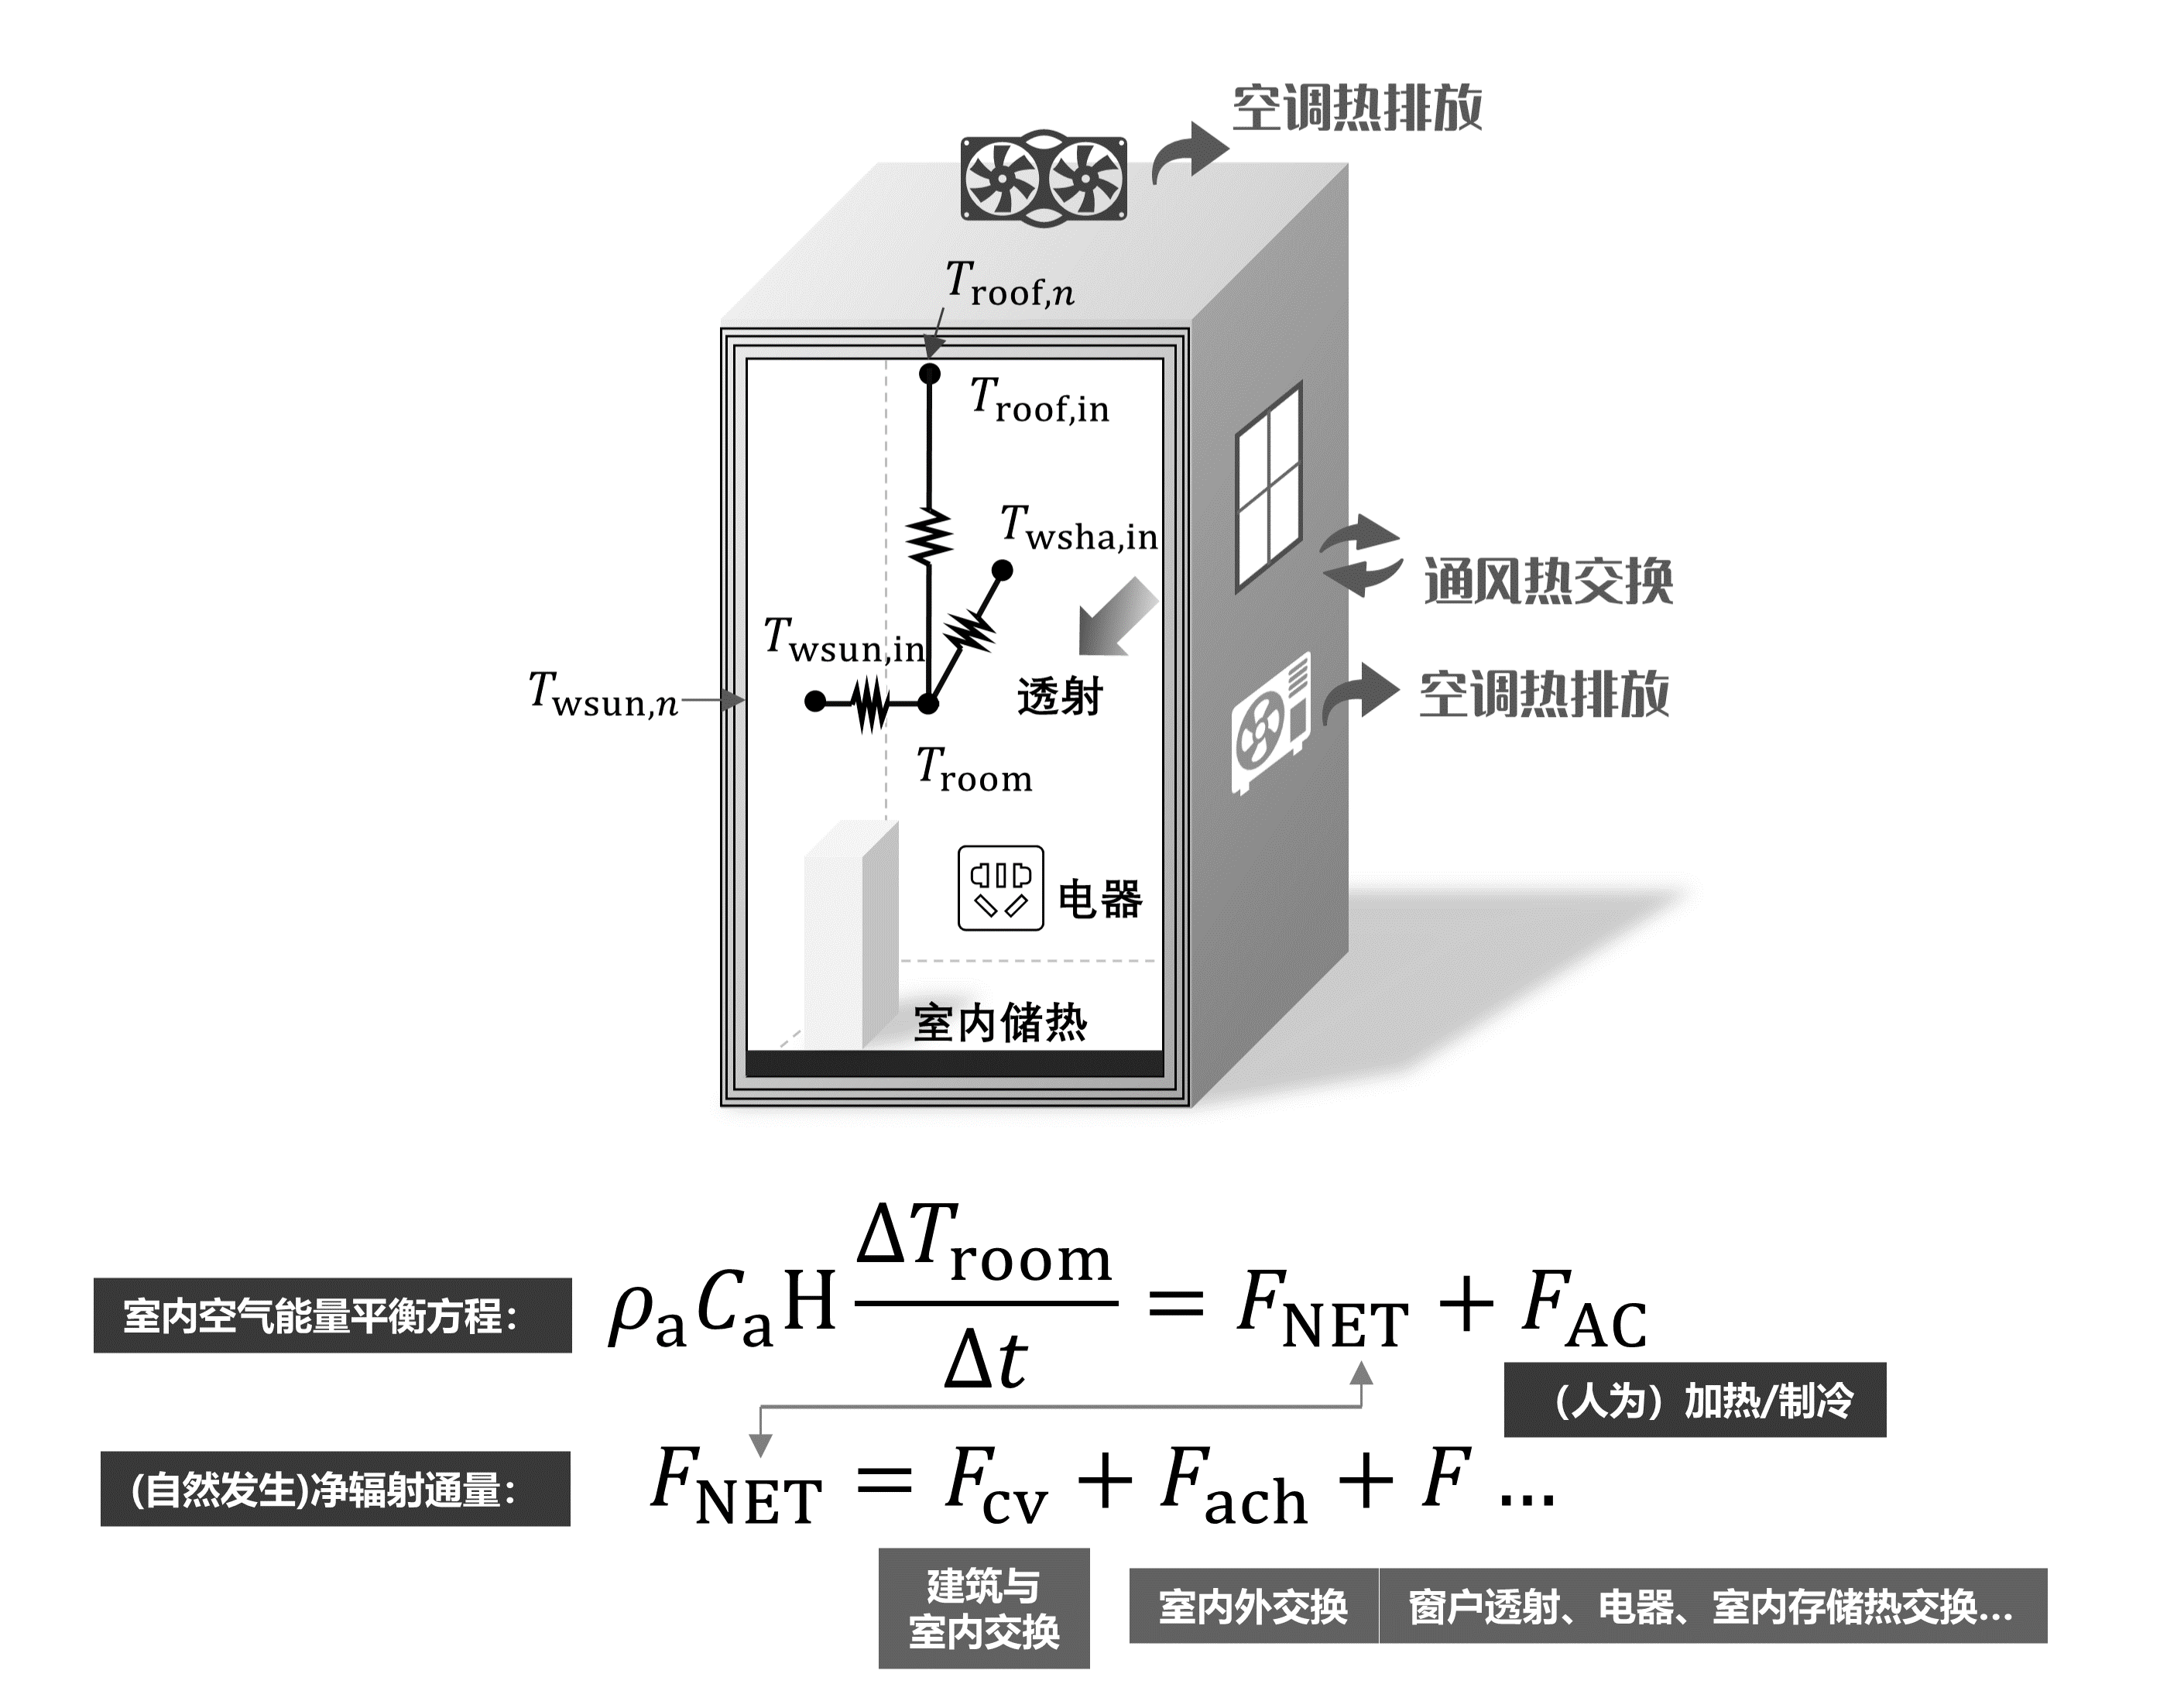
\includegraphics[width=0.75\textwidth]{Figures/城市模式/CoLM城市模式建筑能耗示意图_v2.png}
    \caption[CoLM城市模式建筑能耗模型示意图]{CoLM城市模式建筑能耗模型示意图。图中所示由窗户透射、电器及室内储热带来的热交换依赖于建筑属性,在已知相关参数的前提下可以加入到能耗模型平衡方程中进行计算}
    \label{fig:建筑能耗模型示意图}
  \end{figure}
}

CoLM建筑物能耗模型如图~\ref{fig:建筑能耗模型示意图} 所示,同样是基于三维城市建筑群落结构假设。
模型考虑墙体、屋顶的热传导过程,同时考虑室内空气与内墙壁、屋顶和室外的热量交换。根据室内设定的最高、最低参考温度,来计算空调对应能耗,以感热的形式增加到湍流交换计算的源项中。也可以部分分配为潜热的形式排放,在已知空调排放形式前提下。

基本思路如下:

\begin{enumerate}
  \item 在不打开空调的情况下,通过室内能量平衡方程预报室内温度;
  \item 如果室内温度在预先设定的舒适度范围内,则不再进一步进行能耗计算,仅计算室内外热量交换;
  \item 如果室内温度在预先设定的舒适度范围外,则根据空调使用策略计算达到的最低/最高温度制热/制冷量;
  \item 根据3所计算的制热/制冷量计算室内外交换热、废热排放(涉及能源利用效率),最后可根据总的热量通量来计算能源消耗。
\end{enumerate}

求解过程首先列出热通量交换表达式,并建立能量平衡方程,进而求解室内温度$T_{\mathrm{room}}$,室内墙壁表面空气温度$T_{\mathrm{wsun,in}}$,$T_{\mathrm{wsha,in}}$和室内屋顶表面空气温度$T_{\mathrm{roof,in}}$。
通量交换包括最里层墙壁/屋顶与屋内墙壁/屋顶表面空气热量交换,屋内墙壁/屋顶表面空气与室内空气热量交换以及室内空气与室外空气热量交换,通量平衡方程为:
\begin{landscape}
  \begin{equation}
    \begin{array}{l}
      \begin{split}
        0.5 h_{\mathrm{cv,{roof }}}\left(t_{\mathrm{{roof }}, { in }}-t_{\mathrm{{room }}}\right)+0.5 h_{\mathrm{cv,{roof }}}\left(t_{\mathrm{{roof,in }}}^{\prime}-t_{\mathrm{{room }}}^{\prime}\right)=0.5 h_{\mathrm{tk,{roof}}}\left(T_{\mathrm{{roof }}, n}-T_{\mathrm{{roof }}, { in }}\right)+0.5 h_{\mathrm{tk,{roof }}}\left(T_{\mathrm{{roof }}, n}-T_{\mathrm{{roof,in }}}^{\prime}\right) \\
        0.5 h_{\mathrm{cv,{wsun}}}\left(t_{\mathrm{{wsun,in }}}-t_{\mathrm{{room }}}\right)+0.5 h_{\mathrm{cv,{wsun}}}\left(t_{\mathrm{wsun, i n}}^{\prime}-t_{\mathrm{{room }}}^{\prime}\right)=0.5 h_{\mathrm{tk,{wsun}}}\left(T_{\mathrm{{wsun, }} n}-T_{\mathrm{{wsun,in }}}\right)+0.5 h_{\mathrm{tk,{roof}}}\left(T_{\mathrm{{wsun, }} n}-T_{\mathrm{{wsun,in }}}^{\prime}\right)\\
        0.5 h_{\mathrm{cv,wsha}}\left(t_{\mathrm{wsha, i n}}-t_{\mathrm{{room }}}\right)+0.5 h_{\mathrm{cv,wsha}}\left(t_{\mathrm{wsha, i n}}^{\prime}-t_{\mathrm{{room }}}^{\prime}\right)=0.5 h_{\mathrm{tk,wsha}}\left(T_{\mathrm{wsha, n}}-T_{\mathrm{{roof }}, i n}\right)+0.5 h_{\mathrm{tk,wsha}}\left(T_{\mathrm{wsha, n}}-T_{\mathrm{wsha, i n}}^{\prime}\right)\\
        H \rho_{\mathrm{a}} C_{\mathrm{a}} \frac{T_{\mathrm{{room }}}^{\prime}-T_{\mathrm{{room }}}}{\Delta t}
        =\frac{\mathrm {ACH}}{3600} H \rho_{\mathrm{a}} C_{\mathrm{a}}\left(T_{\mathrm{a f}}-T_{\mathrm{{room }}}^{\prime}\right)+0.5 h_{\mathrm{cv,{roof}}}\left(t_{\mathrm{{roof }}, { in }}-t_{\mathrm{{room }}}\right)+0.5 h_{\mathrm{cv,{roof }}}\left(t_{\mathrm{{roof }}, { in }}^{\prime}-t_{\mathrm{{room }}}^{\prime}\right)\\
        +0.5 h_{\mathrm{cv,wsun}}\left(t_{\mathrm{wsun, i n}}-t_{\mathrm{{room }}}\right) f_{\mathrm{{wsun }}}+0.5 h_{\mathrm{cv,wsun}}\left(t_{\mathrm{wsun, i n}}^{\prime}-t_{\mathrm{{room }}}^{\prime}\right) f_{\mathrm{wsun}} \\
        +0.5 h_{\mathrm{cv,wsha}}\left(t_{\mathrm{wsha, i n}}-t_{\mathrm{{room }}}\right) f_{\mathrm{wsha}}+0.5 h_{\mathrm{cv,wsha}}\left(t_{\mathrm{wsha, i n}}^{\prime}-t_{\mathrm{r o o m}}^{\prime}\right) f_{\mathrm{wsha}}
      \end{split}
    \end{array}
  \end{equation}
  \vspace{-5pt}
  以上方程组可写成矩阵形式:
  \vspace{-5pt}
  \begin{equation}\label{eq:建筑能耗平衡方程矩阵}
    \begin{split}
      \left(\begin{array}{cccc}0.5 h_{\mathrm{cv,roof}}+0.5 h_{\mathrm{tk,roof}} & 0 & 0 & -0.5 h_{\mathrm{cv,roof}} \\ 0 & 0.5 h_{\mathrm{cv,wsun}}+0.5 h_{\mathrm{tk,wsun}} & 0 & -0.5 h_{\mathrm{cv,wsun}} \\ 0 & 0 & 0.5 h_{\mathrm{cv,wsha}}+0.5 h_{\mathrm{tk,wsha}} & -0.5 h_{\mathrm{cv,wsha}} \\ -0.5 h_{\mathrm{cv,roof}} & -0.5 h_{\mathrm{cv,wsun}} f_{\mathrm{wsun}} & -0.5 h_{\mathrm{cv,wsha}} f_{\mathrm{wsha}} & \xi + \frac{H \rho_{\mathrm{a}} C_{\mathrm{a}}}{\Delta t}+\frac{{ \mathrm {ACH} }}{3600} H \rho_{\mathrm{a}} C_{\mathrm{a}}\end{array}\right)
      \left(\begin{array}{c}T_{\mathrm{{roof,in }}}^{\prime} \\ T_{\mathrm{wsun, i n}}^{\prime} \\ T_{\mathrm{wsha, i n}}^{\prime} \\ T_{\mathrm{{room }}}^{\prime}\end{array}\right)=
      \\
      \left(\begin{array}{c}-0.5h_{\mathrm{cv,roof}}\left(t_{\mathrm{roof,in}}-t_{\mathrm{room}}\right)+0.5h_{\mathrm{tk,roof}}\left(T_{\mathrm{roof,n}}-T_{\mathrm{roof,in}}\right)+0.5h_{\mathrm{tk,roof}}T_{\mathrm{roof,n}}\\
          -0.5h_{\mathrm{cv,wsun}}\left(t_{\mathrm{wsun,in}}-t_{\mathrm{room}}\right)+0.5h_{\mathrm{tk,wsun}}\left(T_{\mathrm{wsun,n}}-T_{\mathrm{wsun,in}}\right)+0.5h_{\mathrm{tk,wsun}}T_{\mathrm{wsun,n}}\\
          -0.5h_{\mathrm{cv,wsha}}\left(t_{\mathrm{wsha,in}}-t_{\mathrm{room}}\right)+0.5h_{\mathrm{tk,wsun}}\left(T_{\mathrm{wsun,n}}-T_{\mathrm{wsun,in}}\right)+0.5h_{\mathrm{tk,wsha}}T_{\mathrm{wsun,n}}\\
          \frac{H \rho_{\mathrm{a}} C_{\mathrm{a}} T_{\mathrm{{room }}}}{\Delta T}+\frac{\mathrm {ACH}}{3600} H \rho_{\mathrm{a}} C_{\mathrm{a}} T_{\mathrm{a f}}+0.5 h_{\mathrm{{cv,roof}}}\left(t_{\mathrm{{roof,in }}}-t_{\mathrm{{room }}}\right)+0.5 h_{\mathrm{{cv,wsun}}}\left(t_{\mathrm{{wsun,in }}}-t_{\mathrm{{room }}}\right) f_{\mathrm{{wsun }}}+0.5 h_{\mathrm{{cv,wsha}}}\left(t_{\mathrm{wsha, i n}}-t_{\mathrm{{room }}}\right) f_{\mathrm{{wsha }}}
      \end{array}\right)
    \end{split}
  \end{equation}
  注:上式中$\xi = 0.5 h_{\mathrm{cv,roof}} + 0.5 h_{\mathrm{cv,wsun}}f_{\mathrm{wsun}} + 0.5 h_{\mathrm{cv,wsha}} f_{\mathrm{wsha}} $。
\end{landscape}
\noindent 上式可简写为以下矩阵形式:
\begin{equation}
  \mathbf{Ax}=\mathbf{B}
\end{equation}
公式~\eqref{eq:建筑能耗平衡方程矩阵} 中$T_{\mathrm{roof,in}}^\prime$、$T_{\mathrm{wsun,in}}^\prime$、$T_{\mathrm{wsha,in}}^\prime$、$T_{\mathrm{room}}^\prime$为需求解(预报)变量,其他变量均为已知量。
$T_{\mathrm{roof,in}}$、$T_{\mathrm{wsun,in}}$、$T_{\mathrm{wsha,in}}$、$T_{\mathrm{room}}$分别为上一时刻相应温度,$T_{\mathrm{af}}$为建筑室外空气温度。
$h_{\mathrm{cv,roof}}$、$h_{\mathrm{cv,wsun}}$、$h_{\mathrm{cv,wsha}}$分别为室内屋顶表面空气、阳面、阴面墙表面空气与室内空气温度热交换系数,参考CLM5.0~\citep{oleson2020parameterization},$h_{\mathrm{cv,roof}}=4.04$,$h_{\mathrm{cv,wsun}}=h_{\mathrm{cv,wsha}}=3.076$。$\mathrm {ACH}$为室内外空气热交换系数,设置为0.3。
$T_{\mathrm{roof}}$、$T_{\mathrm{wsun,n}}$、$T_{\mathrm{wsha,n}}$为最里层(用$n$表示)
屋顶、阴面墙、阳面墙的温度,为$h_{\mathrm{tk,roof}}$、$h_{\mathrm{tk,wsun}}$、$h_{\mathrm{tk,wsha}}$为其与各自室内表面空气温度热交换系数,通过墙壁导热率和厚度计算得到。
以上方程组可通过矩阵求逆的方式进行求解,计算得到$T_{\mathrm{roof,in}}^\prime$、$T_{\mathrm{wsun,in}}^\prime$、$T_{\mathrm{wsha,in}}^\prime$、$T_{\mathrm{room}}^\prime$。

当$T_{\mathrm{room,min}}\leqslant T_{\mathrm{room}}^\prime \leqslant T_{\mathrm{room,max}} $ ($T_{\mathrm{room,min}}$和$T_{\mathrm{room,max}}$为预设屋内最低/最高温度,从外部数据读取)时,室内空调不开启,仅考虑室内外热交换通量$F_{\mathrm{ach}}$,计算为:
\begin{equation}
  F_{\mathrm{a c h}}=\frac{\mathrm {ACH}}{3600} H \rho_{\mathrm{a}} C_{\mathrm{a}}\left(T_{\mathrm{{room }}}^{\prime}-T_{\mathrm{a f}}\right)
\end{equation}

当$T_{\mathrm{room}}^\prime>T_{\mathrm{room,max}}$或者$T_{\mathrm{room}}^\prime<T_{\mathrm{room,min}}$时,需要打开空调进行制冷或制热。目前CoLM提供两种空调使用策略:1) 按需制冷/制热;2) 持续制冷/制热。分别描述如下:

\textit{1) 按需制冷/制热}

当$T_{\mathrm{room}}^\prime>T_{\mathrm{room,max}}$时,需打开空调制冷,制冷量为使屋内温度下降到$T_{\mathrm{room,max}}$,由此所需要的空调制冷量$F_{\mathrm{hac}}$计算为:
\begin{equation}
  F_{\mathrm{{hac }}}=H \rho_{\mathrm{a}} C_{\mathrm{a}} \frac{T_{\mathrm{{room }}}^{\prime}-T_{\mathrm{{room,max }}}}{\Delta t}
\end{equation}

当$T_{\mathrm{room}}^\prime<T_{\mathrm{room,min}}$时,需打开制暖设备,制热量为使屋内温度上升到$T_{\mathrm{room,min}}$,由此产生的空调热制热量$F_{\mathrm{hac}}$计算为:
\begin{equation}
  F_{\mathrm{h a c}}=H \rho_{\mathrm{a}} C_{\mathrm{a}} \frac{T_{\mathrm{{room,min }}} -T_{\mathrm{{room }}}^{\prime}}{\Delta t}
\end{equation}
在以上两种情况下,$T_{\mathrm{room}}^\prime$最终更新为$T_{\mathrm{room,max}}/T_{\mathrm{room,min}}$。
由于制冷/制暖所浪费的热量排放分别计算为$0.6F_{\mathrm{hac}}$和$0.2F_{\mathrm{hac}}$。

\textit{2) 持续制冷/制热}

按需制冷方案是一种比较理想的空调使用策略,最大程度节约能源,但实际中一般难以实现,更多的空调使用情况是持续制冷/制热,来维持室内空气温度到固定值。因此,本方案较方案(1)会更消耗能源。

当$T_{\mathrm{room}}^\prime>T_{\mathrm{room,max}}$或$T_{\mathrm{room}}^\prime<T_{\mathrm{room,min}}$时,设置室内空气温度恒定为$T_{\mathrm{room,max}}$ \allowbreak($T_{\mathrm{room,min}}$),室内外热交换通量$F_{\mathrm{ach}}$计算为:
\begin{equation}
  F_{\mathrm{a c h}}=\frac{\mathrm {ACH}}{3600} H \rho_{\mathrm{a}} C_{\mathrm{a}}\left(T_{\mathrm{{room,max/min}}}-T_{\mathrm{a f}}\right)
\end{equation}

由于$T_{\mathrm{room}}^\prime$维持在恒定温度,因此$T_{\mathrm{roof,in}}^\prime$、$T_{\mathrm{wsun,in}}^\prime$、$T_{\mathrm{wsha,in}}^\prime$需重新进行计算,根据热通量平衡方程可得:
\begin{equation}
  \begin{aligned}
    T_{\mathrm{roof,in}}^\prime & = \left ( \mathbf{B}\left(1\right)-\mathbf{A}\left(1,4\right)T_{\mathrm{room}}^\prime\right) / \mathbf{A}\left(1,1\right) \\
    T_{\mathrm{wsun,in}}^\prime & = \left ( \mathbf{B}\left(2\right)-\mathbf{A}\left(2,4\right)T_{\mathrm{room}}^\prime\right) / \mathbf{A}\left(2,2\right) \\
    T_{\mathrm{wsha,in}}^\prime & = \left ( \mathbf{B}\left(3\right)-\mathbf{A}\left(3,4\right)T_{\mathrm{room}}^\prime\right) / \mathbf{A}\left(3,3\right)
  \end{aligned}
\end{equation}
空调制冷/热制热量$F_{\mathrm{hac}}$计算为:
\begin{equation}
  \begin{aligned}
    F_{\mathrm{ach}} & = 0.5h_{\mathrm{cv,roof}}\left(T_{\mathrm{roof,in}}-T_{\mathrm{room}}\right) + 0.5h_{\mathrm{cv,roof}}\left(T_{\mathrm{roof,in}}^\prime-T_{\mathrm{room}}^\prime\right) \\
    & + 0.5h_{\mathrm{cv,wsun}}\left(T_{\mathrm{wsun,in}}-T_{\mathrm{room}}\right)f_{\mathrm{wsun}} + 0.5h_{\mathrm{cv,wsun}}\left(T_{\mathrm{wsun,in}}^\prime-T_{\mathrm{room}}^\prime\right)f_{\mathrm{wsun}} \\
    & + 0.5h_{\mathrm{cv,wsha}}\left(T_{\mathrm{wsha,in}}-T_{\mathrm{room}}\right)f_{\mathrm{wsha}} + 0.5h_{\mathrm{cv,wsha}}\left(T_{\mathrm{wsha,in}}^\prime-T_{\mathrm{room}}^\prime\right)f_{\mathrm{wsha}}
  \end{aligned}
\end{equation}
由于制冷/制暖所浪费的热排放$F_{\mathrm{wst}}$分别计算为$0.6\left( |F_{\mathrm{hac}}|+|F_{\mathrm{ach}}|\right)$和$0.2\left( |F_{\mathrm{hac}}|+|F_{\mathrm{ach}}|\right)$,| |表示取绝对值。

总的建筑热排放量为制冷/制暖热排放量加上其过程中浪费的热排放量。需要注意,制冷时,$F_{\mathrm{hac}}+F_{\mathrm{wst}}$作为人为热在室外排放;制热时,仅$F_{\mathrm{wst}}$作为室外人为热排放,此时$F_{\mathrm{hac}}$作为室内空气加热。以上计算的热通量均需乘以$f_{\rm b}$来转化为单位城市面积通量,
$F_{\mathrm{hac}}, F_{\mathrm{wst}}$和$F_{\mathrm{ach}}$作为感热项 (源项) 加入到城市湍流交换平衡方程中,参考图~\ref{fig:建筑能耗模型示意图}。

\subsection{交通热}
\esubsection{Traffic Heat}
\begin{mymdframed}{代码}
  本节及下节对应的代码文件为\texttt{MOD\_Urban\_LUCY.F90}。
\end{mymdframed}

交通热排放($Q_{\rm v}$, \unit{W.m^{-2}})则根据城市网格内的汽车数量以及行驶路程得到,首先根据城市网格内的人口密度以及各个地区每千人汽车拥有量计算出格点内的汽车数量,然后根据汽车行驶排放的热量以及交通流量的日分布计算出不同时刻的交通热排放。
其数据来源如表~\ref{tab:交通热数据及来源},$Q_{\rm v}$计算如下:
\begin{equation}
  Q_{\mathrm{v}}=\frac{\left(V_{\mathrm{c}} E_{\mathrm{c}}+V_{\mathrm{M}} E_{\mathrm{M}}+V_{\mathrm{F R}} E_{\mathrm{FR}}\right)  \cdot P \cdot H_{\mathrm{traf}} \cdot D}{3600 \cdot 10^{6}}
\end{equation}
其中$V_{\mathrm {c}}$、$V_{\mathrm {M}}$、$V_{\mathrm{FR}}$分别为每千人拥有的汽车、摩托车、货车(巴士)的数量,$H_{\mathrm{traf}}$为工作日/休息日某一时间段交通流量,以上数据来源于 \citet{allen2011};$E_{\mathrm {c}}$、$E_{\mathrm {M}}$、$E_{\mathrm{FR}}$则为三种机动车的排放系数,目前使用 \citet{sailor2004top} 的参数设置(\qty{3975}{J.m^{-1}});
$P$为格点内人口密度 (\unit{pop.km^{-2}}),由LandScan数据得到;$D$为行驶的距离,目前模型设置为50 km。

\begin{table}[htbp]
  \centering
  \caption{交通热数据及来源}\label{tab:交通热数据及来源}
  \begin{tabular}{@{}lll@{}}
    \toprule
    数据名称                   & 来源                   & Spatial/administrative unit   \\ \midrule
    Vehicles density and types & World mapper           & All countries and territories \\
    Daily vehicle pattern      & \citet{Hallenbeck1997} & All countries and territories \\ \bottomrule
  \end{tabular}
\end{table}

\subsection{人体代谢热}
\esubsection{Human Metabolic Heat}

\begin{mymdframed}{代码}
  本节及下节对应的代码文件为\texttt{MOD\_Urban\_LUCY.F90}。
\end{mymdframed}

人体代谢热($Q_{\mathrm {M}}$, \unit{W.m^{-2}})根据 \citet{allen2011} 的方法,根据城市网格内的人口密度数据,以及每天不同时刻的人体热排放计算得到,具体计算如下:
%
\begin{equation}
  Q_{\mathrm{M}}=P \cdot H_{\mathrm{M}} \cdot 10^{-6}
\end{equation}
%
其中$P$为格点内人口密度(\unit{pop.km^{-2}}),目前使用的是 LandScan 数据(表~\ref{tab:人口密度数据}),分辨率为1 km,$H_{\mathrm M}$为不同时刻人体排放的热量。人体排放的热量采用简单假设:
人在活动时每小时排放的热量为175 W (工作),非活动时排放量为75 W (休息),以及一个中间值125 W~\citep{sailor2004top}。
除此之外,没有考虑人口在不同格点间的移动。
%
\begin{table}[htbp]
  \centering
  \caption{人口密度数据}
  \label{tab:人口密度数据}
  \begin{tabular}{@{}lll@{}}
    \toprule
    数据名称 & 分辨率 & 来源                                                                     \\ \midrule
    LandScan & 1km    & \begin{tabular}[c]{@{}l@{}}\url{https://landscan.ornl.gov/}\end{tabular} \\ \bottomrule
  \end{tabular}
\end{table}

\subsection{考虑人为热时城市内部湍流交换}
\esubsection{Urban Turbulent Exchange with Anthropogenic Heat}

\begin{mymdframed}{代码}
  本节及下节对应的代码文件为\texttt{MOD\_Urban\_Flux.F90}。
\end{mymdframed}
{
  \begin{figure}[h!]
    \centering
    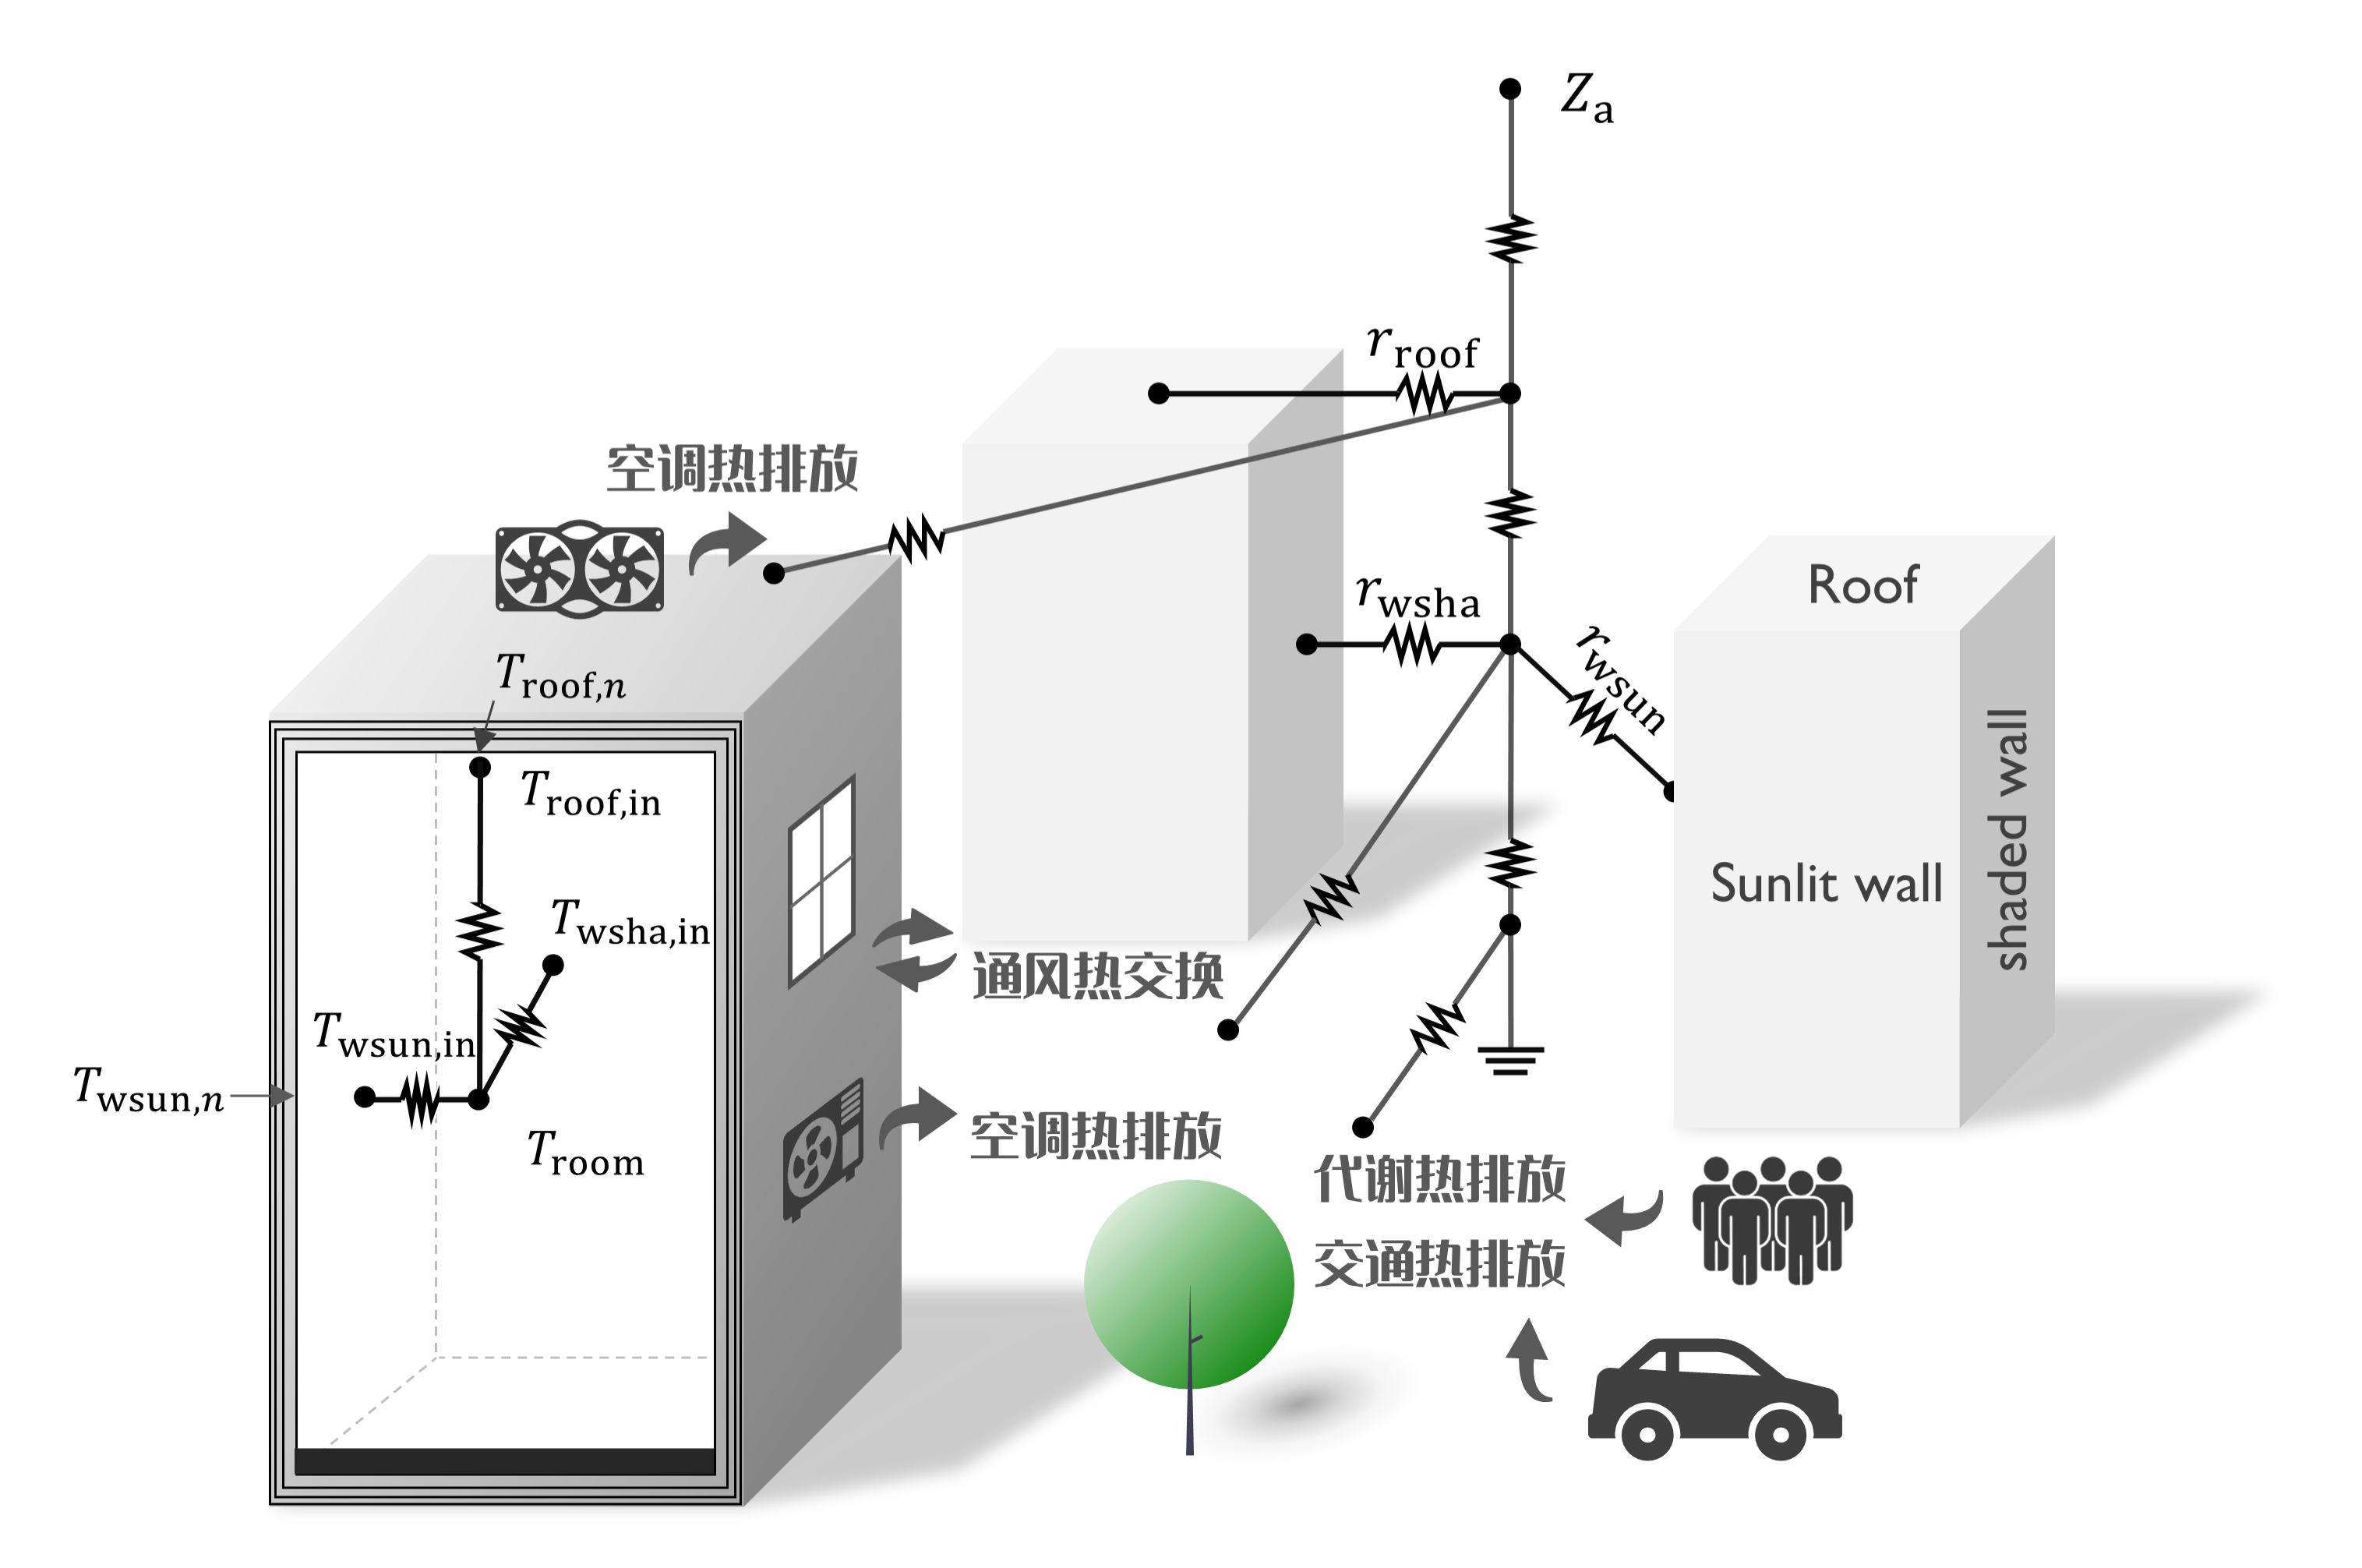
\includegraphics[width=0.75\textwidth]{Figures/城市模式/CoLM城市模式人为热阻抗交换网络_v2.png}
    \caption{考虑人为热时城市湍流交换阻抗网络示意图}
    \label{fig:考虑人为热时城市内部湍流交换过程}
  \end{figure}
}
\subsubsection{两层交换方案}\label{人为热两层方案}
考虑人为热时,城市内部湍流过程示意图~\ref{fig:考虑人为热时城市内部湍流交换过程} 所示,与章节~\ref{城市湍流过程} 相同,在建筑群落中,不同的城市组成部分在不同层次进行交换。以两层交换阻抗网络为例(植被高度与建筑高度相近时),与第二层(建筑墙面等效交换高度$z_0+d$)直接交换的有地面(透水面与不透水面)、墙面(阳面墙与阴面墙)、植被、交通热、代谢热以及部分在墙面排放的人为热,屋顶与屋顶释放的人为热则与第三层(即屋顶)直接交换,层与层交换保持通量平衡。因此,对于感热而言,其不同层次的感热通量$H$可表达为:
\begin{equation}\label{2lays_H_layer2}
  H_{\mathrm{2}} = H_{\mathrm{g}}
\end{equation}
%
\begin{equation}\label{2lays_H_layer3}
  H_{3} = H_{2} + H_{\mathrm{wsun}} + H_{\mathrm{wsha}} + H_{\mathrm{v}} + H_{\mathrm{whac}} = \frac{\rho _{\rm a} C_{\mathrm a} \left( T_{2} - T_{3} \right)}{r_{\mathrm{d3}}}
\end{equation}
%
\begin{equation}\label{2lays_H}
  H = H_{3} + H_{\mathrm{roof}} + H_{\mathrm{rhac}} = \frac{\rho _{\rm a} C_{\mathrm a} \left( T_{3} - T_{\rm a} \right)}{r_{\mathrm{ah}}}
\end{equation}
其中,$H_2$、$H_3$以及$H$同样为地面与第二层、第二层与第三层以及第三层与参考高度的感热通量交换,$H_{\mathrm{whac}}$、$H_{\mathrm{rhac}}$为墙面以及屋顶释放的建筑热,根据建筑能耗模型计算得到(章节~\ref{建筑能耗模型}),$H_{\mathrm{g}}$、$H_{\mathrm{wsun}}$、$H_{\mathrm{wsha}}$、$H_{\mathrm{v}}$、$H_{\mathrm{roof}}$分别为地面、阳面墙、阴面墙、植被以及屋顶的感热通量,其各自的表达式分别为:
\begin{equation}\label{urban_Hg}
  H_{\mathrm{g}} = \frac{\rho _{\rm a} C_{\mathrm a} \left( T_{\mathrm{g}} - T_{2} \right) \cdot f_{\mathrm{g}}}{r_{\mathrm{d2}}} + H_{\mathrm{vehc}} + H_{\mathrm{meta}}
\end{equation}
%
\begin{equation}
  H_{\mathrm{wsun}} = \frac{\rho  _{\rm a} C_{\mathrm a} \left( T_{\mathrm{wsun}} - T_{\mathrm{2}} \right) \cdot f_{\mathrm{wsun}}}{r_{\mathrm{wsun}}}
\end{equation}
%
\begin{equation}
  H_{\mathrm{wsha}} = \frac{\rho _{\rm a} C_{\mathrm a} \left( T_{\mathrm{wsha}} - T_{\mathrm{2}} \right) \cdot f_{\mathrm{wsha}}}{r_{\mathrm{wsha}}}
\end{equation}
%
\begin{equation}
  H_{\mathrm{v}} = \frac{\rho _{\rm a} C_{\mathrm a} \left( T_{\mathrm{v}} - T_{2} \right) \cdot f_{\rm v}}{r_{\mathrm{v}}}
\end{equation}
%
\begin{equation}\label{urban_Hroof}
  H_{\mathrm{roof}} = \frac{\rho _{\rm a} C_{\mathrm a} \left( T_{\mathrm{roof}} - T_{3} \right) \cdot f_{\mathrm{roof}}}{r_{\mathrm{roof}}}
\end{equation}
$T_2$和$T_3$分别表示第二层和第三层空气温度。由于代谢热与交通热($H_{\mathrm{meta}}$ 、$H_{\mathrm{vehc}}$)都在地面释放,因此我们将其纳入地面感热$H_{\mathrm{g}}$。其中$T_{\mathrm{g}}$为透水面与不透水面温度加权得到的平均温度,$r$为空气动力学阻抗,\allowbreak $f_{\mathrm{roof}}$、\allowbreak $f_{\mathrm{wsun}}$、\allowbreak $f_{\mathrm{wsha}}$、\allowbreak $f_{\rm v}$分别代表屋顶、阳面墙、阴面墙以及植被的覆盖比例,$f_{\mathrm{g}}$则为除去建筑覆盖外的路面占比(包含透水面$f_{\mathrm{gper}}$以及不透水面$f_{\mathrm{gimp}}$),将以上表达式代回公式~\eqref{2lays_H_layer2}--\eqref{2lays_H},可得:
\begin{equation}
  \begin{split}
    & \frac{\rho _{\rm a} C_{\mathrm a} \left( T_{2} - T_{3} \right)}{r_{\mathrm{d3}}} = \\
    & \frac{\rho _{\rm a} C_{\mathrm a} \left( T_{\mathrm{g}} - T_{2} \right) \cdot f_{\mathrm{g}}}{r_{\mathrm{d2}}} + \frac{\rho _{\rm a} C_{\mathrm a} \left( T_{\mathrm{wsun}} - T_{2} \right) \cdot f_{\mathrm{wsun}}}{r_{\mathrm{wsun}}} + \frac{\rho _{\rm a} C_{\mathrm a} \left( T_{\mathrm{wsha}} - T_{2} \right) \cdot f_{\mathrm{wsha}}}{r_{\mathrm{wsha}}} +
    \\
    & \frac{\rho _{\rm a} C_{\mathrm a} \left( T_{\mathrm{v}} - T_{2} \right) \cdot f_{\rm v}}{r_{\mathrm{v}}} + H_{\mathrm{AHE3}}
        % + H_{\mathrm{whac}} + H_{\mathrm{vehc}} + H_{\mathrm{meta}}
  \end{split}
\end{equation}
%
\begin{equation}
  \begin{split}
    \frac{\rho _{\rm a} C_{\mathrm a} \left( T_{3} - T_{\rm a} \right)}{r_{\mathrm{ah}}} =
    \frac{\rho _{\rm a} C_{\mathrm a} \left( T_{2} - T_{3} \right)}{r_{\mathrm{d3}}} + \frac{\rho _{\rm a} C_{\mathrm a} \left( T_{\mathrm{roof}} - T_{3} \right)\cdot f_{\mathrm{roof}}}{r_{\mathrm{roof}}} + H_{\mathrm{AHE3}}
  \end{split}
\end{equation}
其中:
\begin{equation}
  H_{\mathrm{AHE2}} = H_{\mathrm{whac}} + H_{\mathrm{vehc}} + H_{\mathrm{meta}}
\end{equation}
%
\begin{equation}
  H_{\mathrm{AHE3}} = H_{\mathrm{rhac}}
\end{equation}
进而得到关于$T_{2}$和$T_{3}$的二元一次方程:
\begin{equation}
  \begin{split}
    T_{2} =
    \frac{\frac{T_{\mathrm{g}} \cdot f_{\mathrm{g}}}{r_{\mathrm{d2}}} + \frac{H_{\mathrm{AHE2}}}{\rho _{\rm a} C_{\mathrm a}} + \frac{T_{\mathrm{wsun}} \cdot f_{\mathrm{wsun}}}{r_{\mathrm{wsun}}} + \frac{T_{\mathrm{wsha}} \cdot f_{\mathrm{wsha}}}{r_{\mathrm{wsha}}} + \frac{T_{\mathrm{v}} \cdot f_{\rm v}}{r_{\mathrm{v}}} + \frac{T_{3}}{r_{\mathrm{d3}}}}{\frac{1}{r_{\mathrm{d3}}} + \frac{f_{\mathrm{g}}}{r_{\mathrm{d2}}} + \frac{f_{\mathrm{wsun}}}{r_{\mathrm{wsun}}} + \frac{f_{\mathrm{wsha}}}{r_{\mathrm{wsha}}} + \frac{f_{\rm v}}{r_{\mathrm{v}}}}
  \end{split}
\end{equation}
%
\begin{equation}\label{result_T_layer3}
  T_{3} = \frac{\frac{T_{2}}{r_{\mathrm{d3}}} + \frac{T_{\mathrm{roof}} \cdot f_{\mathrm{roof}}}{r_{\mathrm{roof}}} + \frac{H_{\mathrm{AHE3}}}{\rho _{\rm a} C_{\mathrm a}} + \frac{T_{\rm a}}{r_{\mathrm{ah}}}}{\frac{1}{r_{\mathrm{ah}}} + \frac{1}{r_{\mathrm{d3}}} + \frac{f_{\mathrm{roof}}}{r_{\mathrm{roof}}}}
\end{equation}
求解该二元一次方程可得:
\begin{equation}
  \begin{split}
    % \hspace{-1cm}
    T_{2} =
    \frac{\frac{T_{\mathrm{g}} \cdot f_{\mathrm{g}}}{r_{\mathrm{d2}}} + \frac{H_{\mathrm{AHE2}}}{\rho _{\rm a} C_{\mathrm a}} + \frac{T_{\mathrm{wsun}} \cdot f_{\mathrm{wsun}}}{r_{\mathrm{wsun}}} + \frac{T_{\mathrm{wsha}} \cdot f_{\mathrm{wsha}}}{r_{\mathrm{wsha}}} + \frac{T_{\mathrm{v}} \cdot f_{\mathrm{v}}}{r_{\mathrm{v}}} + a_{\mathrm{T}}}{c_{\mathrm{T}} \cdot \left( 1 - \frac{b_{\mathrm {T}} }{c_{\mathrm{T}} r_{\mathrm{d3}}} \right)}
  \end{split}
\end{equation}
%
其中:
\begin{equation}
  a_{\mathrm{T}} = \left(\frac{T_{\mathrm{roof}} \cdot f_{\mathrm{roof}}}{r_{\mathrm{roof}}} + \frac{H_{\mathrm{AHE3}}}{\rho _{\rm a} C_{\mathrm a}} + \frac{T_{\rm a}}{r_{\mathrm{ah}}}\right) \cdot b_{\mathrm{T}}
\end{equation}
%
\begin{equation}
  b_{\mathrm{T}} = \frac{1}{r_{\mathrm{d3}} \cdot \left(\frac{1}{r_{\mathrm{ah}}} + \frac{1}{r_{\mathrm{d3}}} + \frac{f_{\mathrm{roof}}}{r_{\mathrm{roof}}} \right)}
\end{equation}
%
\begin{equation}
  c_{\mathrm{T}} = \frac{1}{r_{\mathrm{d3}}} + \frac{f_{\mathrm{g}}}{r_{\mathrm{d2}}} + \frac{f_{\mathrm{wsun}}}{r_{\mathrm{wsun}}} + \frac{f_{\mathrm{wsha}}}{r_{\mathrm{wsha}}} + \frac{f_{\rm v}}{r_{\mathrm{v}}}
\end{equation}
将$T_{2}$代回公式~\eqref{result_T_layer3},即可求得$T_{3}$。

将求解得到的$T_{2}$与$T_{3}$分别代回公式~\eqref{urban_Hg}--\eqref{urban_Hroof},即可得到城市每个表面的感热通量,其后计算城市各表面温度并基于该温度变化对感热通量进行更新时,需要提供各表面感热对各自温度的变化率,各表面分别计算为:
\begin{equation}
  \frac{\partial H_{\mathrm{g}}}{\partial T_{\mathrm{g}}} = \frac{\rho _{\rm a} C_{\mathrm a}}{r_{\mathrm{d2}}} \left(1-\frac{f_{\rm g}}{c_{\mathrm{T}} r_{\mathrm{d2}} \left(1-\frac{b_{\mathrm {T}} }{c_{\mathrm{T}} r_{\mathrm{d3}}}\right)}\right)
\end{equation}
%
\begin{equation}
  \frac{\partial H_{\mathrm{wsun}}}{\partial T_{\mathrm{wsun}}} = \frac{\rho _{\rm a} C_{\mathrm a}}{r_{\mathrm{wsun}}} \left(1-\frac{f_{\mathrm{wsun}}}{c_{\mathrm{T}} r_{\mathrm{wsun}} \left(1-\frac{b_{\mathrm {T}} }{c_{\mathrm{T}} r_{\mathrm{d3}}}\right)}\right)
\end{equation}
%
\begin{equation}
  \frac{\partial H_{\mathrm{wsha}}}{\partial T_{\mathrm{wsha}}} = \frac{\rho _{\rm a} C_{\mathrm a}}{r_{\mathrm{wsha}}} \left(1-\frac{f_{\mathrm{wsha}}}{c_{\mathrm{T}} r_{\mathrm{wsha}} \left(1-\frac{b_{\mathrm {T}} }{c_{\mathrm{T}} r_{\mathrm{d3}}}\right)}\right)
\end{equation}
%
\begin{equation}
  \frac{\partial H_{\mathrm{v}}}{\partial T_{\mathrm{v}}} = \frac{\rho _{\rm a} C_{\mathrm a}}{r_{\mathrm{v}}} \left(1-\frac{f_{\mathrm{v}}}{c_{\mathrm{T}} r_{\mathrm{v}} \left(1-\frac{b_{\mathrm {T}} }{c_{\mathrm{T}} r_{\mathrm{d3}}}\right)}\right)
\end{equation}
%
\begin{equation}
  \frac{\partial H_{\mathrm{roof}}}{\partial T_{\mathrm{roof}}} = \frac{\rho _{\rm a} C_{\mathrm a}}{r_{\mathrm{roof}}} \left(1-\frac{f_{\mathrm{roof}} b_{\mathrm{T}}^2}{c_{\mathrm{T}} r_{\mathrm{roof}} \left(1-\frac{b_{\mathrm {T}} }{c_{\mathrm{T}} r_{\mathrm{d3}}}\right)}-\frac{f_{\mathrm{roof}}}{r_{\mathrm{roof}}\left(\frac{1}{r_{\mathrm{ah}}}+\frac{1}{r_{\mathrm{d3}}}+\frac{f_{\mathrm{roof}}}{r_{\mathrm{roof}}}\right)}\right)
\end{equation}

对于潜热通量而言,其求解过程与感热通量的计算类似,但是在计算潜热通量时,由于墙体难以表达积水过程,因此认为墙体没有潜热交换,并且人为热目前全部作为感热释放,因此,对于潜热通量而言,在第二层发生交换的仅有地面、植被,并且由于考虑土壤阻抗,透水面与不透水面需要单独计算,在第三层发生交换的仅有屋顶,对于不透水面与屋顶,仅考虑积水部分($f_{\mathrm{wet}}$),所以对于建筑群落内部不同层次的潜热通量计算,其表达式为:
\begin{equation}\label{2lays_L_layer2}
  \lambda E_{\mathrm{2}} = \lambda E_{\mathrm{g}}
\end{equation}
%
\begin{equation}
  \lambda E_{3} = \lambda E_{2} + \lambda E_{\mathrm{v}}
\end{equation}
%
\begin{equation}\label{2lays_L}
  \lambda E = \lambda E_{3} + \lambda E_{\mathrm{roof}}
\end{equation}
其中,$ E_{\mathrm{g}}$、$ E_{\mathrm{v}}$、$ E_{\mathrm{roof}}$分别为地面、植被以及屋顶的水汽通量,其表达式分别为:
\begin{equation}\label{urban_Eg}
  E_{\mathrm{g}} = \frac{\rho _{\rm a} \left( q_{\mathrm{gper}}-q_{2} \right) \cdot f_{\mathrm{g}} \cdot f_{\mathrm{gper}}}{r_{\mathrm{d2}}+r_{\mathrm{ss}}} + \frac{\rho _{\rm a} \left( q_{\mathrm{gimp}}-q_{2} \right) \cdot f_{\mathrm{wet,gimp}} \cdot f_{\mathrm{g}} \cdot f_{\mathrm{gimp}}}{r_{\mathrm{d2}}}
\end{equation}
%
\begin{equation}
  E_{\mathrm{v}} = \frac{\rho _{\rm a} \left( q_{\mathrm{v}}-q_{2}\right) \cdot f_{\rm v}}{r_{\mathrm{v}}}
\end{equation}
%
\begin{equation}\label{urban_Eroof}
  E_{\mathrm{roof}} = \frac{\rho _{\rm a} \left( q_{\mathrm{roof}}-q_{3}\right) \cdot f_{\mathrm{wet,roof}} \cdot f_{\mathrm{roof}}}{r_{\mathrm{roof}}}
\end{equation}
由于城市中的地面可以分为透水面和不透水面,对于透水面,因为其本质是土壤,因此在计算其潜热通量时,考虑土壤阻抗($r_{\mathrm{ss}}$),$f_{\mathrm{wet}}$表示各部分干湿的比例,$q$为不同表面的比湿,$r$为空气动力学阻抗,其中$r_{\rm v}$是叶片边界层阻抗以及气孔阻抗之和,将以上表达式代回公式~\eqref{2lays_L_layer2}--\eqref{2lays_L},可知:
\begin{equation}
  \begin{split}
    & \frac{\rho _{\rm a} \left( q_{2}-q_{3}\right)}{r_{\mathrm{d3}}} = \\
    & \frac{\rho _{\rm a} \left( q_{\mathrm{gper}}-q_{\mathrm{2}}\right) \cdot f_{\mathrm{g}} \cdot f_{\mathrm{gper}}}{r_{\mathrm{d2}}+r_{\mathrm{ss}}} + \frac{\rho _{\rm a} \left( q_{\mathrm{gimp}}-q_{2} \right) \cdot f_{\mathrm{wet,gimp}} \cdot f_{\mathrm{g}} \cdot f_{\mathrm{gimp}}}{r_{\mathrm{d2}}} + \frac{\rho _{\rm a} \left( q_{\mathrm{v}}-q_{2}\right) \cdot f_{\rm v}}{r_{\mathrm{v}}}
  \end{split}
\end{equation}
%
\begin{equation}
  \frac{\rho _{\rm a} \left( q_{3} - q_{\rm a}\right)}{r_{\mathrm{aw}}} = \frac{\rho _{\rm a} \left( q_{2} - q_{3}\right)}{r_{\mathrm{d3}}} + \frac{\rho _{\rm a} \left( q_{\mathrm{roof}}-q_{3}\right) \cdot f_{\mathrm{wet,roof}} \cdot f_{\mathrm{roof}}}{r_{\mathrm{roof}}}
\end{equation}
同样可得关于$q_{2}$以及$q_{3}$的二元一次方程:
\begin{equation}
  q_{2} = \\
  \frac{\frac{q_{\mathrm{gper}} \cdot f_{\mathrm{g}} \cdot f_{\mathrm{gper}}}{r_{\mathrm{d2}} + r_{\mathrm{ss}}} + \frac{q_{\mathrm{gimp}} \cdot f_{\mathrm{wet,gimp}} \cdot f_{\mathrm{g}} \cdot f_{\mathrm{gimp}}}{r_{\mathrm{d2}}} + \frac{q_{\mathrm{v}} \cdot f_{\rm v}}{r_{\mathrm{v}}} + \frac{q_{\mathrm{3}}}{r_{\mathrm{d3}}}}{\frac{1}{r_{\mathrm{d3}}} + \frac{f_{\mathrm{g}} \cdot f_{\mathrm{gper}}}{r_{\mathrm{d2}} + r_{\mathrm{ss}}} + \frac{f_{\mathrm{wet,gimp}} \cdot f_{\mathrm{g}} \cdot f_{\mathrm{gimp}}}{r_{\mathrm{d2}}}+\frac{f_{\rm v}}{r_{\mathrm{v}}}}
\end{equation}
%
\begin{equation}\label{equ_2lays_Q_lay3}
  q_{3} = \frac{\frac{q_{2}}{r_{\mathrm{d3}}} + \frac{q_{\mathrm{roof}} \cdot f_{\mathrm{wet,roof}} \cdot f_{\mathrm{roof}}}{r_{\mathrm{roof}}} + \frac{q_{\rm a}}{r_{\mathrm{aw}}}}{\frac{1}{r_{\mathrm{aw}}} + \frac{1}{r_{\mathrm{d3}}} + \frac{f_{\mathrm{wet,roof}} \cdot f_{\mathrm{roof}}}{r_{\mathrm{roof}}}}
\end{equation}
求解可得:
\begin{equation}
  q_{2} = \\
  \frac{\frac{q_{\mathrm{gper}} \cdot f_{\mathrm{g}} \cdot f_{\mathrm{gper}}}{r_{\mathrm{d2}}+r_{\mathrm{ss}}} + \frac{q_{\mathrm{gimp}} \cdot f_{\mathrm{wet,gimp}} \cdot f_{\mathrm{g}} \cdot f_{\mathrm{gimp}}}{r_{\mathrm{d2}} } + \frac{q_{\mathrm{v}} \cdot f_{\rm v}}{r_{\mathrm{v}}} + a_{\mathrm{q}}}{c_{\mathrm{q}} \cdot \left( 1 - \frac{b_{\mathrm{q}}}{c_{\mathrm{q}} \cdot r_{\mathrm{d3}}}\right)}
\end{equation}
%
其中:
\begin{equation}
  a_{\mathrm{q}}= \left(\frac{q_{\mathrm{roof}} \cdot f_{\mathrm{wet,roof}} \cdot f_{\mathrm{roof}}}{r_{\mathrm{roof}}} + \frac{q_{\rm a}}{r_{\mathrm{aw}}}\right) \cdot b_{\mathrm{q}}
\end{equation}
%
\begin{equation}
  b_{\mathrm{q}} = \frac{1}{r_{\mathrm{d3}} \cdot \left( \frac{1}{r_{\mathrm{aw}}} + \frac{1}{r_{\mathrm{d3}}} + \frac{f_{\mathrm{wet,roof}} \cdot f_{\mathrm{roof}}}{r_{\mathrm{roof}}} \right)}
\end{equation}
%
\begin{equation}
  c_{\mathrm{q}} = \frac{1}{r_{\mathrm{d3}}}+\frac{f_{\rm g} \cdot f_{\mathrm{gper}}}{r_{\mathrm{d3}}+r_{\mathrm{ss}}} + \frac{f_{\mathrm{wet,gimp}} \cdot f_{\rm g} \cdot f_{\mathrm{gimp}}}{r_{\mathrm{d2}}} + \frac{f_{\rm v}}{r_{\mathrm{v}}}
\end{equation}
同理,将$q_{\mathrm{2}}$代入公式~\eqref{equ_2lays_Q_lay3} 即可求得$q_{3}$。

将求解得到的$q_{2}$与$q_{3}$分别代回公式~\eqref{urban_Eg}--\eqref{urban_Eroof},即可得到城市每个表面的水汽通量,其后计算城市各表面温度并基于该温度变化对水汽通量进行更新时,同样需要提供各表面水汽通量对各自温度的变化率,计算为:
\begin{equation}
  \frac{\partial  E_{\mathrm{gper}}}{\partial T_{\mathrm{gper}}} = \frac{\rho _{\rm a}}{r_{\mathrm{d2}}+r_{\mathrm{ss}}} \frac{{\mathrm {d}} q_{\mathrm{gper}}}{{\mathrm {d}} T_{\mathrm{gper}}} \left(1-\frac{f_{\mathrm{g}}f_{\mathrm{gper}}}{c_{\mathrm{q}} \left(r_{\mathrm{d2}}+r_{\mathrm{ss}}\right) \left(1-\frac{b_{\mathrm{q}}}{c_{\mathrm{q}} r_{\mathrm{d3}}}\right)}\right)
\end{equation}
%
\begin{equation}
  \frac{\partial  E_{\mathrm{gimp}}}{\partial T_{\mathrm{gimp}}} = \frac{\rho _{\rm a} f_{\mathrm{wet,gimp}}}{r_{\mathrm{d2}}} \frac{{\mathrm {d}} q_{\mathrm{gimp}}}{{\mathrm {d}} T_{\mathrm{gimp}}} \left(1-\frac{f_{\mathrm{wet,gimp}} f_{\mathrm{g}} f_{\mathrm{gimp}}}{c_{\mathrm{q}} r_{\mathrm{d3}}\left(1-\frac{b_{\mathrm{q}}}{c_{\mathrm{q}} r_{\mathrm{d3}}}\right)}\right)
\end{equation}
%
% \begin{equation}
% \frac{\partial  E_{\mathrm{v}}}{\partial T_{\mathrm{v}}} = \frac{\rho _{\rm a} C_{\mathrm a}}{r_{\mathrm{v}}} \frac{{\mathrm {d}} q_{\mathrm{v}}}{{\mathrm {d}} T_{\mathrm{v}}} \left(1-\frac{f_{\mathrm{v}}}{c_{\mathrm{q}} r_{\mathrm{v}}\left(1-\frac{b_{\mathrm{q}}}{c_{\mathrm{q}} r_{\mathrm{v}}}\right)}\right)
% \end{equation}
%
\begin{equation}
  \begin{split}
    &\frac{\partial  E_{\mathrm{roof}}}{\partial T_{\mathrm{roof}}} = \\
    &\frac{\rho _{\rm a} f_{\mathrm{wet,roof}}}{r_{\mathrm{roof}}} \frac{{\mathrm {d}} q_{\mathrm{roof}}}{{\mathrm {d}} T_{\mathrm{roof}}} \left(1-\frac{f_{\mathrm{wet,roof}}f_{\mathrm{roof}} b_{\mathrm{q}}^2}{c_{\mathrm{q}} r_{\mathrm{roof}} \left(1-\frac{b_{\mathrm{q}}}{c_{\mathrm{q}} r_{\mathrm{d3}}}\right)}-\frac{f_{\mathrm{wet,roof}}f_{\mathrm{roof}}}{r_{\mathrm{roof}}\left(\frac{1}{r_{\mathrm{ah}}}+\frac{1}{r_{\mathrm{d3}}}+\frac{f_{\mathrm{wet,roof}} f_{\mathrm{roof}}}{r_{\mathrm{roof}}}\right)}\right)
  \end{split}
\end{equation}
对于植被,其蒸腾与蒸发对应的各自温度变化率为:
%
\begin{equation}
  \frac{\partial  E_{\mathrm{tr}}}{\partial T_{\mathrm{v}}} = \frac{\rho _{\rm a} \delta \left(1-f_{\mathrm{wet}}\right){\rm LAI}} {r_{\mathrm{b}}+r_{\mathrm{s}}} \frac{{\mathrm {d}} q_{\mathrm{v}}}{{\mathrm {d}} T_{\mathrm{v}}} \left(1-\frac{f_{\mathrm{v}}}{c_{\mathrm{q}} r_{\mathrm{v}}\left(1-\frac{b_{\mathrm{q}}}{c_{\mathrm{q}} r_{\mathrm{v}}}\right)}\right)
\end{equation}
%
\begin{equation}
  \frac{\partial  E_{\mathrm{va}}}{\partial T_{\mathrm{v}}} = \frac{\rho _{\rm a} \left(1-\delta\left(1-f_{\mathrm{wet}}\right)\right)\left({\rm LAI}+{\rm SAI}\right)}{r_{\mathrm{b}}} \frac{{\mathrm {d}} q_{\mathrm{v}}}{{\mathrm {d}} T_{\mathrm{v}}} \left(1-\frac{f_{\mathrm{v}}}{c_{\mathrm{q}} r_{\mathrm{v}}\left(1-\frac{b_{\mathrm{q}}}{c_{\mathrm{q}} r_{\mathrm{v}}}\right)}\right)
\end{equation}
%
%
%
\subsubsection{三层交换方案}
当建筑高度明显高于植被时,采用三层交换方案,植被不再合并于第二层,而是单独的在第一层交换,进而分别求解不同层的$T_{\mathrm{1}}$($q_{\mathrm{1}}$)、$T_{2}$($q_{2}$)与$T_{3}$($q_{3}$),以下为求解过程。
对于感热通量,不同层的感热通量$H$可表达为:
%
\begin{equation}
  \label{3lay_H1}
  H_{1} = H_{\mathrm{g}}+H_{\mathrm{vehc}}+H_{\mathrm{meta}}
\end{equation}
%
\begin{equation}
  H_{2} = H_{1}+H_{\mathrm{v}}
\end{equation}
%
\begin{equation}
  H_{3} = H_{2}+H_{\mathrm{wsun}}+H_{\mathrm{wsha}}+H_{\mathrm{whac}}
\end{equation}
%
\begin{equation}
  \label{3lay_H3}
  H = H_{3}+H_{\mathrm{roof}}+H_{\mathrm{rhac}}
\end{equation}
其各自表达式为:
\begin{equation}\label{urban_Hg_3}
  H_{\mathrm{g}} = \frac{\rho _{\rm a} C_{\mathrm a} \left( T_{\mathrm{g}} - T_{1} \right) f_{\mathrm{g}}}{r_{\mathrm{d1}}} + H_{\mathrm{vehc}} + H_{\mathrm{meta}}
\end{equation}
%
\begin{equation}
  H_{\mathrm{v}} = \frac{\rho _{\rm a} C_{\mathrm a} \left( T_{\mathrm{v}} - T_{1} \right) f_{\rm v}}{r_{\mathrm{v}}}
\end{equation}
%
\begin{equation}
  H_{\mathrm{wsun}} = \frac{\rho  _{\rm a} C_{\mathrm a} \left( T_{\mathrm{wsun}} - T_{2} \right) f_{\mathrm{wsun}}}{r_{\mathrm{wsun}}}
\end{equation}
%
\begin{equation}
  H_{\mathrm{wsha}} = \frac{\rho _{\rm a} C_{\mathrm a} \left( T_{\mathrm{wsha}} - T_{2} \right) f_{\mathrm{wsha}}}{r_{\mathrm{wsha}}}
\end{equation}
%
\begin{equation}\label{urban_Hroof_3}
  H_{\mathrm{roof}} = \frac{\rho _{\rm a} C_{\mathrm a} \left( T_{\mathrm{roof}} - T_{3} \right) f_{\mathrm{roof}}}{r_{\mathrm{roof}}}
\end{equation}
其各项含义两层方案相同(章节~\ref{人为热两层方案}),此处不再赘述,将以上表达式代回公式~\eqref{3lay_H1}-~\eqref{3lay_H3}可得:
%
\begin{equation}
  \frac{\rho _{\rm a} C_{\mathrm a} \left( T_{1} - T_{2} \right)}{r_{\mathrm{d3}}} = \frac{\rho _{\rm a} C_{\mathrm a} \left( T_{\mathrm{g}} - T_{1} \right) f_{\mathrm{g}}}{r_{\mathrm{d1}}} + \frac{\rho _{\rm a} C_{\mathrm a} \left( T_{\mathrm{v}} - T_{1} \right) f_{\rm v}}{r_{\mathrm{v}}} + H_{\mathrm{AHE1}}
\end{equation}
%
\begin{equation}
  \begin{split}
    & \frac{\rho _{\rm a} C_{\mathrm a} \left( T_{2} - T_{3} \right)}{r_{\mathrm{d3}}} = \\
    & \frac{\rho _{\rm a} C_{\mathrm a} \left( T_{\mathrm{1}} - T_{2} \right) }{r_{\mathrm{d2}}} + \frac{\rho _{\rm a} C_{\mathrm a} \left( T_{\mathrm{wsun}} - T_{2} \right) \cdot f_{\mathrm{wsun}}}{r_{\mathrm{wsun}}} + \frac{\rho _{\rm a} C_{\mathrm a} \left( T_{\mathrm{wsha}} - T_{2} \right) \cdot f_{\mathrm{wsha}}}{r_{\mathrm{wsha}}} + H_{\mathrm{AHE2}}
  \end{split}
\end{equation}
%
\begin{equation}
  \begin{split}
    \frac{\rho _{\rm a} C_{\mathrm a} \left( T_{3} - T_{\rm a} \right)}{r_{\mathrm{ah}}} =
    \frac{\rho _{\rm a} C_{\mathrm a} \left( T_{2} - T_{3} \right)}{r_{\mathrm{d3}}} + \frac{\rho _{\rm a} C_{\mathrm a} \left( T_{\mathrm{roof}} - T_{3} \right)\cdot f_{\mathrm{roof}}}{r_{\mathrm{roof}}} + H_{\mathrm{AHE3}}
  \end{split}
\end{equation}
其中:
\begin{equation}
  H_{\mathrm{AHE1}} = H_{\mathrm{vehc}} + H_{\mathrm{meta}}
\end{equation}
\begin{equation}
  H_{\mathrm{AHE2}} = H_{\mathrm{whac}}
\end{equation}
%
\begin{equation}
  H_{\mathrm{AHE3}} = H_{\mathrm{rhac}}
\end{equation}
进而得到关于$T_{1}$、$T_{2}$与$T_{3}$的三元一次方程:
%
\begin{equation}
  \label{3lay_T1}
  T_{1} =\frac{\frac{T_{\mathrm{g}} f_{\mathrm{g}}}{r_{\mathrm{d1}}} + \frac{T_{\mathrm{v}} f_{\rm v}}{r_{\mathrm{v}}} + \frac{T_{\mathrm{2}}}{r_{\mathrm{d2}}} + \frac{H_{\mathrm{AHE1}}}{\rho _{\rm a} C_{\mathrm a}}}{\frac{1}{r_{\mathrm{d2}}} + \frac{f_{\mathrm{g}}}{r_{\mathrm{d1}}} + \frac{f_{\rm v}}{r_{\mathrm{v}}}}
\end{equation}
%
\begin{equation}
  T_{2} = \frac{\frac{T_{\mathrm{wsun}} f_{\mathrm{wsun}}}{r_{\mathrm{wsun}}} + \frac{T_{\mathrm{wsha}} f_{\mathrm{wsha}}}{r_{\mathrm{wsha}}} +  \frac{T_{1}}{r_{\mathrm{d2}}} + \frac{T_{\mathrm{3}}}{r_{\mathrm{d3}}} + \frac{H_{\mathrm{AHE2}}}{\rho _{\rm a} C_{\mathrm a}}}{\frac{1}{r_{\mathrm{d3}}} + \frac{1}{r_{\mathrm{d2}}} + \frac{f_{\mathrm{wsun}}}{r_{\mathrm{wsun}}} + \frac{f_{\mathrm{wsha}}}{r_{\mathrm{wsha}}}}
\end{equation}
%
\begin{equation}
  \label{3lay_T3}
  T_{3} = \frac{\frac{T_{\mathrm{roof}} f_{\mathrm{roof}}}{r_{\mathrm{roof}}} + \frac{T_{\mathrm{2}}}{r_{\mathrm{d3}}} + \frac{H_{\mathrm{AHE3}}}{\rho _{\rm a} C_{\mathrm a}} + \frac{T_{\rm a}}{r_{\mathrm{ah}}}}{\frac{1}{r_{\mathrm{ah}}} + \frac{1}{r_{\mathrm{d3}}} + \frac{f_{\mathrm{roof}}}{r_{\mathrm{roof}}}}
\end{equation}
求解该方程可得:
\begin{equation}
  \begin{split}
    T_{2} = \frac{\frac{T_{\mathrm{wsun}} f_{\mathrm{wsun}}}{r_{\mathrm{wsun}}} + \frac{T_{\mathrm{wsha}} f_{\mathrm{wsha}}}{r_{\mathrm{wsha}}} + \left(\frac{T_{\mathrm{g}} f_{\mathrm{g}}}{r_{\mathrm{d1}}} + \frac{T_{\mathrm{v}} f_{\mathrm{v}}}{rv} + \frac{H_{\mathrm{AHE1}}}{\rho _{\rm a} C_{\mathrm a}}\right)a_{\mathrm{T}} + \left(\frac{T_{\mathrm{roof}} f_{\mathrm{roof}}}{r_{\mathrm{roof}}} + \frac{T}{r_{\mathrm{ah}}} + \frac{H_{\mathrm{AHE3}}}{\rho _{\rm a} C_{\mathrm a}}\right)b_{\mathrm{T}} + \frac{H_{\mathrm{AHE2}}}{\rho _{\rm a} C_{\mathrm a}}}{c_{\mathrm{T}} \left(1-\frac{a_{\mathrm{T}}}{c_{\mathrm{T}} r_{\mathrm{d2}}}-\frac{b_{\mathrm{T}}}{c_{\mathrm{T}} r_{\mathrm{d3}}}\right)}
  \end{split}
\end{equation}
其中:
\begin{equation}
  a_{\mathrm{T}} = \frac{1}{r_{\mathrm{d2}} \left(\frac{1}{r_{\mathrm{d2}}} + \frac{fg}{r_{\mathrm{d1}}} + \frac{f_{\mathrm{v}}}{r_{\mathrm{v}}} \right)}
\end{equation}
%
\begin{equation}
  b_{\mathrm{T}} = \frac{1}{r_{\mathrm{d3}} \left(\frac{1}{r_{\mathrm{ah}}} + \frac{1}{r_{\mathrm{d3}}} + \frac{f_{\mathrm{roof}}}{r_{\mathrm{roof}}} \right)}
\end{equation}
%
\begin{equation}
  c_{\mathrm{T}} = \frac{1}{r_{\mathrm{d3}}} + \frac{1}{r_{\mathrm{d2}}} + \frac{f_{\mathrm{wsun}}}{r_{\mathrm{wsun}}} + \frac{f_{\mathrm{wsha}}}{r_{\mathrm{wsha}}}
\end{equation}
将$T_{\mathrm{2}}$分别代回公式~\eqref{3lay_T1}、~\eqref{3lay_T3},即可求得$T_{\mathrm{1}}$与$T_{\mathrm{3}}$。其后计算城市各表面温度并基于该温度变化对感热通量进行更新时,各表面感热对各自温度的变化率分别为:
\begin{equation}
  \frac{\partial H_{\mathrm{g}}}{\partial T_{\mathrm{g}}} = \frac{\rho _{\rm a} C_{\mathrm a}}{r_{\mathrm{d1}}} \left(1-\frac{f_{\rm g}}{r_{\mathrm{d1}} \left(\frac{1}{r_{\mathrm{d2}}}+\frac{f_{\rm g}}{r_{\mathrm{d1}}}+\frac{f_{\rm v}}{r_{\rm v}}\right)} - \frac{f_{\rm g} a_{\mathrm{T}}^2}{r_{\mathrm{d1}} c_{\mathrm{T}} \left(1-\frac{a_{\mathrm{T}}}{c_{\mathrm{T}} r_{\mathrm{d2}}}-\frac{b_{\mathrm{T}}}{c_{\mathrm{T}} r_{\mathrm{d3}}}\right)}\right)
\end{equation}
%
\begin{equation}
  \frac{\partial H_{\mathrm{wsun}}}{\partial T_{\mathrm{wsun}}} = \frac{\rho _{\rm a} C_{\mathrm a}}{r_{\mathrm{wsun}}} \left(1-\frac{f_{\mathrm{wsun}}}{c_{\mathrm{T}} r_{\mathrm{wsun}} \left(1-\frac{a_{\mathrm{T}}}{c_{\mathrm{T}} r_{\mathrm{d2}}}-\frac{b_{\mathrm{T}}}{c_{\mathrm{T}} r_{\mathrm{d3}}}\right)}\right)
\end{equation}
%
\begin{equation}
  \frac{\partial H_{\mathrm{wsha}}}{\partial T_{\mathrm{wsha}}} = \frac{\rho _{\rm a} C_{\mathrm a}}{r_{\mathrm{wsha}}} \left(1-\frac{f_{\mathrm{wsha}}}{c_{\mathrm{T}} r_{\mathrm{wsha}} \left(1-\frac{a_{\mathrm{T}}}{c_{\mathrm{T}} r_{\mathrm{d2}}}-\frac{b_{\mathrm{T}}}{c_{\mathrm{T}} r_{\mathrm{d3}}}\right)}\right)
\end{equation}
%
\begin{equation}
  \frac{\partial H_{\mathrm{v}}}{\partial T_{\mathrm{v}}} = \frac{\rho _{\rm a} C_{\mathrm a}}{r_{\mathrm{v}}} \left(1-\frac{f_{\rm v}}{r_{\mathrm{v}} \left(\frac{1}{r_{\mathrm{d2}}}+\frac{f_{\rm g}}{r_{\mathrm{d1}}}+\frac{f_{\rm v}}{r_{\rm v}}\right)} - \frac{f_{\rm v} a_{\mathrm{T}}^2}{r_{\mathrm{v}} c_{\mathrm{T}} \left(1-\frac{a_{\mathrm{T}}}{c_{\mathrm{T}} r_{\mathrm{d2}}}-\frac{b_{\mathrm{T}}}{c_{\mathrm{T}} r_{\mathrm{d3}}}\right)}\right)
\end{equation}
%
\begin{equation}
  \frac{\partial H_{\mathrm{roof}}}{\partial T_{\mathrm{roof}}} = \frac{\rho _{\rm a} C_{\mathrm a}}{r_{\mathrm{roof}}} \left(1-\frac{f_{\mathrm{roof}} b_{\mathrm{T}}^2}{c_{\mathrm{T}} r_{\mathrm{roof}} \left(1-\frac{a_{\mathrm{T}}}{c_{\mathrm{T}} r_{\mathrm{d2}}}-\frac{b_{\mathrm{T}}}{c_{\mathrm{T}} r_{\mathrm{d3}}}\right)}-\frac{f_{\mathrm{roof}}}{r_{\mathrm{roof}}\left(\frac{1}{r_{\mathrm{ah}}}+\frac{1}{r_{\mathrm{d3}}}+\frac{f_{\mathrm{roof}}}{r_{\mathrm{roof}}}\right)}\right)
\end{equation}
%-------------
%潜热通量
%-------------
对于潜热通量,其每一层的通量可表达为:
%
\begin{equation}\label{3lay_L1}
  \lambda E_{1} = \lambda E_{\mathrm{g}}
\end{equation}
%
\begin{equation}
  \lambda E_{2} = \lambda E_{1} + \lambda E_{\mathrm{v}}
\end{equation}
%
\begin{equation}\label{3lay_L2}
  \lambda E_{3} = \lambda E_{\mathrm{2}}
\end{equation}
%
\begin{equation}\label{3lay_L3}
  \lambda E = \lambda E_{3} + \lambda E_{\mathrm{roof}}
\end{equation}
其中,各个表面的水汽通量计算为:
\begin{equation}\label{3lay_Eg}
  E_{\mathrm{g}} = \frac{\rho _{\rm a} \left( q_{\mathrm{gper}}-q_{1} \right) f_{\mathrm{g}} f_{\mathrm{gper}}}{r_{\mathrm{d1}}+r_{\mathrm{ss}}} + \frac{\rho _{\rm a} \left( q_{\mathrm{gimp}}-q_{\mathrm{1}} \right) f_{\mathrm{wet,gimp}} f_{\mathrm{g}}  f_{\mathrm{gimp}}}{r_{\mathrm{d1}}}
\end{equation}
%
\begin{equation}
  E_{\mathrm{v}} = \frac{\rho _{\rm a} \left( q_{\mathrm{v}}-q_{1}\right) f_{\rm v}}{r_{\mathrm{v}}}
\end{equation}
%
\begin{equation}\label{3lay_Eroof}
  E_{\mathrm{roof}} = \frac{\rho _{\rm a} \left( q_{\mathrm{roof}}-q_{3}\right) f_{\mathrm{wet,roof}} f_{\mathrm{roof}}}{r_{\mathrm{roof}}}
\end{equation}
其各项含义两层方案相同(章节~\ref{人为热两层方案}),此处不再赘述,将以上表达式代回公式~\eqref{3lay_L1}-~\eqref{3lay_L3}可得:
\begin{equation}
  \begin{split}
    & \frac{\rho _{\rm a} \left( q_{\mathrm{1}}-q_{2}\right)}{r_{\mathrm{d2}}} = \\
    & \frac{\rho _{\rm a} \left( q_{\mathrm{gper}}-q_{1}\right) f_{\mathrm{g}} f_{\mathrm{gper}}}{r_{\mathrm{d1}}+r_{\mathrm{ss}}} + \frac{\rho _{\rm a} \left( q_{\mathrm{gimp}}-q_{1} \right) f_{\mathrm{wet,gimp}} f_{\mathrm{g}} f_{\mathrm{gimp}}}{r_{\mathrm{d1}}} + \frac{\rho _{\rm a} \left( q_{\mathrm{v}}-q_{1}\right) \cdot f_{\rm v}}{r_{\mathrm{v}}}
  \end{split}
\end{equation}
%
\begin{equation}
  \frac{\rho _{\rm a} \left( q_{2} - q_{3}\right)}{r_{\mathrm{d3}}} = \frac{\rho _{\rm a} \left( q_{1} - q_{2}\right)}{r_{\mathrm{d2}}}
\end{equation}
%
\begin{equation}
  \frac{\rho _{\rm a} \left( q_{3} - q_{\rm a}\right)}{r_{\mathrm{aw}}} = \frac{\rho _{\rm a} \left( q_{2} - q_{3}\right)}{r_{\mathrm{d3}}} + \frac{\rho _{\rm a} \left( q_{\mathrm{roof}}-q_{3}\right) f_{\mathrm{wet,roof}} f_{\mathrm{roof}}}{r_{\mathrm{roof}}}
\end{equation}
进而得到关于$q_{1}$、$q_{2}$与$q_{3}$的三元一次方程:
\begin{equation}
  \label{3lay_q1}
  q_{1} = \frac{\frac{q_{\mathrm{gper}} f_{\mathrm{g}} f_{\mathrm{gper}}}{r_{\mathrm{d1}} + r_{\mathrm{ss}}} + \frac{q_{\mathrm{gimp}} f_{\mathrm{wet,gimp}} f_{\mathrm{g}} f_{\mathrm{gimp}}}{r_{\mathrm{d1}}} + \frac{q_{\mathrm{v}} f_{\rm v}}{r_{\mathrm{v}}} + \frac{q_{\mathrm{2}}}{r_{\mathrm{d2}}}}{\left(\frac{1}{r_{\mathrm{d2}}} + \frac{f_{\mathrm{g}} f_{\mathrm{gper}}}{r_{\mathrm{d1}} + r_{\mathrm{ss}}} + \frac{f_{\mathrm{wet,gimp}} f_{\mathrm{g}} f_{\mathrm{gimp}}}{r_{\mathrm{d1}}}+\frac{f_{\rm v}}{r_{\mathrm{v}}}\right)}
\end{equation}
%
\begin{equation}
  q_{2} = \frac{\frac{q_{\mathrm{3}}}{r_{\mathrm{d3}}} + \frac{q_{\mathrm{1}}}{r_{\mathrm{d2}}}}{\frac{1}{r_{\mathrm{d3}}} + \frac{1}{r_{\mathrm{d2}}}}
\end{equation}
%
\begin{equation}
  \label{3lay_q3}
  q_{3} = \frac{ \frac{q_{2}}{r_{\mathrm{d3}}} + \frac{q_{\mathrm{roof}} f_{\mathrm{wet,roof}} f_{\mathrm{roof}}}{r_{\mathrm{roof}}} + \frac{q_{\rm a}}{r_{\mathrm{aw}}} }{ \frac{1}{r_{\mathrm{aw}}} + \frac{1}{r_{\mathrm{d3}}} + \frac{f_{\mathrm{wet,roof}} f_{\mathrm{roof}}}{r_{\mathrm{roof}}} }
\end{equation}
求解该方程可得:
\begin{equation}
  q_{2} = \\
  \frac{\left(\frac{q_{\mathrm{gper}} f_{\mathrm{g}} f_{\mathrm{gper}}}{r_{\mathrm{d1}}+r_{\mathrm{ss}}} + \frac{q_{\mathrm{gimp}} f_{\mathrm{wet,gimp}} f_{\mathrm{g}} f_{\mathrm{gimp}}}{r_{\mathrm{d1}}} + \frac{q_{\mathrm{v}} f_{\rm v}}{r_{\mathrm{v}}}\right)a_{\mathrm{q}} + \left(\frac{q_{\mathrm{roof}} f_{\mathrm{wet,roof}} f_{\mathrm{roof}}}{r_{\mathrm{roof}}} + \frac{q_{\rm a}}{r_{\mathrm{aw}}}\right)b_{\mathrm{q}} }{c_{\mathrm{q}} \left( 1 - \frac{a_{\mathrm{q}}}{c_{\mathrm{q}} r_{\mathrm{d2}}} - \frac{b_{\mathrm{q}}}{c_{\mathrm{q}} r_{\mathrm{d3}}} \right)}
\end{equation}
其中:
\begin{equation}
  a_{\mathrm{q}}= \frac{1}{r_{\mathrm{d2}} \left( \frac{1}{r_{\mathrm{d2}}} + \frac{f_{\mathrm{g}} f_{\mathrm{gper}}}{r_{\mathrm{d1}} + r_{\mathrm{ss}}} + \frac{f_{\mathrm{wet,gimp}} f_{\mathrm{g}} f_{\mathrm{gimp}}}{r_{\mathrm{d1}}}+\frac{f_{\rm v}}{r_{\mathrm{v}}} \right)}
\end{equation}
%
\begin{equation}
  b_{\mathrm{q}} = \frac{1}{r_{\mathrm{d3}} \left( \frac{1}{r_{\mathrm{aw}}} + \frac{1}{r_{\mathrm{d3}}} + \frac{f_{\mathrm{wet,roof}} f_{\mathrm{roof}}}{r_{\mathrm{roof}}} \right)}
\end{equation}
%
\begin{equation}
  c_{\mathrm{q}} = \frac{1}{r_{\mathrm{d3}}} + \frac{1}{r_{\mathrm{d2}}}
\end{equation}
将$q_{2}$分别代回公式~\eqref{3lay_q1}、~\eqref{3lay_q3},即可求得$q_{1}$与$q_{3}$。其后计算城市各表面温度并基于该温度变化对水汽通量进行更新时,各表面水汽通量对各自温度的变化率分别为:
\begin{equation}
  \begin{split}
    \frac{\partial  E_{\mathrm{gper}}}{\partial T_{\mathrm{gper}}} =\frac{\rho _{\rm a}}{r_{\mathrm{d1}}+r_{\mathrm{ss}}} \frac{{\mathrm {d}} q_{\mathrm{gper}}}{{\mathrm {d}} T_{\mathrm{gper}}} &\left(1-\frac{f_{\mathrm{g}}f_{\mathrm{gper}}}{\left(r_{\mathrm{d1}}+r_{\mathrm{ss}}\right) \left(\frac{1}{r_{\mathrm{d2}}} + \frac{f_{\mathrm{g}} f_{\mathrm{gper}}}{r_{\mathrm{d1}} + r_{\mathrm{ss}}} + \frac{f_{\mathrm{wet,gimp}} f_{\mathrm{g}} f_{\mathrm{gimp}}}{r_{\mathrm{d1}}}+\frac{f_{\rm v}}{r_{\mathrm{v}}}\right)}  \right. \\
    & \left. - \frac{f_{\mathrm{g}} f_{\mathrm{gper}} a_{\mathrm{q}}^2}{c_{\mathrm{q}}\left(r_{\mathrm{d1}}+r_{\mathrm{ss}}\right) \left( 1 - \frac{a_{\mathrm{q}}}{c_{\mathrm{q}} r_{\mathrm{d2}}} - \frac{b_{\mathrm{q}}}{c_{\mathrm{q}} r_{\mathrm{d3}}} \right)}\right)
  \end{split}
\end{equation}
%
\begin{equation}
  \begin{split}
    \frac{\partial  E_{\mathrm{gimp}}}{\partial T_{\mathrm{gimp}}} = &\frac{\rho _{\rm a}}{r_{\mathrm{d1}}} \frac{{\mathrm {d}} q_{\mathrm{gimp}}}{{\mathrm {d}} T_{\mathrm{gimp}}} \\
    &\left(1-\frac{f_{\mathrm{wet,gimp}}f_{\mathrm{g}}f_{\mathrm{gimp}}}{r_{\mathrm{d1}} \left(\frac{1}{r_{\mathrm{d2}}} + \frac{f_{\mathrm{g}} f_{\mathrm{gper}}}{r_{\mathrm{d1}} + r_{\mathrm{ss}}} + \frac{f_{\mathrm{wet,gimp}} f_{\mathrm{g}} f_{\mathrm{gimp}}}{r_{\mathrm{d1}}}+\frac{f_{\rm v}}{r_{\mathrm{v}}}\right)} - \frac{f_{\mathrm{wet,gimp}} f_{\mathrm{g}} f_{\mathrm{gimp}} a_{\mathrm{q}}^2}{c_{\mathrm{q}} r_{\mathrm{d1}}\left( 1 - \frac{a_{\mathrm{q}}}{c_{\mathrm{q}} r_{\mathrm{d2}}} - \frac{b_{\mathrm{q}}}{c_{\mathrm{q}} r_{\mathrm{d3}}} \right)}\right)
  \end{split}
\end{equation}
%
% \begin{equation}
% \frac{\partial  E_{\mathrm{v}}}{\partial T_{\mathrm{v}}} = \frac{\rho _{\rm a} C_{\mathrm a}}{r_{\mathrm{v}}} \frac{{\mathrm {d}} q_{\mathrm{v}}}{{\mathrm {d}} T_{\mathrm{v}}} \left(1-\frac{f_{\mathrm{v}}}{c_{\mathrm{q}} r_{\mathrm{v}}\left(1-\frac{b_{\mathrm{q}}}{c_{\mathrm{q}} r_{\mathrm{v}}}\right)}\right)
% \end{equation}
%
\begin{equation}
  \begin{split}
    \frac{\partial  E_{\mathrm{roof}}}{\partial T_{\mathrm{roof}}} = &\frac{\rho _{\rm a} f_{\mathrm{wet,roof}}}{r_{\mathrm{roof}}} \frac{{\mathrm {d}} q_{\mathrm{roof}}}{{\mathrm {d}} T_{\mathrm{roof}}} \\
    & \left(1-\frac{f_{\mathrm{wet,roof}}f_{\mathrm{roof}} b_{\mathrm{q}}^2}{c_{\mathrm{q}} r_{\mathrm{roof}} \left(1-\frac{b_{\mathrm{q}}}{c_{\mathrm{q}} r_{\mathrm{d3}}}\right)}-\frac{f_{\mathrm{wet,roof}}f_{\mathrm{roof}}}{r_{\mathrm{roof}}\left(\frac{1}{r_{\mathrm{ah}}}+\frac{1}{r_{\mathrm{d3}}}+\frac{f_{\mathrm{wet,roof}} f_{\mathrm{roof}}}{r_{\mathrm{roof}}}\right)}\right)
  \end{split}
\end{equation}
对于植被,其蒸腾与蒸发对应的各自温度变化率为:
%
\begin{equation}
  \begin{split}
    \frac{\partial  E_{\mathrm{tr}}}{\partial T_{\mathrm{v}}} = &\frac{\rho _{\rm a} \delta \left(1-f_{\mathrm{wet}}\right) {\rm LAI}} {r_{\mathrm{b}}+r_{\mathrm{s}}} \frac{{\mathrm {d}} q_{\mathrm{v}}}{{\mathrm {d}} T_{\mathrm{v}}} \\
    &\left(1-\frac{f_{\mathrm{v}}}{r_{\mathrm{v}}\left(\frac{1}{r_{\mathrm{d2}}} + \frac{f_{\mathrm{g}} f_{\mathrm{gper}}}{r_{\mathrm{d1}} + r_{\mathrm{ss}}} + \frac{f_{\mathrm{wet,gimp}} f_{\mathrm{g}} f_{\mathrm{gimp}}}{r_{\mathrm{d1}}}+\frac{f_{\rm v}}{r_{\mathrm{v}}}\right)} - \frac{f_{\mathrm{v}} a_{\mathrm{q}}^2}{c_{\mathrm{q}} r_{\mathrm{v}} \left( 1 - \frac{a_{\mathrm{q}}}{c_{\mathrm{q}} r_{\mathrm{d2}}} - \frac{b_{\mathrm{q}}}{c_{\mathrm{q}} r_{\mathrm{d3}}} \right)}\right)
  \end{split}
\end{equation}
%
\begin{equation}
  \begin{split}
    \frac{\partial  E_{\mathrm{va}}}{\partial T_{\mathrm{v}}} = &\frac{\rho _{\rm a} \left(1-\delta\left(1-f_{\mathrm{wet}}\right)\right)\left({\rm LAI}+{\rm SAI}\right)}{r_{\mathrm{b}}} \frac{{\mathrm {d}} q_{\mathrm{v}}}{{\mathrm {d}} T_{\mathrm{v}}} \\
    &\left(1-\frac{f_{\mathrm{v}}}{r_{\mathrm{v}}\left(\frac{1}{r_{\mathrm{d2}}} + \frac{f_{\mathrm{g}} f_{\mathrm{gper}}}{r_{\mathrm{d1}} + r_{\mathrm{ss}}} + \frac{f_{\mathrm{wet,gimp}} f_{\mathrm{g}} f_{\mathrm{gimp}}}{r_{\mathrm{d1}}}+\frac{f_{\rm v}}{r_{\mathrm{v}}}\right)} - \frac{f_{\mathrm{v}} a_{\mathrm{q}}^2}{c_{\mathrm{q}} r_{\mathrm{v}} \left( 1 - \frac{a_{\mathrm{q}}}{c_{\mathrm{q}} r_{\mathrm{d2}}} - \frac{b_{\mathrm{q}}}{c_{\mathrm{q}} r_{\mathrm{d3}}} \right)}\right)
  \end{split}
\end{equation}
$\delta$为判断蒸腾是否发生的判别因子,其计算可参考公式~\eqref{delta_cal}。
